\documentclass[12pt]{article}
\usepackage[colorlinks,citecolor=blue,urlcolor=blue]{hyperref}
\usepackage{amsmath}
\usepackage{amsfonts}
\usepackage{amssymb}
\usepackage{graphicx}
\usepackage{enumerate}
\usepackage{natbib}
\usepackage{url} % not crucial - just used below for the URL 
\usepackage{xcolor}
\usepackage{array}
\usepackage{bm}
\usepackage{multirow}
\usepackage{booktabs} 
\usepackage{adjustbox}
\usepackage{caption}
\usepackage{subcaption}
\usepackage{sectsty}
\usepackage{adjustbox}
\usepackage{longtable}
\usepackage[figuresright]{rotating}
\usepackage{multicol}
\usepackage{wrapfig}
\usepackage[plain,noend]{algorithm2e}
\usepackage{bbm}
\usepackage{newtxtext}
\usepackage{amsthm}
\usepackage[subscriptcorrection]{newtxmath}
\usepackage[margin=1in]{geometry}

\newcommand{\blind}{0}
\graphicspath{{./figures/}}

% LaTeX macros

% Last modified: 24/2/2008


%----------------------------------------------
%  A. C. Davison, Institute of Mathematics,
%  EPFL, 1015 Lausanne, Switzerland
%  00 41 21 693 5502
%----------------------------------------------

% mathematical symbols, etc.
\usepackage{environ}
\usepackage{xcolor}

\definecolor{myorange}{HTML}{E24100}
\def\Rev#1{{\textcolor{myorange}{#1}}}
\def\Rem#1{{\iffalse #1 \fi}}
\def\Rep#1#2{{\textcolor{myorange} {#2}}}
\def\r{\color {red}}
\def\rr{\bf\color {red}}
\def\b{\color {blue}}

\NewEnviron{Res}{%
\noindent\textbf{Response: }\textcolor{myorange}{\BODY}
}

\NewEnviron{Comments}{%
\noindent\textsl{\BODY}
}

\newtheorem{lemma}{Lemma}
\newtheorem{theorem}{Theorem}
\newtheorem{proposition}{Proposition}
\newtheorem{corollary}{Corollary}


\def\dashfill{\cleaders\hbox{-}\hfill}
\def\dashline{\noindent\makebox[\linewidth]{\dashfill}}
\def\r{\color {red}}
\def\rr{\bf\color {red}}
\def\b{\color {blue}}

\def\half{{\textstyle{1\over 2}}}
\def\third{{\textstyle{1\over 3}}}
\def\quarter{{\textstyle{1\over 4}}}
\def\sixth{{\textstyle{1\over 6}}}
\def\frac#1#2{{\textstyle{#1\over#2}}}
\def\Beta{{\rm B}}

\def\argmin{{\rm argmin}}  
\def\diag{{\rm diag}}  
\def\mod{{\rm mod}}  
\def\tr{{\rm tr}}
\def\sign{{\rm sign}}
\def\ow{{\rm otherwise}}  
\def\obs{{\rm obs}}  
\def\endex{{\hfill{\color{red}$\bullet$}\medskip}}
\def\Endex{{\hfill{$\bullet$}\medskip}}
\def\redbf#1{{\color{red}\bf #1}}%
\def\red#1{{\color{red} #1}}%
\def\white#1{{\color{black} #1}}%

\DeclareSymbolFont{AMSb}{U}{msb}{m}{n}
\DeclareMathSymbol{\Natural}{\mathbin}{AMSb}{"4E}
\DeclareMathSymbol{\Integer}{\mathbin}{AMSb}{"5A}
\DeclareMathSymbol{\Real}{\mathbin}{AMSb}{"52}
\DeclareMathSymbol{\Rational}{\mathbin}{AMSb}{"51}
\DeclareMathSymbol{\Imaginary}{\mathbin}{AMSb}{"49}
\DeclareMathSymbol{\Complex}{\mathbin}{AMSb}{"43} 
\DeclareMathSymbol{\Disk}{\mathbin}{AMSb}{"44} 
\def\bi{\begin{itemize}}
\def\ei{\end{itemize}}
\def\bd{\begin{description}}
\def\ed{\end{description}}
\def\ben{\begin{enumerate}}
\def\een{\end{enumerate}}
\def\bv{\begin{verbatim}}
\def\ev{\end{verbatim}}

\def\bth{{$b{\rm th}$ }}
\def\cth{{$c{\rm th}$ }}
\def\dth{{$d{\rm th}$ }}
\def\fth{{$f{\rm th}$ }}
\def\gth{{$g{\rm th}$ }}
\def\hth{{$h{\rm th}$ }}
\def\ith{{$i{\rm th}$ }}
\def\jth{{$j{\rm th}$ }}
\def\kth{{$k{\rm th}$ }}
\def\lth{{$l{\rm th}$ }}
\def\mth{{$m{\rm th}$ }}
\def\nth{{$n{\rm th}$ }}
\def\pth{{$p{\rm th}$ }}
\def\rth{{$r{\rm th}$ }}
\def\sth{{$s{\rm th}$ }}
\def\tth{{$t{\rm th}$ }}
\def\uth{{$u{\rm th}$ }}
\def\vth{{$v{\rm th}$ }}
\def\wth{{$w{\rm th}$ }}

\def\calA{{\mathcal A}}
\def\calB{{\mathcal B}}
\def\calC{{\mathcal C}}
\def\calD{{\mathcal D}}
\def\calE{{\mathcal E}}
\def\F{{\mathcal F}}
\def\G{{\mathcal G}}
\def\H{{\mathcal H}}
\def\calH{{\mathcal H}}
\def\IG{{\mathcal IG}}
\def\cI{{\mathcal I}}
\def\cP{{\mathcal P}}
\def\calJ{{\mathcal J}}
\def\calL{{\mathcal L}}
\def\calK{{\mathcal K}}
\def\calM{{\mathcal M}}
\def\calN{{\mathcal N}}
\def\N{{\calN}}
\def\calP{{\mathcal{P}}}
\def\calQ{{\mathcal{Q}}}
\def\calO{{\mathcal{O}}}
\def\calS{{\mathcal{S}}}
\def\calI{{\mathcal{I}}}
\def\calR{{\mathcal R}}
\def\calT{{\mathcal T}}
\def\calU{{\mathcal U}}
\def\calV{{\mathcal V}}
\def\calW{{\mathcal W}}
\def\calX{{\mathcal X}}
\def\calY{{\mathcal Y}}
\def\calZ{{\mathcal Z}}
\def\W{{\mathcal W}}
\def\U{{\Upsilon}}
\def\f{\frac}
\def\l{{\lambda}}
\def\d{{\delta}}
\def\bX{{\bar X}}
\def\s{{\sigma}}
\def\p{{\partial}}
\def\p{{d}}
\def\v{{\varepsilon}}
\def\dis{{\displaystyle}}
\def\a{{\alpha}}
\def\b{{\beta}}
\def\hash{{\#}}
\def\bar#1{{\overline{#1}}}
\def\hat#1{{\widehat{#1}}}
\def\barY{{\overline{Y}}}
\def\barX{{\overline{X}}}
\def\barZ{{\overline{Z}}}
\def\barx{{\overline{x}}}
\def\bary{{\overline{y}}}
\def\barz{{\overline{z}}}
\def\T{{ \mathrm{\scriptscriptstyle T} }}
\def\mT{{ -\mathrm{\scriptscriptstyle T} }}
\newcommand{\indep}{\perp\!\!\!\perp}
\newcommand{\nindep}{\perp\!\!\!\perp\!\!\!\!\!\!/\;\;}

\newcommand{\med}{{\rm med}}
\newcommand{\card}{{\rm card}}
\newcommand{\bs}{\boldsymbol}
% \newcommand{\do}{{\rm do}}
\newcommand{\Splus}{\textsc{S-Plus}\ }
%\newcommand{\R}{\texttt{R} }

% statistical notation

\def\rmi{{\rm i}}
\def\pr{{\rm Pr}}
\def\Pr{\pr}
\def\E{{\rm E}}
\def\Ev{{\rm Ev}}
\def\var{{\rm var}}
\def\avar{{\rm avar}}
\def\cov{{\rm cov}}  
\def\corr{{\rm corr}}  
\def\Estar{{\rm E^*\thinspace}}
\def\varstar{{\rm var^*\thinspace}}
\def\covstar{{\rm cov^*\thinspace}}  
\def\median{{\rm median}}  
\def\cum{{\rm cum}}
\def\IMSE{{\rm IMSE}}  
\def\AIC{{\rm AIC}}  
\def\BIC{{\rm BIC}}  
\def\NIC{{\rm NIC}}  
\def\AICc{{\rm AIC_c}}  
\def\CV{{\rm CV}}  
\def\GCV{{\rm GCV}}  
\def\IQR{{\rm IQR}}  
\def\MAD{{\rm MAD}}  
\def\Lik{{L}}
\def\logL{{\ell}}
\def\RLik{{RL}}
\def\logLp{{\ell_{\rm p}}}
\def\eqd{{\stackrel{\mathrm{d}}{=}}}
\def\Dto{{\ {\buildrel D\over \longrightarrow}\ }}
\def\dto{{\ {\buildrel d\over \longrightarrow}\ }}
\def\Pto{{\ {\buildrel P\over \longrightarrow}\ }}
\def\rto{{\ {\buildrel r\over \longrightarrow}\ }}
\def\2to{{\ {\buildrel 2\over \longrightarrow}\ }}
\def\Wto{{\ {\buildrel W\over \longrightarrow}\ }}
\def\psto{{\ {\buildrel \rm{p.s.}\over \longrightarrow}\ }}
\def\asto{{\ {\buildrel \rm{a.s.}\over \longrightarrow}\ }}
\def\iid{{\ {\buildrel \rm{iid}\over \sim}\ }}
\def\ind{{\ {\buildrel \rm{ind}\over \sim}\ }}
\def\dotsim{{\ {\buildrel \cdot\over \sim}\ }}
%\def\sim{{\ {\sim}\ }}
%\def\to{{\longrightarrow}}
\def\Deq{{\ {\buildrel D\over =}\ }}
\def\Eoneton{{$E_1,\ldots,E_n$}}
%\def\T1ton{{$T_1,\ldots,T_n$}}
\def\I1ton{{$I_1,\ldots,I_n$}}
%\def\U1ton{{$U_1,\ldots,U_n$}}
\def\X1ton{{$X_1,\ldots,X_n$}}
\def\Y1ton{{$Y_1,\ldots,Y_n$}}
\def\Z1ton{{$Z_1,\ldots,Z_n$}}
\def\R1ton{{$R_1,\ldots,R_n$}}
\def\e1ton{{$e_1,\ldots,e_n$}}
\def\t1ton{{$t_1,\ldots,t_n$}}
\def\x1ton{{$x_1,\ldots,x_n$}}
\def\y1ton{{$y_1,\ldots,y_n$}}
\def\z1ton{{$z_1,\ldots,z_n$}}
%\def\r1ton{{$r_1,\ldots,r_n$}}

% Journal abbreviations

\def\AAP{\emph{Advances in Applied Probability}}
\def\AnnProbab{\emph{Annals of Probability}}
\def\AISM{\emph{Annals of the Institute of Statistical Mathematics}}
\def\AMS{\emph{Annals of Mathematical Statistics}}
\def\ApplStatist{\emph{Applied Statistics}}
\def\AS{\emph{Annals of Statistics}}
\def\B{\emph{Bernoulli}}
\def\Bka{\emph{Biometrika}}
\def\CJS{\emph{Canadian Journal of Statistics}}
\def\CSDA{\emph{Computational Statistics \& Data Analysis}}
\def\Eca{\emph{Econometrica}}
\def\ISI{\emph{International Statistical Review}}
\def\ISR{\emph{International Statistical Review}}
\def\JAMA{\emph{Journal of the American Medical Association}}
\def\JAP{\emph{Journal of Applied Probability}}
\def\JASA{\emph{Journal of the American Statistical Association}}
\def\JBES{\emph{Journal of Business \& Economic Statistics}}
\def\JCGS{\emph{Journal of Computational and Graphical Statistics}}
\def\JSCS{\emph{Journal of Statistical Computation and Simulation}}
\def\JRSSA{\emph{Journal of the Royal Statistical Society series A}}
\def\JRSSB{\emph{Journal of the Royal Statistical Society series B}}
\def\JRSSD{\emph{The Statistician}}
\def\SJS{\emph{Scandinavian Journal of Statistics}}
\def\SPA{\emph{Stochastic Processes and their Applications}}
\def\SM{\emph{Survey Methodology}}
\def\SS{\emph{Statistical Science}}
\def\TAS{\emph{The American Statistician}}
\def\Tech{\emph{Technometrics}}
\def\ZW{\emph{Z. Wahrsch. v. geb.}}
\def\JC{\emph{Journal of Classification}}
\def\PNAS{\emph{Proceedings of the National Academy of Science}}

% utility macros

\def\np{{\newpage}} 
\def\gap{{\vskip 0.3in}}
\def\etal{{\sl et al.}} 
\def\pound{{\it \$}}
\def\apriori{{\sl a priori }}
\def\examfoot{{\vfill\hfill{\bf Turn over}\eject}}
\def\newtransparency{{\newpage}}
\def\Section{{Section~}}
\def\Sections{{Sections~}}
\def\Pvalue{{P-value}}
\def\Pvalues{{P-values}}

\def\report#1{{\newpage\centerline{\bf #1}\smallskip}}

% odds and ends

\def\redbf#1{{\color{red}\bf #1}}%
\def\Defn{\redbf{Definition:\ }}%
\def\Thm#1{\redbf{Theorem #1:\ }}%
\def\Ex#1{\redbf{Example #1:\ }}%
\def\Note{\redbf{Note:\ }}%
\def\Exercise#1{\redbf{Exercise #1:\ }}%
\def\Ill{\redbf{Illustration:\ }}%
\def\endex{{\hfill\redbf{$\bullet$}\smallskip}}
\def\calP{{\mathcal{P}}}
\def\calS{{\mathcal{S}}}
\def\calI{{\mathcal{I}}}
\def\eme{{\`eme}}
\def\ere{{\`ere}}
%\def\picbox#1#2{{\centerline{\psfig{figure=#1,height=#2pc}}}}%
\def\picbox#1#2#3{{\centerline{\psfig{figure=#1,height=#2pc,angle=#3}}}}%
\def\tt#1{{\texttt{#1}}}
\def\Der#1{\textbf{D#1}}



\begin{document}

\def\spacingset#1{\renewcommand{\baselinestretch}%
{#1}\small\normalsize} \spacingset{1.5}


%%%%%%%%%%%%%%%%%%%%%%%%%%%%%%%%%%%%%%%%%%%%%%%%%%%%%%%%%%%%%%%%%%%%%%%%%%%%%%
\title{\bf Flexible Spatial Extreme Models for Fast and Efficient Inference}
\if0\blind{
  \author{Peng Zhong, Scott A.~Sisson, and Boris Beranger \\ 
  UNSW Data Science Hub, School of Mathematics and Statistics,\\ University of New South Wales, Sydney 2052, Australia. \\
  \{peng.zhong, scott.sisson, b.beranger\}@unsw.edu.au}
  \maketitle
}\fi

\baselineskip=25pt
\begin{abstract}
    Spatial extreme modeling heavily relies on max-stable processes and their extensions to r-Pareto processes. However, r-Pareto processes are only limited to the Brown-Resnick process in the current literature due to the intractable distributions of other max-stable processes, which can put density mass on the boundary space. In this paper, we introduce a class of max-stable processes whose angular densities do not put mass on the boundary space of the simplex to take full advantages of the spectral likelihood estimation method as well as their r-Pareto counterparts, whose inference can be done fast and efficiently using score matching method. We present two new max-stable processes from this class as examples: the truncated extremal-t process and the skewed Brown-Resnick process. The skewed Brown-Resnick process contains the popular Brown-Resnick model as a special case and possesses nonstationary extremal dependence structures. The proposed method is shown to be computationally efficient and can be applied to large datasets. We showcase the new max-stable processes on simulated and real data. 
\end{abstract}

\noindent{\it Keywords:}  Climate extremes, r-pareto process, max-stable process, angular density, spectral likelihood.
\vfill

\baselineskip=25pt

\section{Introduction}\label{sec:intro}
Max-stable processes and their extensions to r-Pareto processes serve as the fundamental distributional family in extreme value theory, and they are widely used to model spatial extremes. To start with max-stable processes, let $\{X(s),s\in\calS\}$ be a spatial process on a space $\calS$, and $\bm X=(X(s_1),\dots,X(s_D))^\top$ be a $D$-dimensional random vector at any finite number of locations $\{s_1,\dots,s_D\}\subseteq\calS$, with joint distribution $F$. 
Note that throughout, bold font is used to represent vectors, unless stated otherwise.  
Denote $\bm M_n$ as the componentwise maximum of $n$ independent replicates of $\bm X$: $\bm X_1, \dots, \bm X_n$. To derive the asymptotic distribution for $\bm M_n$ as $n\to\infty$, we assume there are sequences of normalizing vectors ${\bm a_n> \bm 0} = (0, \ldots, 0)^\top$ and $\bm b_n \in \mathbb{R}^D$ such that 
\begin{equation}
\label{eq:max-stable}
\Pr\left\{\frac{\bm M_n - \bm b_n  }{\bm a_n} \leq \bm x\right\} = F^n(\bm a_n\bm x + \bm b_n) \to G(\bm x), \quad \mbox{as }n\to \infty,
\end{equation}  
where $G(\cdot)$ is a non-degenerate distribution. The distribution $G$ is a multivariate extreme value distribution and the random vector $\bm X$ belongs to the max-domain attraction of the distribution $G$. It has been shown that the class of multivariate extreme value distributions is precisely the class of max-stable distributions \citep[p. 264]{Resnick1987}, and a distribution $G$ on $\mathbb R^D$ is max-stable if, for every $n\in\mathbb N$, there exist sequences $\bm a_n>\bm 0$ and $\bm b_n$ such that $G^n(\bm a_n\bm x + \bm b_n) =G(\bm x)$. The corresponding process $\{X(s),s\in\calS\}$ is called a max-stable process, which is the only class of distribution that is closed under the operation of taking pointwise maxima,  which is a natural vehicle for the modelling of spatial extremes.
% Therefore, they are naturally meant to model spatial extremes due to the max-stable property. 
Throughout, we assume the joint max-stable distribution $G$ has unit Fr\'echet margins, i.e., $G(x)=\exp(-1/x), x>0$. \cite{Haan1984} showed that any max-stable process $\{Z(s),s\in\calS\}$ with unit Fr\'echet margins admits a spectral representation by taking the pointwise maxima over a Poisson point process (PPP) with mean measure $\upkappa(\cdot)$ as 
\begin{equation}\label{eq:spectralrepresentation}
	Z(s) = \sup_{i=1}^\infty R_iW_i(s),\ s\in\calS, \ R_i \sim \text{PPP}(1/r),\ \text{for}\  r > 0,
\end{equation}
where the $W_i$ are $i\in\mathbb N$ independent copies of a non-negative continuous processes $W$ on $\calS$ with unit mean, and 
which are independent of the $R_i$.
%$W_i$ are also independent with $R$. 
Then, for some ${\bm x} = \left(x_1, \ldots, x_D \right)^\top > {\bm 0}$, the exponent measure restricted onto $\mathbb R^D_+$, denoted by $\upkappa_D(\cdot)$, can be computed as 
\begin{equation}\label{eq:exponentmeasure}
\upkappa_D\left([0,\bm x]^C\right)=\mathbb E\left[\max\left\{W(s_1)/x_1,\dots,W(s_D)/x_D \right\} \right] = \int_0^\infty 1 - \Pr(\bm W \in [\bm 0,\bm xr ])\text dr,	
\end{equation}
where $C$ denotes the complement, and $\bm W=(W(s_1),\dots,W(s_D))^\top$. The $D$-dimensional distribution function $G$ can be expressed as
\begin{equation}\label{eq:ppp}
G(\bm x) = \exp\{-\upkappa_D([0,\bm x]^C)\} = \exp\{-V(\bm x)\},
\end{equation}
where $V(\bm x)$ is a homogeneous function of degree $-1$, i.e., $V(t \bm x)=t^{-1}V(\bm x)$ for $t>0$, called the exponent function. 
%
For most max-stable models, the function $V$ can be represented by the sum of $D$, $(D-1)$-dimensional cumulative distribution functions (cdfs), such as the Gaussian cdf for the Brown-Resnick model \citep{Huser.Davison:2013a}, the student-t cdf for the extremal-t model \citep{Thibaud.Opitz:2015}, and the extended skew-t cdf for the extremal skew-t model \citep{Beranger.etal:2017}. The density function associated with $G$ is intractable even in moderate dimensions, prohibiting full likelihood inference. Composite likelihood alternatives are popular, mostly using pairs \citep{Padoan.etal:2010, Davison.etal:2012}, but still require $O(D^2)$ evaluations and therefore do not scale up to the high-dimensionality of current scientific research problems such as in climate. Recent developments in the literature include strategies for fast and accurate cdf evaluations \citep{Wadsworth.Tawn:2014,Beranger.etal:2021} using the concept of hitting scenarios, and Vecchia approximations that reduce the order of the number of terms in the likelihood to $O(D)$ \citep{Huser.Zhong:2023}, with illustrations in around $1000$ dimensions. \citet{Sainsbury.Zammit.Huser:2024} provide a simulation-based inference method that utilizes neural networks, illustrated on datasets with $D$ in the order of hundreds. However, this methodology requires fine model tuning and does not provide any statistical guarantees.     

Considering a one-to-one transformation function $T:\mathbb R^D_+ \setminus \{\bm 0\}\to (0,\infty)\times \Omega$, where $\Omega = \{\bm w\in[0,1]^D: \|\bm w\| = 1\}$ denotes the $D$-dimensional unit simplex, the homogeneity property of $V$ implies that the mean measure $\upkappa_D$ can be decomposed as
%
\begin{equation}\label{eq:decomposition}
\upkappa_D(T(\text{d}\bm x)) = r^{-2}dr\mathcal H(\text{d}\bm w),
\end{equation}
%
where $r^{-2}dr, r=\|\bm x\|$, represents the radial measure and $\mathcal H(\text d\bm w), \bm w = \bm x / \|\bm x\| \in \Omega$, is the angular measure. The measure $\mathcal H$ can place mass on the interior, $\Omega^\circ = \left\{ \bm w \in \Omega: \bm w \in (0,1)^D \right\}$, as well as on any subspace of the simplex $\Omega$. Let $B_k = \left\{ b_1, \ldots, b_k\right\} \subset \left\{ 1, \ldots, D\right\}$, where $b_1 < \cdots < b_k$, and by default $B_D = \left\{ 1, \ldots, D \right\}$, such that $\bm x_{B_k} = \left( x_{b_1}, \ldots, x_{b_k}\right)$ and $\bm x_{B_D} \equiv \bm x$. Let $\Omega_{B_k} = \left\{ \bm w \in \Omega: w_j=0\ \text{if}\  j \notin B_k \right\}$, be the subspace of $\Omega$ associated with the components indexed by $B_k$ and $\partial\Omega = \left\{ \Omega_{B_k}, \forall B_k \ \text{and}\ k=1, \ldots, D-1 \right\}$ represent the set of all subspaces of $\Omega$ (i.e., $\Omega = \Omega^\circ \cup \partial\Omega$). One can choose any norm for the radial component. However, when choosing the $L_1$-norm $\|\bm x_{B_k}\|=\sum_{b \in B_k} |x_b|=\sum_{b \in B_k} x_b, x_b>0$, \citet{Coles.Tawn:1991} showed that the angular density $h_{B_k}(\cdot)$ of $\mathcal H$ on the subspace $\Omega_{B_k}$ can be derived through the exponent function $V$ as

%
\begin{equation}\label{eq:angular_density}
	h_{B_k}\left(\bm x_{B_k} / \|\bm x_{B_k}\| \right) = -\|\bm x_{B_k}\|^{k+1}\lim_{x_i\to 0, i\notin B_k} \frac{\partial^k V}{\partial x_{b_1}\dots\partial x_{b_k}} (\bm x),
\end{equation}
%
and the angular density function $h \equiv h_{B_D}$ on $\Omega^\circ$ can be expressed as $h(\bm x/\|\bm x\|) = -\frac{\partial^D V}{\partial x_1\dots\partial x_D}(\bm x/\|\bm x\|) = \kappa(\bm x/\|\bm x\|)$, where the function $\kappa$ is called  the intensity function of the max-stable process. \cite{Coles.Tawn:1994} introduced the spectral likelihood function, also called spectral likelihood, which treats $R_iW_i(s)$ in \eqref{eq:spectralrepresentation} as 
%Poisson 
points in a Poisson point process with mean measure $\upkappa$ in \eqref{eq:decomposition}, and uses the Poisson likelihood over the region $\calC_{T} = \{\bm x\in\mathbb R^D: \|\bm x\|> T\}$ to approximate the true likelihood, where $T$ is a large threshold. The spectral likelihood function can be written as 
%
\begin{equation}
\label{eq:angular_likelihood_1}
L(\bm x_1,\dots,\bm x_{n_{T}}) = \exp\{-\upkappa_D(\calC_{T})\}\prod_{i=1}^{n_{T}}\upkappa_D(T(\text{d}\bm x_i)) \propto \prod_{i=1}^{n_{T}}\mathcal H(\text{d}\bm w_i),    
\end{equation}
%
where $n_{T}$ is the number of points in the region $\calC_{T}$ and the proportionality is due to $\upkappa_D(\calC_{T})=1/T$ being constant. Inference through \eqref{eq:angular_likelihood_1} has been applied to multivariate extreme value models \citep[e.g.,][]{Cooley.etal:2010, Engelke.etal:2015, Beranger.Padoan:2015}. In \citet{Engelke.etal:2015}, they use the approximated likelihood to fit the Brown-Resnick process. In this manuscript, we further explore this approximated likelihood and establish a class of max-stable processes that can take full advantage of the above approximated likelihood and bypass the intractability hurdles of \eqref{eq:ppp}.

Given that the angular density can place mass on all sub-spaces of $\Omega$, it is likely to have some components of the Poisson points being zero even though no observed componentwise maxima with unit Fr\'{e}chet margins can have zero components (max-stable processes are considered as the supremum over infinite Poisson points in the unit Pareto scale). Considering the angular density mass on all sub-spaces of $\Omega$ is therefore practically challenging and brings no computational improvement in comparison to \eqref{eq:ppp}. 
Moreover, \cite{Beranger.etal:2017} demonstrated the presence of large estimation bias when the density mass on $\partial\Omega$ is omitted when the angular density can have mass on the sub-spaces. Indeed, the convergence of the Poisson points in $\calC_{T}$ towards their supremum determines the goodness of the likelihood approximation \eqref{eq:angular_likelihood_1} for the corresponding max-stable process. This issue propagates to r-Pareto processes, a popular family of models deduced from max-stable processes and defined by threshold exceedances, which require the evaluation of the densities on all sub-spaces of $\Omega$ \citep{Dombry.Ribatet:2015}, making the inference intractable even with the score matching technique \citep{deFondeville.Davison:2018}. Indeed,  for r-Pareto processes associated with the extremal-t model, whose angular density do put mass on the boundaries, \citet{Thibaud.Opitz:2015} mentioned the existence of large estimation bias due to the boundary issue and they adopted a censored likelihood approach to mitigate the issue. For multivariate pareto distribution, only where extremal graphical structure can be made possible, the assumption that the corresponding intensity function should not have mass on the boundaries is crucial, which is made loud clear in \citet{Engelke.Hitz:2020}.

Therefore, the gains of considering classes of models whose angular density only puts mass on $\Omega^\circ$ are three-fold. First, the likelihood-based inference only requires the evaluation of a single density term, significantly boosting the computational performance and allowing it to deal with much higher-dimensional problems. Second, it offers perspectives for new models with more flexible structures while reducing estimation bias. Third, the density function of the corresponding r-Pareto process will be exactly the intensity function of the max-stable process scaled by the exponent measure over the exceedance region, allowing efficient inference methods for the corresponding r-Pareto process \citep[see][for the Brown-Resnick model]{deFondeville.Davison:2018}, especially for risk functionals upper bounded by $L_1$ norm, and allowing for new extremal graphical models based on multivariate Pareto processes \citep{Engelke.Hitz:2020}. 

This paper is organized as follows: In Section~\ref{sec:theory}, we establish conditions on the behaviour of the process $W$ ensuring that any given max-stable model will only put mass in the interior of the simplex $\Omega$. An assessment of which of existing models hold this property is made, and two new models exclusively defined on $\Omega^\circ$ are introduced: the truncated extremal-t and the skewed Brown-Resnick processes. We also establish their r-Pareto counterparts and provide a theorem for improved simulation algorithm of r-Pareto processes with convex and homogeneous risk functional. Inference methodology is stated in Section~\ref{sec:inference}, and its statistical and computational efficiency is demonstrated on synthetic datasets in Section~\ref{sec:sim}. Applications to Radar rainfall measurements data in Tampa, Florida and Red Sea surface temperature data are provided in Section~\ref{sec:application}, showcasing the greater flexibility of the proposed models, as well as the ability of the methodology to scale to over 4,000 dimensions.

%%%%%%%%%%%%%%%%%%%%%%%%%%%%%%%%%%%%%%%%%%%%%%%%%%%%%%%%%%%%%%%%%%
\section{Max-stable Processes without mass on $\partial\Omega$ and their r-Pareto extensions} 
\label{sec:theory}
%%%%%%%%%%%%%%%%%%%%%%%%%%%%%%%%%%%%%%%%%%%%%%%%%%%%%%%%%%%%%%%%%%
First, note that \eqref{eq:exponentmeasure} can be re-written as
\begin{equation}\label{eq:expfunc1}
V(\bm x) = \sum_{j=1}^D \frac{1}{x_j} \mathbb E\left[W(s_j)\mathbbm{1}\left\{ \frac{W(s_j)}{W(s_i)} \geq \frac{x_j}{x_i},i\neq j \right\} \right] = \int_0^\infty 1 - \Pr(\bm W \in [\bm 0,\bm xr ])\text dr,
\end{equation}
where the first equality is most often used to derive the formula of the exponent function \citep{Wadsworth.Tawn:2014, Huser.Davison:2013a} since integrating over the density function of $W$ is much easier than integrating over its probability function as given in the second equality.
% Usually, using the first half equation above to derive the formula of the exponent function is much easier \citep{Wadsworth.Tawn:2014, Huser.Davison:2013a} compared to using the second half equation, as integrating over the probability function of $W$ directly is much more troublesome than integrating over its density function. 
Following the second equality in \eqref{eq:expfunc1}, the intensity function of the max-stable process can be expressed as 
\begin{equation}\label{eq:intensity}
	\kappa(\bm x) = -V_{B_D}(\bm x) = \int_0^\infty r^D f_{\bm W}(\bm xr)\text dr,
\end{equation} 
where the subscripts of $V$ indicates partial differentiation with respect those elements and $f_{\bm W}$ is the joint density function of $\bm W$. From now on, we consider $B_k = \{1,2,\dots,k\}$. Without loss of generality, the partial derivatives of $V(\bm x)$ with respect to the components in $B_k$, are obtained by differentiating the second equation in \eqref{eq:expfunc1}, yielding
\begin{equation}\label{eq:partialV_1}
 -V_{B_k}(\bm x) = \int_0^\infty \frac{\partial^k}{\partial x_1\partial x_2\dots \partial x_k}\Pr(\bm W \in [\bm 0,\bm xr ])\text dr. 
\end{equation}
Assuming their existence, the partial derivatives of the joint probability function $\Pr(W\in [\bm 0,\bm xr])$, can be expressed as a product between a conditional probability and a marginal density, through
\begin{equation}\label{eq:partialV_2}
 -V_{B_k}(\bm x) = \int_0^\infty r^k f_{\bm W_{B_k}}(r \bm x_{B_k})  \Pr(\bm W_{\bar{B}_k} \in [0,r \bm x_{\bar{B}_k} ]\ |\ \bm W_{B_k} = r \bm x_{B_k} )\text dr,
\end{equation}
where $\bar{B}_k = B_D \backslash B_k$.
From the above equation, it is clear that if the conditional probability $\Pr(\bm W_{\bar{B}_k} =\bm 0_{D-k}\ |\ W_{B_k} = \bm x_{B_k} )=0$\ for any $k, 1 \leq k \leq D-1$ and any $\bm x_{B_k} > \bm 0_k$, then the angular density in \eqref{eq:angular_density} has no mass on $\partial\Omega$. The following theorem formalises this condition. 
\begin{theorem}\label{thm:augular_density}
Let a max-stable process $\{Z(s), s\in \calS\}$ be defined as in \eqref{eq:spectralrepresentation} with a smooth exponent function $V$ at any finite set of $D$ locations such that the partial derivatives of the function $V$ exist. If and only if the conditional probability of $\bm W$ satisfies the following condition, 
\begin{equation}\label{eq:thm_angular_density}
\Pr(\bm W_{\bar{B}_k}=\bm 0_{D-k} \ |\ \bm W_{B_k} = \bm x_{B_k} )=0,\ \forall\ k \in {1,\ldots,D-1},\ \bm x_{B_k}>\bm 0_k \ \text{almost everywhere, }
\end{equation}
where the subscript of $\bm 0_{D-k}$ and $\bm 0_{k}$ represents the dimensions of the zero vectors,
then the angular density on $\partial\Omega$, as defined in \eqref{eq:angular_density}, is zero almost everywhere.  
\end{theorem}
% \begin{proof}
% For any $k \in \left\{1, \ldots, D-1 \right\}$ we have
% \begin{align*}
% \lim_{\bm x_{\bar{B}_k} \downarrow \bm 0_{D-k} } -V_{B_k}(\bm x) &= \int_0^\infty r^k f_{\bm W_{B_k}}(r \bm x_{B_k}) \lim_{\bm x_{\bar{B}_k} \downarrow \bm 0_{D-k} }\Pr(\bm W_{\bar{B}_k} \in [\bm 0,r \bm x_{\bar{B}_k} ]\ |\ \bm W_{B_k} = r \bm x_{B_k} )\text dr\\
% &= \int_0^\infty r^k f_{\bm W_{B_k}}(r \bm x_{B_k})\Pr(\bm W_{\bar{B}_k}=\bm 0_{D-k}\ |\ \bm W_{B_k}=r \bm x_{B_k} )\text dr,
% % &= \int_0^\infty r^k f_{W_{1:k}}(r \bm x_{1:k}) \times 0 \text dr \\
% % &= 0.
% \end{align*}
% which implies that if $\Pr(\bm W_{\bar{B}_k}=\bm 0_{D-k}\ |\ \bm W_{B_k}=r \bm x_{B_k} )=0$ then $\lim_{\bm x_{\bar{B}_k} \downarrow \bm 0_{D-k} } -V_{1:k}(\bm x) = 0$ and consequently by \eqref{eq:angular_density}, $h_{B_k}\left(\bm x_{B_k} / \|\bm x_{B_k}\| \right)=0$.
% %
% % Therefore, we have the equation in \eqref{eq:angular_density} that equals zero by plugging in the above results. 
% Moreover, if the angular density on $\partial\Omega$ is zero everywhere, then we must have 

% $$\lim_{x_{\bar{B}_k}\downarrow \bm 0_{D-k} } -V_{B_k}(\bm x) = \int_0^\infty r^k f_{\bm W_{B_k}}(r \bm x_{B_k})\Pr(W_{\bar{B}_k} = \bm 0_{D-k}\ |\ \bm W_{Bk}=r \bm x_{B_k} )\text dr = 0.$$
% As the integrand is non-negative and the integral is zero, we conclude that the integrand must be zero almost everywhere. Therefore, we have $\Pr(W_{\bar{B}_k} = \bm 0_{D-k}\ |\ W_{B_k}=r\bm x_{B_k} )=0$ for any $r>0$ and $\bm x_{B_k} > \bm 0_k$ almost everywhere because $r^k$ is positive and $W$ is a non-negative continuous random process, which implies the condition in \eqref{eq:thm_angular_density} must hold.
% \end{proof}	
The proof of above theorem can be found in $\S$C of the Supplemental Material, and this result simply indicates that the behavior of $V_{1:k}$ on $\partial\Omega$ is determined by the behavior of the process $W$ on its lower-end boundary at zero. The next section 
explores this condition for
%displays 
examples of classic max-stable processes and, in the case of the extremal-t, how to remove the density mass on $\partial\Omega$ by modifying the original process.   

\subsection{Classic max-stable processes and their extensions}

The Brown-Resnick process is the most widely applied model to analyse spatial extreme events.
% In the classic extreme context, the Brown-Resnick process is the most popular model used to model spatial extreme events. 
It is constructed assuming $W=\exp(\tilde W - \sigma^2/2)$ in \eqref{eq:spectralrepresentation}, where $\tilde W$ is a Gaussian random process with zero mean and variance $\sigma^2$. It is easily verified that the spatial processes $W$, at any finite set of locations, satisfies condition \eqref{eq:thm_angular_density} since the Gaussian distribution puts zero mass on $\{-\infty\}$. Indeed, the closed form expression for $V_{B_k}$ is given in \cite{Wadsworth.Tawn:2014} as
$$-V_{B_k}(\bm x) = \Phi_{D-k}(\log(\bm x_{\bar{B}_k}) - \mu(\bm x_{B_k});\Gamma))\times f(\bm x_{B_k}),$$
where $\mu(\bm x_{B_k})$ is a linear function of $\log(\bm x_{B_k})$, $\Gamma$ is a positive definite matrix, and $f$ is a function of $\bm x_{B_k}$. When $\bm x_{\bar{B}_k}\to \bm 0$, the value of $V_{B_k}$ goes to zero, implying the angular density of the Brown-Resnick model only has mass on the interior space (see Corollary~\ref{cor:BR} for its analytical expression).

On the contrary, the more flexible skew extremal-t model \citep{Beranger.etal:2017}, which includes the extremal-t model \citep{Opitz:2013} as a special case, does not admit this property. Indeed, the spatial process $W$ is taken to be $\max(\tilde W^\nu,0)$, where $\tilde W$ is a spatial skew-normal process and $\nu>0$ is the degrees of freedom \citep{Beranger.etal:2017}. In this case, condition \eqref{eq:thm_angular_density} does not hold because the event $\{\bm W_{\bar{B}_k} = \bm 0_{D-k} | \bm W_{B_k} = r \bm x_{B_k} \}$ equals $\{\tilde{\bm W}_{\bar{B}_k} \leq \bm 0_{D-k} | \tilde{\bm W}_{B_k} = (r \bm x_{B_k})^{1/\nu} \}$, which is not a null event. The same reasoning and conclusions apply to the extremal-t process. In addition, \cite{Thibaud.Opitz:2015} and \cite{Beranger.etal:2021} derived the partial derivatives of the exponent function for extremal-t processes and the skew-t max-stable processes respectively, and the expressions of the partial derivatives indicate the presence of positive masses on $\partial\Omega$. 

We will show that the mass on $\partial\Omega$ for the skew-t max-stable model can be removed by truncating the process $W$ from below zero.
% One can modify the extremal-t or the skew-t max-stable model to remove the mass on $\partial\Omega$ by truncating the process $W$ from below zero. 
For simplicity, only modifications of the extremal-t process are considered. We first introduce some necessary properties of the multivariate Gaussian distribution when truncated from below at $\bm 0$. Let $\{Y(s)\}_{s\in\calS}$ be a Gaussian random field on $\calS$, and $\bm Y$ be the associated $D$-dimensional random vector with mean $\mu$ and covariance matrix $\Sigma$, whose pdf and cdf are represented by $\phi(\cdot;\mu,\Sigma)$ and $\Phi(\cdot;\mu,\Sigma)$. Then, $\hat{\bm Y} = \bm Y| \bm Y\geq \bm 0$ defines a truncated Gaussian random vector, with pdf 
 $$f_{\hat Y}(\bm y) = c^{-1} \phi(\bm y;\mu,\Sigma), \quad \bm y \in \mathbb{R}^D_+,$$
 where $c=\int_{\bm 0}^{\bm \infty} \phi(\bm y;\mu,\Sigma)\text d \bm y$. 
Note that while the conditional distributions of $\hat{\bm Y}$ remain within the truncated Gaussian family, its marginal distributions do not observe such a property \citep{Horrace:2005}.
%The computation of the distribution function requires the use of the 
%
%  The marginal density function for $\hat Y_{1:k}$ can be thus derived as           
%  $$f_{\hat Y_{1:k} }(x_{1:k}) = \frac{\int_0^\infty \phi(x_{1:D} ;\mu, \Sigma) \text dx_{(k+1):D}}{\int_0^\infty \phi(x_{1:D};\mu,\Sigma)\text dx_{1:D}}.$$
% which is not a truncated normal density function in general \citep{Horrace:2005}. However, the conditional density function of $\hat Y_{(k+1):D}$ given $\hat Y_{1:k} = x_{1:k}$ is again a truncated normal density function, which can be shown to be 
% $$f_{\hat Y_{1:k} }(x_{(k+1):D} | x_{1:k}) = \frac{ \phi(x_{1:D};\mu,\Sigma)  }{\int_0^\infty \phi(x_{1:D} ;\mu, \Sigma) \text dx_{(k+1):D}}.$$
% To derive the distribution function for $\hat Y$, we need to use the 
% inclusion and exclusion principle 
% to evaluate the integral $ \int_0^{\bm y} \phi(\bm x;\mu,\Sigma) \text d \bm x$, $\bm y \in \mathbb{R}^D_+$. 
Denote the set $A = [-\bm \infty, \bm y] = [-\infty,y_1]\times\cdots\times[-\infty,y_d] $ and 
$A_{B_k} = \cup_{b\in B_k} A_b$, where $A_b = [-\infty,y_1]\times\cdots\times[-\infty,y_{b-1}]\times[-\infty,0]\times[-\infty,y_{b+1}]\times\cdots\times[-\infty,y_D]$.
% $A_I = \cup_{i\in I} A_i$, where $A_i = [-\infty,y_1]\times\cdots\times[-\infty,y_{i-1}]\times[-\infty,0]\times[-\infty,y_{i+1}]\times\cdots\times[-\infty,y_D]$ with the component in $i$th dimension changed from $[-\infty,x_i]$ to $[-\infty,0]$ and $I\subset\{1,2,\dots,D\}$ is an index set. 
This implies that 
% $[\bm 0,\bm y] = \cap_{b=1}^D (A-A_b)$,
$[\bm 0,\bm y] = A \cap \bar{A_{B_D}} = A \cap_{b \in B_D} \bar{A}_b$, 
and by the inclusion and exclusion principle we have
%
\begin{align}
\int_{\bm 0}^{\bm y} \phi(\bm x;\mu,\Sigma) \text d \bm x &= \int_{A} \phi(\bm x;\mu,\Sigma) \text d \bm x + \sum_{k=1}^D \sum_{B_k}(-1)^k \int_{A_{B_k}} \phi(\bm x;\mu,\Sigma) \text d \bm x   \nonumber \\
&= \Phi(\bm y;\mu,\Sigma) + \sum_{k=1}^D \sum_{B_k}(-1)^k \Phi(\bm y^{B_k};\mu,\Sigma):= \Phi^\circ(\bm y;\mu,\Sigma)\label{eq:inclusion-exclusion-eq},
\end{align}
%
where $\bm y^{B_k}$ corresponds to the vector $\bm y$ where the $b$-th component, $b\in B_k$, is replaced by zero. Using \eqref{eq:inclusion-exclusion-eq}, the cdf of the truncated Gaussian is therefore given by
%
$
F_{\hat{Y}}(\bm y) = \Phi^\circ(\bm y;\mu,\Sigma) / \Phi^\circ(\bm \infty;\mu,\Sigma),
$
where the denominator is equivalent to $c$.
%
%
% which gives  
% $$\int_0^{x_{1:D}} \phi(t_{1:D};\mu,\Sigma) \text dt_{1:D} = \int_{\cap_{i=1}^D(A-A_i)} \phi(t_{1:D};\mu,\Sigma) \text dt_{1:D}.$$  
% By using the inclusion and exclusion principle, we can decompose the integral above as
% \begin{align}
% \int_{\cap_{i=1}^D(A-A_i)} \phi(t_{1:D};\mu,\Sigma) \text dt_{1:D} &= \int_{A} \phi(t_{1:D};\mu,\Sigma) \text dt_{1:D} + \sum_{i=1}^D \sum_{I, |I|=i}(-1)^i\int_{A_I} \phi(t_{1:D};\mu,\Sigma) \text dt_{1:D}   \\
% &= \Phi(x_{1:D};\mu,\Sigma) + \sum_{i=1}^D \sum_{I, |I|=i}(-1)^i \Phi(\bm x^I;\mu,\Sigma):=\Phi^\circ(x_{1:D};\mu,\Sigma)\label{eq:inclusion-exclusion-eq},
% \end{align}
% where $\bm x^I$ denotes the $D$-dimensional vector with the $i$th component, $i\in I$, replaced by zero. We use $\Phi^\circ(\cdot;\mu,\Sigma)$ to denote the integral in \eqref{eq:inclusion-exclusion-eq} with mean or location parameter $\mu$ and covariance matrix $\Sigma$. 
% The number of terms in \eqref{eq:inclusion-exclusion-eq} is $2^D-1$.
Let $t_\nu(\bm y; \mu, \Sigma)$ and $T_\nu(\bm y; \mu, \Sigma)$ be the pdf and cdf of the multivariate t distribution with mean $\mu$, positive scale matrix $\Sigma$ and degree of freedom $\nu>0$. Following a similar construction as above, let $t_\nu(\bm y; \mu, \Sigma) / T_{\nu}^\circ( \bm \infty;\mu,\Sigma)$ and $T_{\nu}^\circ( \bm y;\mu,\Sigma)/ T_{\nu}^\circ( \bm \infty;\mu,\Sigma)$ define the pdf and cdf of the multivariate t distribution truncated from below $\bm 0$. We are now equipped to define the truncated extremal-t process.
% We can also similarly define the truncated multivariate student-t distribution as in the truncated multivariate Gaussian case. For the truncated multivariate student-t distribution, we denote it by $T^\circ(x_{1:D};\mu,\Sigma)$, where $\mu$ is the location parameter and $\Sigma$ is the scale matrix in the multivariate t-distribution. 
% 
% The truncated version of the extremal-t processes is ready to be defined. 

% Let $\bm Y \in \mathbb{R}^D$ be a centred Gaussian random vector with covariance matrix $\Sigma$
% % . The constructive component of the truncated extremal-t process is 
% and $\bm W=(\tilde Y_1^\Delta/a_1,\dots,\tilde Y_D^\Delta/a_D)$, where $\tilde {\bm Y} = \bm Y | \bm Y > \bm 0$ and $a_k=E[\tilde Y_k^\Delta], k=1, \ldots, D$ and $\Delta>0$. Considering $\bm W$ as defined above in \eqref{eq:spectralrepresentation}, yields the truncated extremal-t process whose angular density can be demonstrated to put zero mass on $\partial\Omega$. The following theorem formalises the construction of this new process and its properties.  

\begin{theorem}
\label{thm:truncated_extremal_t}    
Let $\bm Y \in \mathbb{R}^D$ be a centred Gaussian random vector with unit variances and correlation matrix $\Sigma$, and $\bm W= 
\tilde{\bm Y}^{\nu} / \bm a$
% (\tilde Y_1^\nu /a_1,\dots,\tilde Y_D^\nu/a_D)$ 
where $\tilde {\bm Y} = \bm Y | \bm Y > \bm 0$, $\bm a = (a_1, \ldots, a_D)$, $a_k=\mathbb E[\tilde Y_k^\nu]$, $k=1, \ldots, D$, and $\nu>0$. The corresponding max-stable process defined via \eqref{eq:spectralrepresentation} is called the truncated extremal-t process and is characterized by the following exponent function:
%
\begin{equation}
\label{eq:V_tet}
V(\bm x) = \sum_{k=1}^D \frac{T_{\nu+1}^\circ\left( \left(\frac{\bm x_{-k}^\circ}{\bm x_{k}^\circ}\right)^{1/\nu} ;\Sigma_{-k,k},\frac{\mathbb{I}_{D-1}-\Sigma_{-k,k}\Sigma_{k,-k} }{\nu+1}\right)}{\bm x_k T_{\nu+1}^\circ\left(\bm \infty_{D-1};\Sigma_{-k,k}, \frac{\mathbb{I}_{D-1}-\Sigma_{-k,k} \Sigma_{k,-k}}{\nu+1}\right)},
\end{equation}
%
where $\bm x^\circ = \bm x \bm a$,
%
\begin{equation*}
a_k =\frac{2^{(\nu-2)/2}\Gamma((\nu+1)/2)}{\Phi^\circ(\bm \infty;\bm 0, \Sigma) \sqrt{\pi}} T_{\nu+1}^\circ\left(
% \left(\frac{\bm x_{-k}^\circ}{\bm x_k^\circ} \right)^{1/\nu}
\bm \infty_{D-1};
\Sigma_{-k,kj}, \frac{\mathbb{I}_{D-1} -\Sigma_{-k,k} \Sigma_{k,-k}}{\nu+1} \right), \quad k=1,\dots,D,	    
\end{equation*}
%
$\mathbb{I}_{D-1}$ is the $(D-1)$-dimensional identity matrix, and the index $-k$ represents the set $B_D \backslash \left\{ k\right\}$.
% and intensity function
% %
% \begin{equation*}
% \kappa(\bm x) = \frac{\Phi^\circ(\bm \infty;\bm 0, \Sigma)^{-1}(\prod_{i=1}^D a_i^{1/\nu}x_i^{1/\nu-1})}{\nu^D|\Sigma|^{1/2}\pi^{D/2}2^{(2-\nu)/2}} \times \nu \left\{(\bm x^\circ)^{1/\nu,T} \Sigma^{-1}(\bm x^\circ)^{1/\nu}\right\}^{-(\nu+D)/2}\Gamma((D+\nu)/2).
% \end{equation*}
% %
\end{theorem}
%
\begin{proposition}
\label{prop:AngDesn_eT}
The truncated extremal-t model defined in Theorem~\ref{thm:truncated_extremal_t} has zero mass on $\partial\Omega$ and its density on $\Omega^\circ$ is given by
%
\begin{equation}
\label{eq:h_eT}
h(\bm w) = \frac{\prod_{k=1}^D \left(a_k w_k^{1-\nu}\right)^{1/\nu}}{\Phi^\circ(\bm \infty;\bm 0, \Sigma) \nu^{D-1}|\Sigma|^{1/2}\pi^{D/2}2^{(2-\nu)/2}} \left\{\left[(\bm w^\circ)^{1/\nu}\right]^\top \Sigma^{-1}\left[(\bm w^\circ)^{1/\nu}\right]\right\}^{-(\nu+D)/2} \Gamma\left(\frac{\nu+D}{2}\right).
\end{equation}%
\end{proposition}

% \begin{theorem}
% $W=(\tilde Y_1^\nu /a_1,\dots,\tilde Y_D^\nu/a_D)$ and $\tilde {\bm Y} = \bm Y | \bm Y > \bm 0$, where $\bm Y \in \mathbb{R}^D$ be a centred Gaussian random vector with unit variances, and correlation matrix $\Sigma$, $a_k=E[\tilde Y_k^\nu]$, $k=1, \ldots, D$, and $\nu>0$. Then, the corresponding max-stable process defined via \eqref{eq:spectralrepresentation} is the truncated version of the extremal-t process and the corresponding angular density has zero mass on $\partial\Omega$. The exponent function $V$, the intensity function $\kappa$, and the partial derivates $V_{1:k}$ for the truncated extremal-t process are given by,
% \begin{multline*}
%     V(x_{1:D}) = \sum_{i=1}^D \frac{T^\circ\left( \left(\frac{x_{I_j}^\circ}{x_j^\circ}\right)^{1/\Delta} ;\Sigma_{I_jj}\Sigma_{jj}^{-1},\left(\Sigma_{I_jI_j}-\Sigma_{I_jj}\Sigma_{jj}^{-1}\Sigma_{jI_j}\right)/(\Delta+1)/\Sigma_{jj}\right)}{x_jT^\circ\left(\infty_{D-1};\Sigma_{I_jj}\Sigma_{jj}^{-1},\left(\Sigma_{I_jI_j}-\Sigma_{I_jj}\Sigma_{jj}^{-1}\Sigma_{jI_j}\right)/(\Delta+1)/\Sigma_{jj}\right)},\\	
%     \kappa(\bm x) = \frac{\Phi^\circ(\bm \infty_d;\bm 0_D, \Sigma)^{-1}(\prod_{i=1}^D a_i^{1/\Delta}x_i^{1/\Delta-1})}{\Delta^D|\Sigma|^{1/2}\pi^{D/2}2^{(2-\Delta)/2}} \times \Delta \left\{(\bm x^\circ)^{1/\Delta,T}\Sigma^{-1}(\bm x^\circ)^{1/\Delta}\right\}^{-(v+D)/2}\Gamma((D+v)/2), \\
%     -V_{1:k}(\bm x) = \frac{\left(\prod_{i=1}^k x_i^{1/\Delta-1}a_i^{1/\Delta}\right)2^{(\Delta-2)/2}\Gamma(\frac{k+\Delta}{2})\Delta^{1-k}}{\Phi^\circ(\bm \infty_d;\bm 0_d, \Sigma)\pi^{k/2}|\Sigma_{11}|^{1/2}Q_{\Sigma_{11}}(x_{1:k}^\circ)^{k+\Delta}} T^\circ\left(\frac{(x_{(k+1):D}^\circ)^{1/\Delta}}{Q_{\Sigma_{11}}(x_{1:k}^\circ)};\frac{\Sigma_{21}\Sigma_{11}^{-1}(x_{1:k}^\circ)^{1/\Delta}}{Q_{\Sigma_{11}}(x_{1:k}^\circ)},\frac{\Sigma_{22}-\Sigma_{21}\Sigma_{11}^{-1}\Sigma_{21}}{(k+\Delta)}\right),
% \end{multline*}        
% where $x_i^\circ=x_ia_i$, $Q_{\Sigma_{11}}(x_{1:k}^\circ) = \left\{(x_{1:k}^\circ)^{1/\Delta,T}\Sigma_{11}^{-1}(x_{1:k}^\circ)^{1/\Delta}\right\}^{1/2}$, $I_j = \{1,\dots,j-1,j+1,\dots,D\}$, and 
% \begin{equation*}
% a_j =\frac{2^{(\Delta-2)/2}\Gamma((\Delta+1)/2)\Sigma_{jj}^{\Delta/2}}{\Phi^\circ(\bm \infty_d;\bm 0_d, \Sigma)\sqrt{\pi}}T^\circ\left(\left(\frac{x_{I_j}^\circ}{x_j^\circ}\right)^{1/\Delta};\Sigma_{I_jj}\Sigma_{jj}^{-1},\left(\Sigma_{I_jI_j}-\Sigma_{I_jj}\Sigma_{jj}^{-1}\Sigma_{jI_j}\right)/(\Delta+1)/\Sigma_{jj}\right), j=1,\dots,D.	    
% \end{equation*}
% \end{theorem}

The proofs of Theorem~\ref{thm:truncated_extremal_t}  and Proposition~\ref{prop:AngDesn_eT} are given in Section~A.1 and A.2 of the Supplementary material while, for completeness, the partial derivatives of the exponent function are established in Section~A.3.
% The proof and calculations for the theorem above can be found in the Supplemental Material. However, from the expression of $V_{1:k}(\bm x)$ above, one can easily show that $\lim_{x_{(k+1):D}\downarrow \bm 0} V_{1:k}(\bm x) = 0$. Thus, the angular density of the truncated extremal-t processes does not put mass on $\partial\Omega$, and only the angular density on $\Omega^\circ$ needs to be computed when evaluating the approximate likelihood in \eqref{eq:angular_likelihood_1}. 
The main computational bottleneck when computing the angular density \eqref{eq:h_eT} resides in the evaluation of the normalizing constants $\bm a$ which involves the multivariate truncated Gaussian and Student-t distribution functions. However, these functions can be evaluated relatively fast thanks to the R package \texttt{TruncatedNormal} \citep{Botev.Belzile:2021} which can handle dimensions up to $1000$.   

Alternatively, to construct max-stable processes whose angular density puts zero mass on $\partial\Omega$, one can take the exponential marginal transformation of a process with a light marginal tail that puts zero mass on the infimum of its marginal support space, $\mathbb R$, (e.g., the Gaussian process as in the Brown-Resnick case) such that the transformed space will have support $[0,\infty]$.  
%
Consider a random vector $\bm Y=(Y_1,\dots, Y_D) \in \mathbb{R}^D$ following the extended skew-normal distribution, i.e.~$\bm Y \sim \text{ESN}(\bm\mu,\Sigma,\bm\alpha,\alpha_0)$, with location vector $\bm\mu \in \mathbb{R}^D$, $D \times D$ scale matrix $\Sigma$, slant parameter $\bm \alpha \in \mathbb{R}^D$ and extension parameter $\tau \in \mathbb{R}$ \citep[see][Chapter 5]{Azzalini:2013}. The pdf and cdf of $\bm Y$ are given by 
%
%
% Here, we extend the Brown-Resnick model
% % , while keeping the angular density having no mass on $\partial\Omega$, 
% by letting $\bm W= \left(e^{Y_1-a_1},e^{Y_2-a_2},\dots,e^{Y_d-a_d}\right)$, where $\bm Y=(Y_1,\dots, Y_D)$ is a $D$-dimensional centred skew-normal random vector and $a_i=E[e^{Y_i}]$. For convenience, $\bm Y$ is represented using the  extended skew-normal distribution, i.e., $\bm Y \sim \text{ESN}(\bm\mu,\Sigma,\bm\alpha,\alpha_0)$, with location vector $\bm\mu \in \mathbb{R}^D$, $D \times D$ scale matrix $\Sigma$, slant parameter $\bm \alpha \in \mathbb{R}^D$ and extended parameter $\alpha_0 \in \mathbb{R}$ \citep[see][Chapter 5]{Azzalini:2013}, where we fix $\bm\mu =\bm 0$ and $\alpha_0=0$. The corresponding pdf and cdf are 
% %
$$
\psi(\bm x;\bm \mu,\Sigma,\bm \alpha,\tau) = 
\phi(\bm x;\bm \mu,\Sigma) 
\frac{\Phi\left(\alpha_0 + \bm\alpha^\top \bm \omega^{-1}\left(\bm x-\bm\mu\right); 0, 1\right)}{\Phi\left(\tau; 0, 1\right)},
$$
%
where $\alpha_0 = \tau \left(1+\bm\alpha^\top\bar\Sigma\bm\alpha \right)^{1/2}$, $\bar\Sigma = \bm \omega^{-1}\Sigma \bm \omega^{-1}$, $\bm \omega = \sqrt{\diag(\Sigma)}$ and
% , $\phi_D$ is the D-dimensional Gaussian density function, and $\Phi$ is the univariate Gaussian distribution function with unit variance and zero mean. 
% The distribution function for the extended skewed normal distribution is 
\begin{equation*}
    \Psi(\bm x;\mu,\Sigma,\alpha,\alpha_0) =
    \frac{\Phi \left(
    \begin{bmatrix} 
        \bm \omega^{-1}( \bm x- \bm \mu)  \\
        \tau
    \end{bmatrix};
    \begin{bmatrix} 
    \bm 0 \\ 0
    \end{bmatrix},
    \begin{bmatrix}
        \bar\Sigma & -\frac{\bar{\Sigma}\bm\alpha}{(1+\bm\alpha^\top\bar{\Sigma}\bm\alpha)^{1/2}} \\
       -\frac{\bm\alpha^\top\bar{\Sigma}}{\left(1+\bm\alpha^\top\bar{\Sigma}\bm\alpha\right)^{1/2}} &	1
    \end{bmatrix} \right)
    }
    {\Phi\left(\tau; 0, 1\right)}.
\end{equation*}
The following theorem summarises the exponent function and the intensity function for the skewed Brown-Resnick process. Due to limited space, 
%one can refer to the Supplemental Material for the 
proof and calculations, as well as the expressions of partial derivatives, and be found in the Supplemental Material. 

\begin{theorem}
\label{thm:skewBR}
Let $\bm Y \sim \text{ESN}(\bm 0,\Sigma,\bm\alpha,0)$ be a centred skew-normal random vector with scale matrix $\Sigma$ and slant vector $\bm \alpha$, and let $\bm W = \exp\left\{ \bm Y - \bm a \right\}$, where $\bm a = (a_1, \ldots, a_D)$, $a_k=\log \mathbb E\left[\exp\left\{\tilde Y_k \right\}\right]$, $k=1, \ldots, D$. The corresponding max-stable process defined via \eqref{eq:spectralrepresentation} is called the skewed Brown-Resnick process and is characterized by the following exponent function:
%
\begin{equation}
\label{eq:V_skBR}
V(\bm x) =\sum_{k=1}^D \frac{1}{x_k} 
\Psi \left(\log \left( \frac{\bm x^{\circ\circ}_{-k}}{x^{\circ\circ}_k} \right) + \frac{\tilde{\bm \omega}_{-k}^2 - \tilde{\omega}_k^2 \bm 1_{D-1}}{2} ; \bm \mu_k, \Sigma_k, \hat{\bm \alpha}_k, \tau_k \right),
\end{equation}
%
where 
$\bm x^{\circ\circ} = \left( x^{\circ\circ}_1, \ldots, x^{\circ\circ}_D\right)$, 
$x^{\circ\circ}_k = 2x_k \Phi\left( \tau_k; 0, 1 \right), k=1, \ldots, D$, 
$\tau_k = \tilde{\omega}_k \delta_k$, $\tilde{\bm \omega} = \left( \tilde{\omega}_1, \ldots, \tilde{ \omega}_D\right) = \omega \bm 1$, $\omega = \sqrt{\diag(\Sigma)}$, 
% $\omega_{[k]}$ is the diagonal element of $\omega$ with index $k$, 
$\bm \delta = \left( 1 + \bm \alpha^\top \bar{\Sigma} \bm \alpha\right)^{-1/2}\bar{\Sigma} \bm \alpha$, 
$\bar{\Sigma} = \omega^{-1} \Sigma \omega$,
$\bm\mu_k = A_k \Sigma_{\cdot k}$, 
$A_k = (\bm e_1, \ldots,\bm e_{k-1}, -\bm 1,\bm e_{k},$ $\ldots,\bm e_{D-1})$, 
$e_k$, $k=1, \ldots, D-1$ are standard basis vectors of dimension $(D-1)$, 
% $a_k = \log(2) + \omega_k^2/2 + \log \Phi(\xi_k;0,1)$, $\bm\xi = \frac{\Sigma\bm\eta}{\sqrt{1+\bm\eta^\top\Sigma\bm\eta}}$, 
$\Sigma_k = A_k \Sigma A_k^\top$, 
$\hat{\bm\alpha}_k = \left(1-\bm\delta^\top \omega A_k^\top\Sigma_k^{-1} A_k \omega\bm\delta \right)^{-1/2} \hat{ \omega}_k\Sigma_k^{-1}A_k \omega\bm\delta$, 
% $\bm \delta = \frac{\bar{\Sigma}\bm\alpha}{\sqrt{1+\bm\alpha^\top\bar{\Sigma}\bm\alpha}}$, 
and $\hat{\bm \omega}_k = \sqrt{\diag(\Sigma_k)}$.
\end{theorem}

\begin{proposition}
\label{prop:AngDesn_skBR}
The skewed Brown-Resnick model defined in Theorem~\ref{thm:skewBR} has zero mass on $\partial\Omega$ and its density on $\Omega^\circ$ is given by
%
\begin{multline}
\label{eq:h_skBR}
h(\bm w) =\frac{2\Phi(\tilde{\tau};0,1)| \Sigma |^{-1/2} \left( \bm 1^\top \bm q\right)^{-1/2}}{\left( 2\pi \right)^{(D-1)/2}\prod_{k=1}^D w_k}\exp \left\{ -\frac{1}{2} \left[ \log \bm w^{\circ\circ\top} \mathcal{A} \log \bm w^{\circ\circ} + \log \bm w^{\circ\circ\top} \left( \frac{2 \bm q}{\bm 1^\top \bm q} + \calA\tilde{\bm\omega}^2\right) + \right.\right. \\ 
\left.\left. \frac{\bm q^\top\tilde{\bm \omega}^2 - 1}{\bm 1 ^\top \bm q} + \frac{1}{4}\tilde{\bm\omega}^{2,\top}\calA\tilde{\bm\omega}^2 \right]\right\},
\end{multline}%
where $\bm q = \Sigma^{-1} \bm 1$, $\mathcal{A} = \Sigma^{-1} - \bm q \bm q^\top / \bm 1^\top \bm q$ and  
$$\tilde{\tau}=\left(1 + \frac{\left(\alpha^\top\omega^{-1}\bm 1\right)^2}{\bm 1^\top \bm q} \right)^{-1/2} \bm\alpha^\top\omega^{-1}\left[\left(\mathbb{I} - \frac{\bm 1\bm q^\top}{\bm 1^\top \bm q}\right)\left(\log \bm w^{\circ\circ} + \frac{\tilde{\bm\omega}^2}{2}\right) +  \frac{\bm 1}{\bm 1^\top\bm q}  \right].$$
\end{proposition}

As argued by \citet[][Section~5.2]{Azzalini:2013}, inference involving the extended skew-normal distribution can be improved through the re-parametrisation $\bm \eta = \omega^{-1} \bm \alpha$. As such, we have $\omega \bm \delta = \Sigma \bm \eta \left( 1+\bm \eta^\top \Sigma \bm \eta\right)^{-1/2} \equiv \bm \xi$, and in \eqref{eq:V_skBR} and \eqref{eq:h_skBR} we get $\tau_k = \xi_k$ and $\hat{\bm\alpha}_k = \left(1-\bm\xi^\top A_k^\top\Sigma_k^{-1} A_k \bm\xi \right)^{-1/2} \hat{ \omega}_k\Sigma_k^{-1}A_k \bm\xi$. The proofs of Theorem~\ref{thm:skewBR} and Proposition~\ref{prop:AngDesn_skBR} are relegated to Section~B.1 and B.2 of the Supplementary material where the above re-parametrisation is also introduced to highlight the reduction in computational complexity of evaluating \eqref{eq:V_skBR}.

\begin{corollary}
\label{cor:BR}
Setting $\bm \alpha = 0$, and thus $\bm \xi=0$, implies $\hat{\bm \alpha}_k = \bm 0$, $\tau_k=0$ and therefore $\bm x^{\circ\circ} = \bm x$, recovering the Brown-Resnick model, where \eqref{eq:V_skBR} reduces to the expression given by \citet{Huser.Davison:2013a}, and from \eqref{eq:h_skBR} the corresponding angular density on $\Omega^\circ$ is given by
%
\begin{multline}
\label{eq:h_BR}
h(\bm w) =\frac{| \Sigma |^{-1/2} \left( \bm 1^\top \bm q\right)^{-1/2}}{\left( 2\pi \right)^{(D-1)/2}\prod_{k=1}^D w_k}\exp \left\{ -\frac{1}{2} \left[ \log \bm w^{\top} \mathcal{A} \log \bm w + \log \bm w^{\top} \left( \frac{2 \bm q}{\bm 1^\top \bm q} + \calA\tilde{\bm\omega}^2\right) + \right.\right. \\ \left.\left. \frac{\bm q^\top\tilde{\bm \omega}^2 - 1}{\bm 1 ^\top \bm q} + \frac{1}{4}\tilde{\bm\omega}^{2,\top}\calA\tilde{\bm\omega}^2 \right]\right\},
\end{multline}%
%
which is identical to the result from \citet{Wadsworth.Tawn:2014} without assuming constant variance.
\end{corollary}

Both the matrix $\mathcal{A}$ and $\mathbb{I} - \frac{\bm 1\bm q^\top}{\bm 1^\top \bm q}$ given in Proposition~\ref{prop:AngDesn_skBR} are singular with a null space $\{c\bm 1:c\in\mathbb R\}$, which makes the model less identifiable for the slant parameter $\bm \alpha$, in particular when using the angular density. In order to improve the identifiability of the skewed Brown-Resnick process, 
the condition $\bm \eta^\top \bm 1 = \bm \alpha^\top \omega^{-1}  \bm 1 = \bm 0$ is therefore imposed. Note that similar conditions were applied when considering skewed versions of the H\"{u}sler-Reiss model, the multivariate equivalent to the Brown-Resnick model \citep{Padoan:2011, Beranger.etal:2019}. 

\subsection{R-Pareto processes extensions and exact simulation}
Unlike max-stable processes, where extremeness is defined as pointwise maxima, the extremeness of r-Pareto process, $\bm{\tilde Z}$ at $D$ locations is defined as the exceedances $\bm X | r(\bm X) > u $, where $r$ is a homogeneous risk functional, and r-Pareto processes arise as the limit process of the normalised exceedance of $\bm X$ over a high threshold $u$ as $u$ tends to infinity $r$, i.e,
\begin{equation}\label{eq:rp_distribution}    
    u^{-1} \bm X |  r(\bm X) > u \dto \bm{\tilde Z} \sim \upkappa_D(\cdot\cap \calA_r )/\upkappa_D\left(\calA_r\right), u\to\infty,
\end{equation}
where $\calA_r=\{x \in \mathbb R_+^D:r(x)>1\}$, and $\upkappa_D$ is the exponent measure of the corresponding max-stable process, of which $\bm X$ belongs to the max-domain attraction \citep{Dombry.Ribatet:2015,deFondeville.Davison:2018,Dombry.etal:2024}. Therefore, the multivariate density function of the r-Pareto process at $D$ locations is given by
\begin{equation}\label{eq:rp_density}
    \kappa(\bm x)/\upkappa_D(\calA_r), \bm x\in\mathbb R_+^D.    
\end{equation}
For r-Pareto processes with density mass on the boundaries, e.g., the one associated with the extremal-t process \citep{Thibaud.Opitz:2015}, the density mass on the boundaries implies that it is likely to have samples that have values at zero, which can also be seen from the simulation algorithm for the r-Pareto process \citep{Dombry.etal:2024}. The simulation algorithms for r-Pareto processes invloves simulation of a random vector $\bm Y$ with distribution $P_{s_i}(\cdot) = \E_{\bm W}[\mathbbm 1_{\{\bm W/W(s_i)\in \cdot\}}W(s_0)]$ at a uniformly distributed random location $s_i$, where $\bm W$ is the same as in \eqref{eq:spectralrepresentation}, and then $\bm Y/\|\bm Y\|_1$ will follow the angular distribution $\calH/D$ in \eqref{eq:decomposition} \citep[Theorem 2]{Dombry.Engelke.Oesting:2016}. If the risk functional is chosen to be $L_1$ norm, i.e., $r(\cdot)=\|\cdot\|_1$,  the r-Pareto samples will then be obtained as $\tilde R\bm Y/\|\bm Y\|_1$, where $\tilde R$ follows a unit Pareto distribution. For r-Pareto processes associated with extremal-t model, $\max(\bm T,0)$, where $\bm T$ is a multivariate Student-t random vector, will follows the distribution $P_{s_i}$. Therefore, according to above simulation algorithm, the likelihood of simulating a sample with zero values at some locations is significant. To account for this phenomena, one needs to evaluate the density mass on the boundaries by computing the partial derivatives of the exponent measure $\upkappa_D$, thus making the inference for r-Pareto processes computationally expensive and making the r-Pareto processes    

Exact simulation algorithms for r-Pareto processes are well established based on the concept of extremal functions \citep{Dombry.Engelke.Oesting:2016,Dombry.etal:2024} through the distribution $P_{s_0}$ as mentioned above, see also in the exact simulation algorithm for the max-stable process in $\S$A.4 and $\S$B.4 in the Supplemental Material, and the exact simulation for r-Pareto process is straightforward with the $L_1$ norm risk functional. However, the simulation algorithm for other risk functionals requires computing a constant $M$ such that $r_1 (\cdot) \leq Mr_0 (\cdot)$ according to \citet[Proposition 2]{Dombry.etal:2024}, where $r_0$ is the $L_1$ norm and $r_1$ is any other risk functional. The constant $M$ is a constant that used to bound the risk functional $r_0$ with $L_1$ norm from above. Therefore, we can start simulating the r-Pareto process with the $L_1$ norm risk functional, and then simulate the r-Pareto process with the other risk functional by rejection sampling until $r_1(\bm {\tilde Z})\geq M$ and then we accept the sample as $\bm{\tilde Z}/M$. The constant can be large, for example, if $r_1$ is the infinite norm, then $M=D$, and $M=D^{p-2}$ if $r_1$ is the $L_p$, $p>1$ norm. A large constant $M$ will decrease the acceptance probability in the rejection sampling step, and thus increase the computational cost of the simulation algorithm significantly. This simulation akwardness can be avoided by observing that the complement set of the support space $\calA_r$ in $\mathbb R_+^D$, $\calA_r^C=\{\bm x\in\mathbb R_+^D: r(\bm x)\leq 1\}$, with the risk functional $r$ is a convex set if $r$ is a norm since any norm defines a convex function, and we have $\calA_r\subset \calA_{r_0}$. Indeed, we have the following theorem for simulating r-Pareto process with any convex risk funcitonal $r$, and the proof can be found in $\S$C of the Supplemental Material.     

\begin{theorem}\label{thm:r_pareto_simulation}
Let $r$ be any risk functional that is convex, homogeneous of order 1, and $r(\bm 0)=0$. Suppose we have $r(\bm e_i)=1/c_i>0, i=1,\dots,D$, where $c_i$ are positive constants and $\bm e_i$ are the basis vector of dimension $D$, and $\bm{\tilde Z}^{(r_0)}$ is the r-Pareto process at $D$ locations with risk functional $r_0(\cdot)=\|\cdot\|_1$. Let $c_0 = \min(\min_{i=1}^D c_i,1)$. Then, the r-Pareto process with risk functional $r$ at $D$ locations can be simulated as $\bm{\tilde Z}^{(r)}\eqd c_0\bm{\tilde Z}^{(r_0)}\ | \ r\left(c_0\bm{\tilde Z}^{(r_0)}\right) > 1$.
\end{theorem}
% \begin{proof}
% The distribution of the r-Pareto process with risk functional $r$ is 
% $$\upkappa_D(\cdot\cap \calA_r )/\upkappa_D\left(\calA_r\right).$$ 
% Suppose we have $\bm{\tilde Y}\in\Omega$ follow the angular distribution $\calH/D$ and $\tilde R$ follows a unit Pareto distribution, i.e., $\Pr[\tilde R>x]=1/x, x>1$, we have
% $$\Pr[\tilde R\bm{\tilde Y}\in \tilde A] = \frac{1}{D}\int_{\Omega}\int_{1}^{\infty} x^{-2}\bm 1_{\{x\bm w\in \tilde A\}}\text dx\calH(\text d\bm w).$$
% If we have $\tilde A\subset\calA_{r_0}$, then $x\bm w\in\tilde A$ leads to $r_0(x\bm w)=x\|w\|_1=x >1$. Therefore, we have 
% $$\Pr[\tilde R\bm{\tilde Y}\in \tilde A] = \frac{1}{D}\int_{\Omega}\int_{1}^{\infty} x^{-2}\bm 1_{\{x\bm w\in \tilde A\}}\text dx\calH(\text d\bm w) = \frac{1}{D}\int_{\Omega}\int_{0}^{\infty} x^{-2}\bm 1_{\{x\bm w\in \tilde A\}}\text dx\calH(\text d\bm w) = \upkappa_D(\tilde A)/D.$$ 
% As we have $\Pr( \tilde R\tilde {\bm Y} \in \calA_{r_0}) = \upkappa_D(\calA_{r_0})/D=1/D$, it immediately follows that $\tilde R\bm {\tilde Y}$ is distributed as the r-Pareto process with risk functional $r_0$. Let $\tilde r(\cdot) = c_0 r(\cdot)$, then $\tilde r$ will be also a risk functional that is convex and homogeneous of order 1. Thus, we have $\tilde r(\bm e_i)=c_0/c_i\leq 1$. The complement set of $\calA_{\tilde r}$ in $\mathbb R_+^D$, $\calA_{\tilde r}^C=\{\bm x\in\mathbb R_+^D: \tilde r(\bm x)\leq 1\}$, is a convex set and contains points $\bm e_i, i=1,\dots,D$ on its boundary as well as the origin $\bm 0$ since any homogenous function of order 1 maps the origin to the origin. For $r_0$, we know that $\calA_{r_0}^C$ is a convex set and contains $\bm 0$ and $\bm e_i,i=1,\dots D$ on its boundary, and $\calA_{r_0}^C$ is the smallest convex set that contains points $\bm e_i,i=1,\dots,D$ and $\bm 0$. Therefore, we have $\calA_{r_0}^C\subset \calA_{\tilde r}^C$, which implies that $\calA_{\tilde r} \subset \calA_{r_0}$. If we have $\tilde A\subset\calA_{\tilde r}$, then we also have  $\tilde A\subset\calA_{r_0}$. Moreover, we can get
% \begin{equation}
%     \Pr[\bm{\tilde Z}^{(r_0)}\in \tilde A | \bm{\tilde Z}^{(r_0)} \in \calA_{\tilde r} ] = \frac{1/D\upkappa_D(\tilde A\cap \calA_{\tilde r})}{1/D\upkappa_D(\calA_{\tilde r})} = \frac{\upkappa_D(\tilde A \cap \calA_{\tilde r})}{\upkappa_D(\calA_{\tilde r})}
% \end{equation}
% Since $\upkappa_D$ is homogeneous of order -1 and $\calA_{\tilde r} =  1/c_0\calA_r$, it follows that
% \begin{align*}
%     & \Pr[\bm{\tilde Z}^{(r_0)}\in \tilde A | \bm{\tilde Z}^{(r_0)} \in \calA_{\tilde r} ] \\
%     &= \Pr[c_0\bm{\tilde Z}^{(r_0)}\in c_0\tilde A | c_0\bm{\tilde Z}^{(r_0)} \in \calA_{r} ] \\
%     &= \frac{\upkappa_D(\tilde A \cap \calA_r/c_0)}{\upkappa_D(\calA_{r}/c_0)} = \frac{c_0\upkappa_D(c_0\tilde A \cap \calA_r)}{c_0\upkappa_D(\calA_{r})} = \frac{\upkappa_D(c_0\tilde A \cap \calA_r)}{\upkappa_D(\calA_{r})}. 
% \end{align*}
% where $c_0\tilde A\subset \calA_{r}$ since $\tilde A\subset \calA_{\tilde r}$. Therefore, we have $\bm{\tilde Z}^{(r)}\eqd c_0\bm{\tilde Z}^{(r_0)}\ | \ r\left(c_0\bm{\tilde Z}^{(r_0)}\right) > 1 $.
% \end{proof}
For $r(\cdot)=\|\cdot\|_p,\ p\in [1,\infty]$, we have $c_0$ = 1. If $r(\bm x)=\sum_{i=1}^D m_ix_i, m_i\in [0,\infty],i=1\dots,D$, the risk functional $r$ will be convex and homogeneous of order 1 and we get $c_0=\min(\min_{i=1}^D 1/m_i,1).$. Comparing with the results in \citet[Proposition 1]{Dombry.etal:2024}, where they found the distribution for simulation is a mixture of distribution, our simulation algorithm thus is much simpler without the necessity to identify the mixture distribution. In other cases when the risk functional $r$ is not convex but one can easily find the number $M$ such that $r (\cdot)\leq M\|\cdot\|_1$ by adopting the approach from \citet{Dombry.etal:2024} as mentioned before, for example, the minimum or any order statistics excluding the maxima, where $M=1$. However, in order to implement the efficient inference for r-Pareto processes using score matching method, it is required that the risk functional $r$ is continuous and differentiable, otherwise one needs calculate the full likelihood which requires computing the normalising constant $\upkappa_D(\calA_r)$. Moreover, \citet[Proposition 2]{Dombry.etal:2024} will be also useful for the inference of r-Pareto processes, which allow the usage of the likelihood of the r-Pareto process with the $L_1$ norm risk functional to infer the r-Pareto process with any other risk functional, especially for $L_p$ norm, $p\geq 1$.

\subsection{Flexible dependence structure for the new models}
The extremal coefficient is a measure of extremal dependence \citep{Smith:1990b} for max-stable processes defined as 
%
\begin{equation*}
\theta_D =\lim_{u\to\infty} \mathbb E \left[ \max \left\{ \bm W \right\}\right]= V( \bm 1)
\end{equation*}
%
and taking values in $[1,D]$, with the lower and upper bounds respectively indicating full dependence and independence, representing the effective number of independent components of $\bm Z$. When $D=2$, we have $\theta_2=2-\lim_{u\to\infty}\Pr[Z_1>u|Z_2>u]$. In the case for r-Pareto processes, $\bm{\tilde Z}$, we have 
\begin{equation}
    \lim_{u\to\infty}\Pr[\tilde Z_1>u|\tilde Z_2>u,r(\bm {\tilde Z})>1] = 2 - \frac{\upkappa_D\left(\left\{\bm x:\ x_{1:2}\in (0,1]^2 \right\}^C\right)}{\upkappa_D\left(\left\{\bm x:\ x_2\leq 1\right\}^C\right)} = 2-\theta_2
\end{equation}
Below, the greater range of dependence structures offered by the proposed models is showcased for any pair of locations. 
Given the covariance matrix $\Sigma = \left[ \sigma_{ij}\right]_{i,j=1,2}$, the extremal coefficient of the skewed Brown-Resnick model is
%
\begin{align}
\label{eq:bi_extcoef_skewed_BR}
\theta_2 = \sum_{i,j=1,2,i\neq j}\Phi^{-1}(\xi_i)
\Phi\left(
\begin{bmatrix} 
\log\left(\frac{\Phi(\xi_j;0,1)}{\Phi(\xi_i;0,1)}\right) + \gamma_{12} \\ 
\xi_i 
\end{bmatrix};
\begin{bmatrix}
0 \\ 0
\end{bmatrix},
\begin{bmatrix}
2\gamma_{12} & \xi_i - \xi_j \\ \xi_i - \xi_j & 1,
\end{bmatrix}\right), 
\end{align}
%
where $\gamma_{12} = (\sigma_{11} + \sigma_{22} -2\sigma_{12})/2$, which for the Brown-Resnick model (i.e., $\bm \xi = 0$) reduces to $\theta_2 = 2 \Phi(\sqrt{\gamma_{12}/2}; 0, 1)$. In addition to $\Sigma$, the extremal coefficient of the skewed Brown-Resnick is also controlled by $\bm\xi$ which has a one-to-one relationship with $\bm\eta$ via $\bm\eta = (1-\bm \xi \Sigma^{-1} \bm\xi)^{-1/2}\Sigma^{-1}\bm\xi$.
% Compared to the extremal coefficients for the Brown-Resnick model, i.e., $\theta_2 = 2\Phi(\sqrt{\gamma_{12}/2}),$ the expression in \eqref{eq:bi_extcoef_skewed_BR} is much more complicated and indicates much more flexibilities in the dependence structure of skewed Brown-Resnick model. Indeed, as we see from the expression of the extremal coefficients in \eqref{eq:bi_extcoef_skewed_BR}, the dependence structure is controlled by both the parameters $\Sigma$ and $\bm\xi$ jointly, where $\bm\xi$ has one-to-one relationship with $\bm\eta$ via $\bm\eta = (1-\bm\xi\Sigma^{-1}\bm\xi)^{-1/2}\Sigma^{-1}\bm\xi$, whereas the dependence structure is solely controlled by $\Sigma$ in  Brown-Resnick processes. 
%
Figure~\ref{fig:skewed_BR_extcoef} illustrates the range of extremal dependence structures obtained from the skewed Brown-Resnick model, through its bivariate extremal coefficient, with $\bm\eta = (\eta_1,-\eta_1)^\top$ and $\Sigma = ((\sigma_{22},\sigma_{12})^\top,(\sigma_{12},\sigma_{22})^\top)$. The figure demonstrates that for fixed $\Sigma$, the $\eta$ parameter, which essentially controls the skewness, can increase the level of dependence compared to the Brown-Resnick case ($\eta=\bm 0$). A similar observation is made in Figure~\ref{fig:truncated_extcoef} where the truncated extremal-t process exhibits stronger dependence between components than the extremal-t process, although the gap decreases as the degree of freedom, $\nu$, increases. Indeed, this increase in the dependence strength between components of the process is a direct consequence of the removal of the mass on $\partial\Omega$. In addition, Figure~\ref{fig:skewed_BR_extcoef} indicates that 
the model flexibility increases with $\sigma_{22}$ where $\sigma_{22} = 10$ provides the widest range. When fitting the (skewed) Brown-Resnick model with a covariance function, it is common practice to fix the variances in $\Sigma$. Consequently, it is therefore recommended to fix them to a large value in order to allow for a flexible enough model. 
\begin{figure}[!ht]
    \centering
    \begin{subfigure}{1\textwidth}
        \centering
        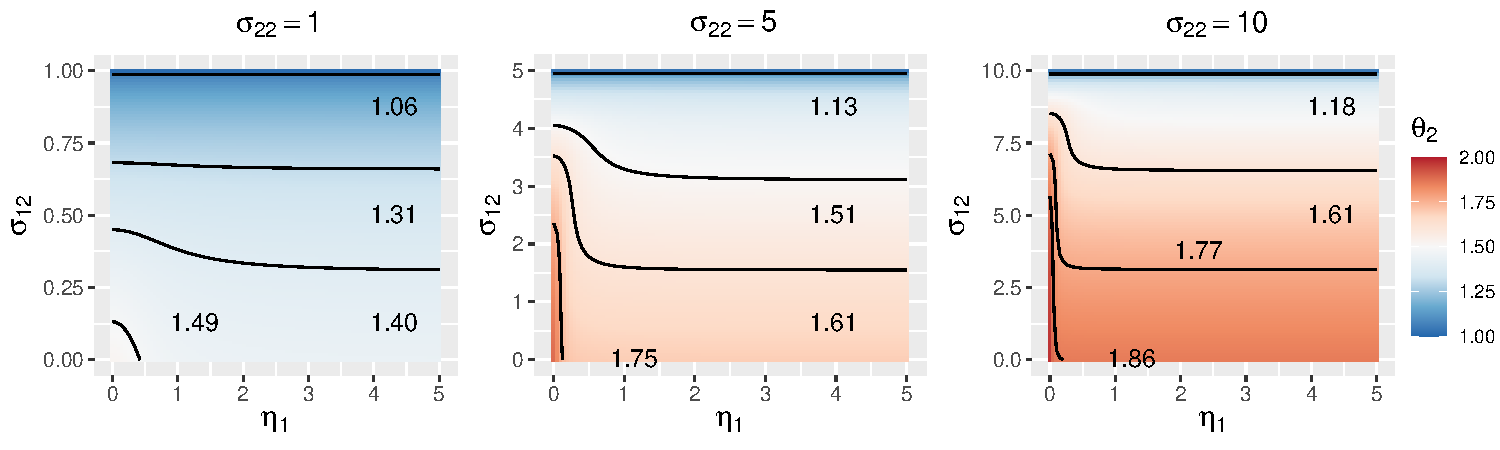
\includegraphics[width=0.95\linewidth]{bivariate_extcoef_rho_alpha.pdf}     
        \caption{}
        \label{fig:skewed_BR_extcoef}
    \end{subfigure}
    \begin{subfigure}{1\textwidth}
        \centering
        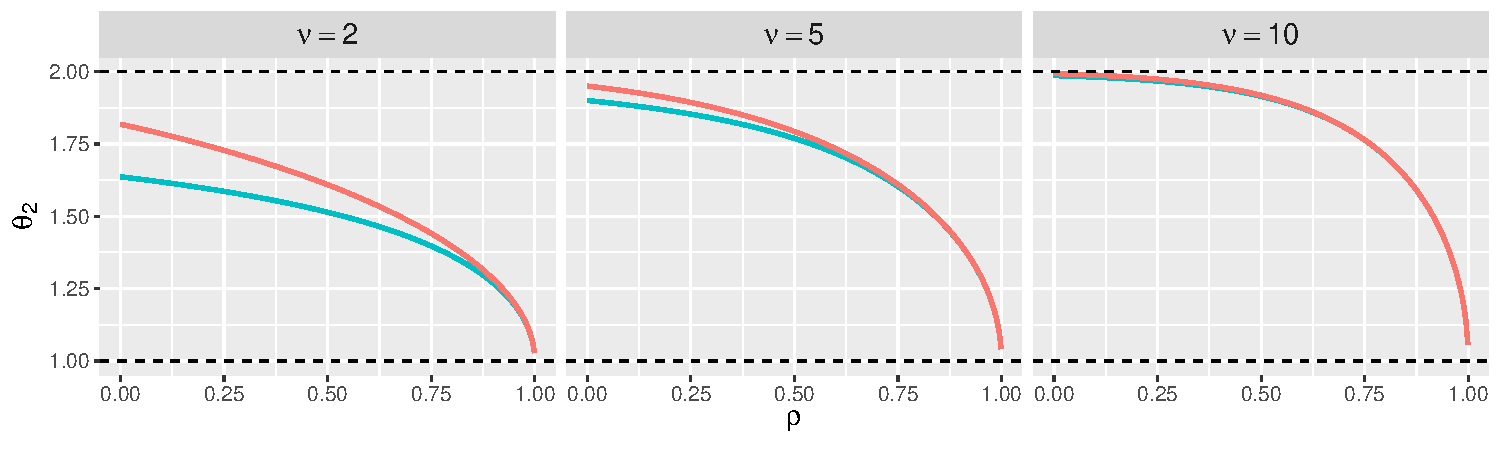
\includegraphics[width=0.95\linewidth]{bivariate_extcoef_truncT.pdf}    
        \caption{}
        \label{fig:truncated_extcoef}
    \end{subfigure}
    \caption{(a): Image plots of the bivariate extremal coefficient of the skewed Brown-Resnick model with parameters $\bm\eta = (\eta_1,-\eta_1)^\top$ and $\Sigma = ((\sigma_{22},\sigma_{12})^\top,(\sigma_{12},\sigma_{22})^\top)$ where $\sigma_{22} = 1,5$ and $10$ (left to right), as function of $\eta_1$ and $\sigma_{12}$. (b): Bivariate extremal coefficient of the truncated extremal-t process (blue) and the extremal-t process (red) with degrees of freedom $\nu=2,5$ and $10$ (left to right), as a function of the correlation parameter $\rho$.}
\end{figure}

From \eqref{eq:bi_extcoef_skewed_BR}, the bivariate extremal coefficient of the skew Brown-Resnick model depends on $\Sigma$ partly through $\gamma_{12}$, which corresponds to the semivariogram of the random vector $\bm Y$ defined in Theorem~\ref{thm:skewBR}. Whereas in the Brown-Resnick case, the extremal coefficient is fully characterised by the semivariogram.
%
Opting for a parametrisation based on semivariogram functions over covariance functions leads to greater interpretability of the model parameters and allows for asymptotic independence in the long range when considering an unbounded variogram. Indeed, taking the power-law semivariogram $\gamma(h) = (h/\lambda)^\vartheta$ for spatial lag $h$, where $\lambda>0$ and  $\vartheta \in (0,2]$ are respectively the range and smoothness parameters,
%while $h$ is the spatial lag, 
then as $h \rightarrow \infty$ we have $\bm \eta \equiv \bm \eta (h) \rightarrow \bm 0$ and therefore $\bm \xi = \bm \xi(h) \rightarrow \bm 0$ which implies that, in \eqref{eq:bi_extcoef_skewed_BR}, $\theta_2 \rightarrow 2$.
%

% However, as we see from \eqref{eq:bi_extcoef_skewed_BR}, the parameter $\Sigma$ is linked to the extremal coefficients via $\gamma_{12} = E[(W_1-W_2)^2]/2$, which is actually a semivariogram. 
% Therefore, using semivariogram functions is more interpretable than using covariance functions when fitting the (skewed) Brown-Resnick model as well as more flexible in the sense that it can bring asymptotic independence in the long range with unbounded variogram, e.g., the powered law semivariogram $\gamma(h) = (h/\lambda)^\nu$, where $\lambda$ is the range parameter, $\nu$ is the smoothness parameter, and $h$ is the distance. The construction of a stationary Brown-Resnick process using a nonstationary log-Gaussian process with an unbounded semivariogram was first introduced by \cite{Wadsworth.Tawn:2014}. 
Individually estimating the $D$ components of the parameter vector $\bm \eta$ under the constraint $\bm \eta^\top \bm 1=0$ is a difficult task. We therefore propose to represent $\bm \eta$ through spline functions. Consider the location $\bm s_i = (s_{i,1}, s_{i,2}) \in \mathcal{S}=\mathbb{R}^2$, $i=1, \ldots, D$. Let $\eta_i = \sum_{j=1}^J b_{j}K_j(\bm s_i)$, where $K_j(\bm s_i)$ is the $j$-th basis function evaluated at the location $\bm s_i$, and $b_j$ is the coefficient for the $j$th basis. The sum-to-zero constraint can be imposed by setting $\sum_{i=1}^D K_j(\bm s_i)=0$. As such, instead of trying to estimate every individual $\eta_i,i=1,\dots,D$ under the sum-to-zero condition, the coefficients $b_j,j=1,\dots,J$ for the basis functions are estimated, automatically satisfying the condition.
%
% As for the parameter $\eta$,  which is a vector with dimension $D$ and has a sum of zero. It is not very practical to estimate every component of $\eta$ individually and make it satisfy the sum-to-zero condition. Here, we use spline functions to represent the parameter $\eta$. We can write $\eta_i = \sum_{j=1}^J b_{j}B_j(\bm s_i)$, where $\bm s_i = (s_{1,i},s_{2,i})$ and $B_j(\bm s_i)$ is the $j$th basis function evaluated at the location $\bm s_i$, and $b_j$ is the coefficient for the $j$th basis. The sum-to-zero constraint can be imposed by setting $\sum_{i=1}^D B_j(\bm s_i)=0$. Therefore, instead of trying to estimate every individual $\eta_i,i=1,\dots,D$, and make sure that the sum-to-zero condition is satisfied, we can estimate the coefficients $b_j,j=1,\dots,J$ for the basis functions and the sum-to-zero condition will be automatically satisfied. 
In the remainder of this paper, $K_j(\cdot)$ denote Gaussian kernels centered at locations $\bm s_j^\star, j=1,\dots,J$, i.e.,
\begin{equation}
\label{eq:Gaussian_splines}
    K_j^\star(\bm s_i) = \phi\left(\frac{\|\bm s_i-\bm s_j^\star\|}{2\sigma_B}\right)-\frac{1}{D}\sum_{k=1}^{D}\phi\left(\frac{\|\bm s_k-\bm s_j^\star\|}{2\sigma_B}\right),\quad \text{and}\quad K_j(\bm s_i) = \frac{K_j^\star(\bm s_i)}{\sqrt{\sum_{k=1}^D K_j^\star(\bm s_k)^2}}.    
\end{equation}
%
Figure~\ref{fig:skewed_BR_extcoef_spatial} displays the bivariate extremal coefficient of the skewed Brown-Resnick model over a $[0,32]\times[0,32]$ grid, with respect to reference points labeled by a star with $J=2$, $\sigma_B = 64$ and $\eta_i = \sum_{j=1}^2 b_{j}K_j(\bm s_i) + 0.1\text{sgn}(s_{2,i}\geq 16)$, where $\bm s_1^\star=(8,8)$, $\bm s_2^\star=(24,24)$, and $\text{sgn}(\cdot)$ denotes the sign function. Note that the last term in $ \eta_i$ serves as background noise to ensure the parameter $\bm\xi = \frac{\Sigma\bm\eta}{\sqrt{1+\bm\eta^\top\Sigma\bm\eta}}$ is numerically identifiable. This is because 
%when 
multiplying $\bm\eta$ by a positive constant $c$, 
%$\bm\xi=\frac{\Sigma\bm\eta}{\sqrt{1/c^2+\bm\eta^\top\Sigma\bm\eta}}$ 
will not have numerically significant change on $\bm\xi$ as the $\bm\eta^\top\Sigma\bm\eta$ term will dominate the denominator, especially the nonstationarity introduced by the parameter $\bm\eta$ is not significant presented in the data.  
\begin{figure}[!ht]
    \centering
    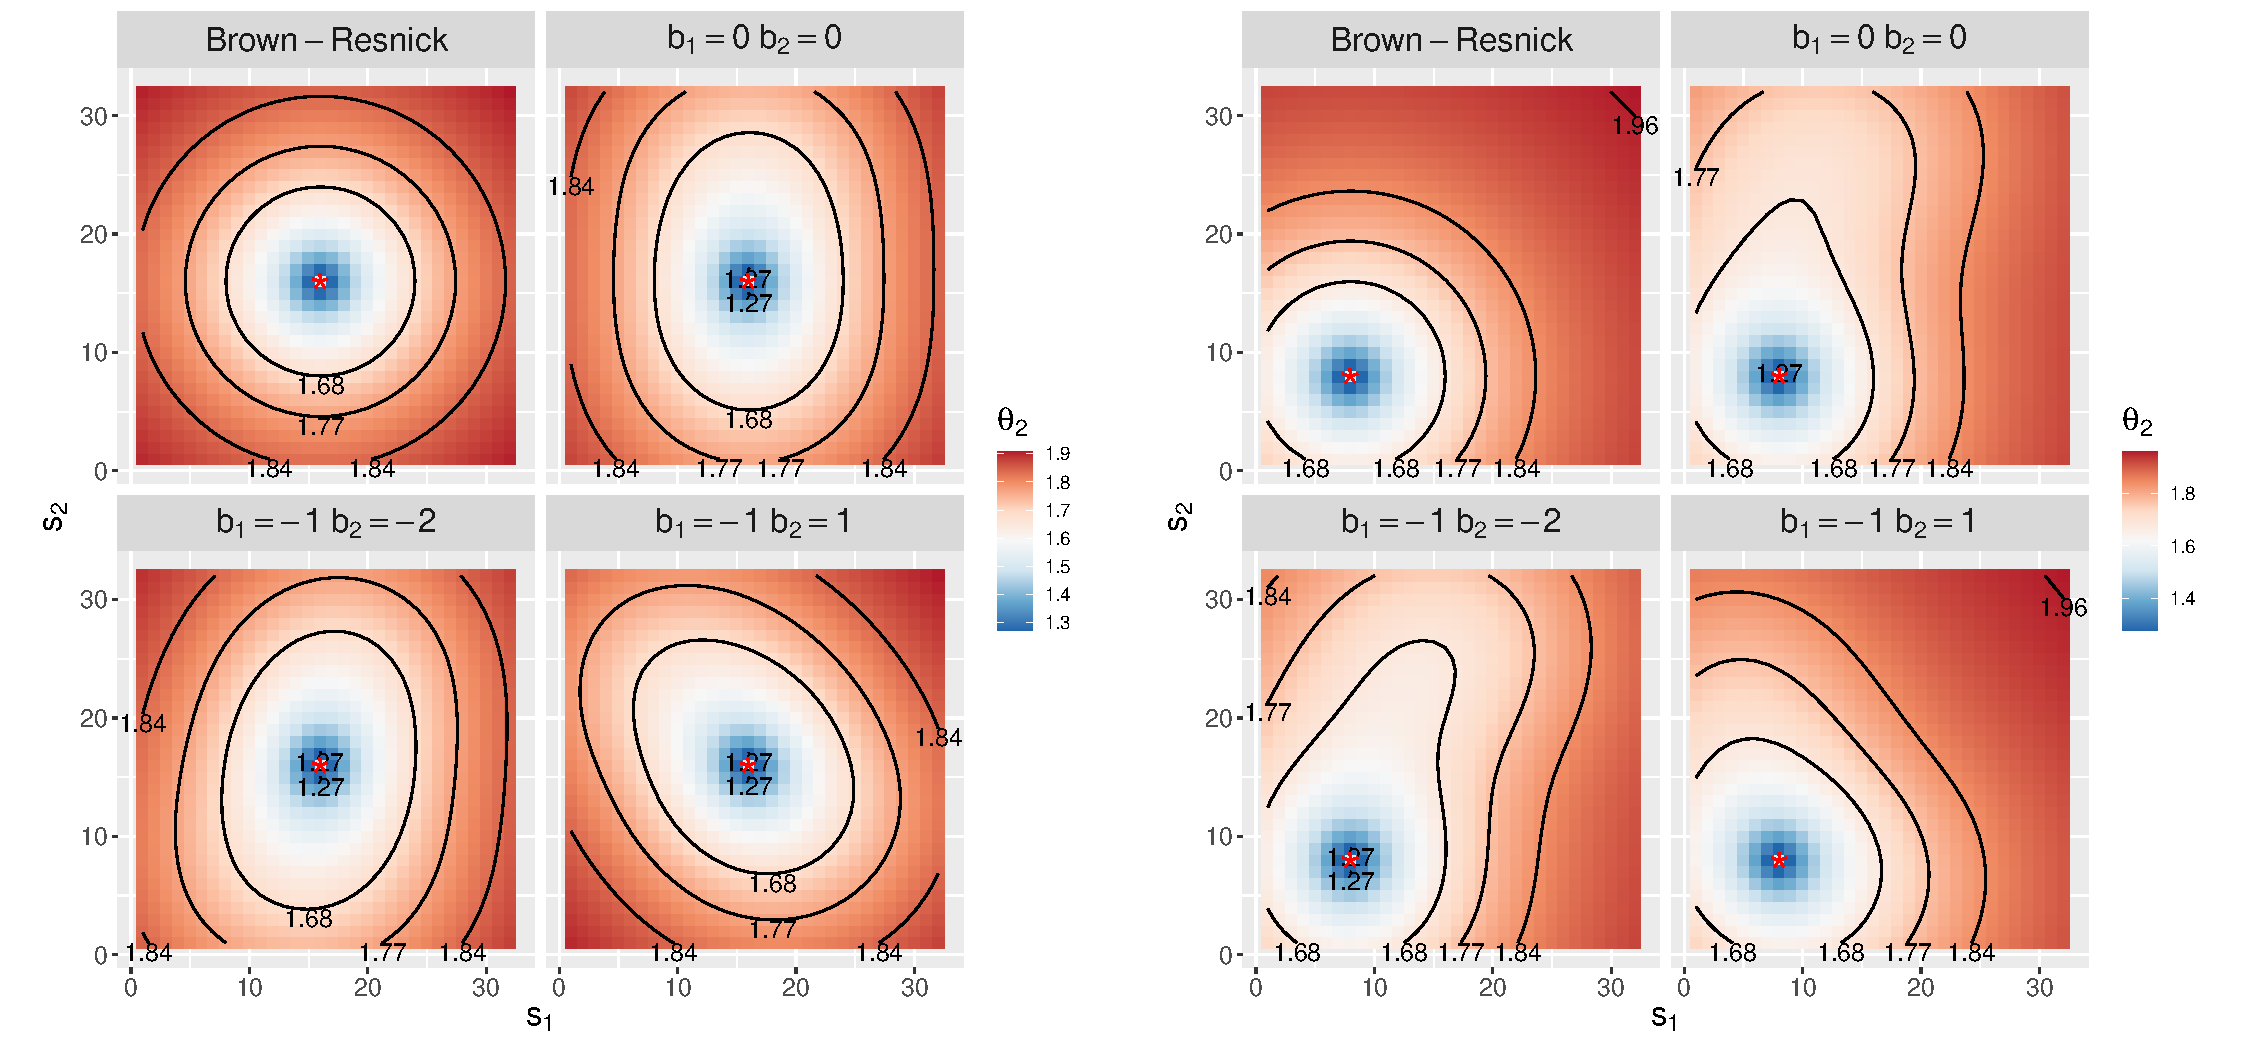
\includegraphics[width=1\textwidth]{extcoef_final_logskew.pdf}    
    \caption{Heatmaps and contour levels (solid black lines) of the bivariate extremal coefficient for the Brown-Resnick model ($\eta_i=0,i=1,\dots,D$) and skewed Brown-Resnick model where $\eta_i = \sum_{j=1}^2 b_{j}K_j(\bm s_i) + 0.1\text{sgn}(s_{2,i}\geq 16),i=1,\dots,D$ using $(b_1, b_2) = (0,0)$, $(-1,-2)$ and $(-1,-1)$. A star indicates a different basis function reference point between left and right panels.}
    \label{fig:skewed_BR_extcoef_spatial}
\end{figure}
Focusing on a single reference point (star), i.e.~on either the four left or right panels of Figure~\ref{fig:skewed_BR_extcoef_spatial}, we observe that varying the $\bm \eta$ vector through $(b_1, b_2)$ produces a broad range of dependence structures. Similarly, for fixed parameter values $(b_1,b_2)$, different dependence behaviours are observed depending on the reference point, putting the spotlight on an important feature of the skewed Brown-Resnick process: the ability to model non-stationarity and local anisotropy. This important property, exhibited by numerous real-world environmental extreme phenomena, is due to the fact that \eqref{eq:bi_extcoef_skewed_BR} not only depends on the spatial lag between two locations, but also on the corresponding components of the $\bm \xi$ parameter vector. A similar observation was made by \citet{Beranger.etal:2017} about the extremal skew-t model.

%%%%%%%%%%%%%%%%%%%%%%%%%%%%%%%%%%
\section{Inference method} %%%%%%%
\label{sec:inference} %%%%%%%%%%%%
%%%%%%%%%%%%%%%%%%%%%%%%%%%%%%%%%%

From hereon we focus on the skewed Brown-Resnick model defined through \eqref{eq:V_skBR} with the power-law semi-variogram $\gamma(h) = (h/\lambda)^\vartheta$, $\lambda>0, \vartheta \in (0,2]$ and a spline representation of $\bm \eta$, and the truncated extremal-t defined through \eqref{eq:V_tet} with the power-exponential correlation function $\rho(h) = \exp(-(h/\lambda)^\vartheta)$, $\lambda>0$, $0 < \vartheta \leq 2$. 
Traditional likelihood-based inference methods for max-stable processes have only been feasible using composite likelihoods \citep{Padoan.etal:2010,Castruccio.etal:2016}, with $k$-th order log-likelihood function defined as
\begin{equation}
\label{eq:composite}
\ell_{C;k}(\bm \theta;\bm x_1,\dots,\bm x_n)=\sum_{S \in K_k; \forall K_k} \zeta_S \sum_{i=1}^n\log g(\bm x_{i,S};\bm \theta), \quad k< D,
\end{equation}
where the first summation is over all the subsets of $\{1,\ldots,D\}$ with cardinality $k$, $g(;\bm \theta)$ is the density associated with the $k$-dimensional distribution function $G(\cdot; \bm \theta)$ as defined in \eqref{eq:ppp}, $\bm x_{i,S}$ denotes the subvector obtained by restricting $\bm x_i$ to the components indexed by $S$, and $\zeta_S \geq 0$ are some weights. Due to the form of \eqref{eq:ppp}, the joint density function is expressed as,
\begin{equation*}
\label{eq:densitymaxstable}
    g(\bm x;\bm{\theta})=\exp\{-V(\bm x;\bm\theta)\}\sum_{\pi\in \mathcal P_D}\prod_{\tau\in \pi}\left\{-V_\tau(\bm x;\bm \theta)\right\},
\end{equation*} 
where $\mathcal P_D$ is the collection of all partitions $\pi=\{\tau_1,\ldots,\tau_{|\pi|}\}$ of the set $B_D$ (of cardinality $|\pi|$) and we recall that $V_\tau$ indicates the partial derivative of the function $V$ with respect to the variables indexed by the set $\tau$. The cardinality of $\mathcal P_D$ corresponds to the $D$-th Bell number, implying that the composite likelihood function is intractable even for moderate dimensions, making inference extremely challenging. Feasible attempts have mostly focused on pairs or triples \citep{Padoan.etal:2010, Huser.Davison:2013a} while \citet{Castruccio.etal:2016} considered higher orders up to $k=11$. \citet{Stephenson.Tawn:2005} offer an alternative solution relying on observations of the partition $\pi$, referred to as hitting scenarios \citep[see also][]{Wadsworth.Tawn:2014}. \citet{Beranger.etal:2021} combined both composite and Stephenson-Tawn likelihoods to propose fast and efficient inference for the extremal skew-t process. However, the Stephenson-Tawn likelihood does not scale well with the increasing dimension, since the hitting scenarios can often involves the case that a single extreme event contributes to the maxima at a large number of locations, e.g., more than 20 when $D=225$, and thus making the Stephenson-Tawn likelihood infeasible. Most of the methods described above consider $\zeta_S=1$ when the components in $S$ are within a disk of fixed radius and $\zeta_S=0$, otherwise. This cut-off distance removes terms in \eqref{eq:composite} whose components are far away from each other but the selection of this tuning parameter is not straightforward. 

As mentioned in Section~\ref{sec:intro}, the proposed methodology for inference of max-stable models is through \eqref{eq:angular_likelihood_1} which is based on the approach in \cite{Coles.Tawn:1994} and only requires knowledge of the angular density function $h(\bm w)$. For models that only put mass on the interior of the simplex, this approach has immense potential for scalability to high dimensions since it only requires the evaluation of the angular density on $\Omega^\circ$ and avoids any other sub-spaces of $\Omega$. Theorem~\ref{thm:augular_density} establishes the conditions for a model to be fully defined by its density on $\Omega^\circ$ and Proposition \ref{prop:AngDesn_eT} \& \ref{prop:AngDesn_skBR} give a closed form expression for two new models. 
% As our models do not put mass on $\partial\Omega$, we only need to compute the angular density in the interior, $\Omega^\circ$. 
Given $n$ observations at $D$ spatial locations, $\bm x_1,\dots,\bm x_n$, and a threshold $r_0>0$, the spectral log-likelihood from \eqref{eq:angular_likelihood_1} becomes
%
\begin{equation}
\label{eq:angular_likelihood_2}
\ell_A(\bm \theta;\bm x_1,\dots,\bm x_n) = 
\sum_{i \in \{m: \|\bm x_m\| > T\}} 
\log\kappa\left(\bm x_i;\bm \theta\right). 
\end{equation} 
%
Unlike the composite likelihood estimates which are proven to be asymptotically unbiased and normally distributed, the estimates maximising \eqref{eq:angular_likelihood_2} are biased since the likelihood function is not the likelihood of the max-stable process itself but of a limiting Poisson process. The simulation experiments in the next section demonstrate that the bias can be controlled to an acceptable level by selecting an appropriate threshold $T$ and is dominated by the computational gains of the methodology. The angular density of the Brown-Resnick process is an extended skewed log Gaussian density function, which can be computed easily. For the truncated extremal-t processes, the angular density function is the truncated multivariate Student-t density after normalisation by $\bm a$. The main bottleneck is the evaluation of $\bm a$, which involves computation of the multivariate Student-t cdf, but the use of the R package \texttt{TruncatedNormal} \citep{Botev.Belzile:2021} can alleviate these issues (for dimensions up to 1000). 

As for r-Pareto processes, the likelihood-based inference can be made more straightforward by seeing the fact that the density function is proportional to the intensity function of its max-stable counterpart up to a normalising constant $\upkappa_D(\calA_r)$. The normalising constant $\upkappa_D(\calA_r)$ is generally intractable, which involves calculating a high dimensional integral in $\mathbb R_+^D$, but with $r=r_0$, we have $\upkappa_D(\calA_{r_0})=1$ and the likelihood function will be exactly the same as in \eqref{eq:angular_likelihood_2}. In other cases when $r$ is not $L_1$ norm, efforts have been made using score matching technique to avoid computing the normalising constant \citep{deFondeville.Davison:2018}. However, as suggested by Theorem~\ref{thm:r_pareto_simulation} and \citet[Proposition 2]{Dombry.etal:2024}, one can generate samples for r-Pareto processes with risk functional, $r_2$, from r-Pareto samples associated with $r_1$ risk functional using rejection sampling as long as $r_2$ is upper bounded by $r_1$ with a constant $M>0$. This allows us to use the likelihood of the r-Pareto process with the $L_1$ norm risk functional to infer the r-Pareto process with any other risk functional by choosing a high threshold $u>M$ in \eqref{eq:angular_likelihood_2}, especially for $L_p$ norm, $p\geq 1$, as all $L_p$ norms are bounded by each other. Indeed, thanks to the H\"older's inequality for $L_p$ norms, we have $r_0(\cdot)=\|\cdot\|_1 \leq D^{1-1/p}\|\cdot\|_p,\ p>1$. Therefore, we can choose $u>D^{1-1/p}, p>1$ to infer the r-Pareto process with the $L_p$ norm risk functional with the spectral likelihood in \eqref{eq:angular_likelihood_2} and produce unbiased estimators.   

Inference can be also adapted to the case when models are misspecified and the data only falls into the max-domain attraction of the model by using censored version of the likelihood-based inference method \citep{Wadsworth.Tawn:2014, Huser.etal:2016} to mitigate the bias introduced by model misspecification. However, the censored likelihood-based inference method does not scale well with increasing dimension due to the potential large number of multivariate integral involved and it is only limited to $D\leq 30$. When the censored likelihood is out of reach, but the model misspecification is a significant concern, results in \citet{Huser.etal:2016} suggest that methods using block maxima should be prefered over other methods, since taking block maxima will artificially increase the tail dependence strength between locations and push the data further towards the fitted dependence model. In the following simulation study, we will only compare the performances of composite likelihood and the spectral likelihood for max-stable processes, and for their r-Pareto counterparts, we compare the performances of the spectral likelihood and the score matching method. 

%%%%%%%%%%%%%%%%%%%%%%%%%%%%%%%%%%%%
\section{Simulation Study} %%%%%%%%%
\label{sec:sim} %%%%%%%%%%%%%%%%%%%%
%%%%%%%%%%%%%%%%%%%%%%%%%%%%%%%%%%%%

We first establish exact simulation algorithms to generate from skewed Brown-Resnick and truncated extremal-t processes, based on extremal functions \citep{Dombry.Engelke.Oesting:2016}, which are detailed in Sections~A.4 and B.4 of the Supplemental Material. \citep{Huser.etal:2016} showed that the spectral likelihood method is more efficient than the composite likelihood method for the logistic model, whose distribution does not put mass on the boundary space, when the extremal dependence is relatively strong, but its performance is still comparable with the composite likelihood when the extremal dependence is weak especially with relatively large sample sizes ($D=30$ and $n=10^4$ in their case). Here, we conduct comparison between the spectral likelihood and the composite likelihood for the Brown-Resnick model with simulated samples of size $n=500$ on a $15\times15$ grid (i.e, $D=225$). The parameters are chosen to be $\lambda=3,6$ and $\vartheta=0.5,1,1.5$ (6 combinations). The threshold $T$ used in the spectral likelihood is taken to be $T=30\times D$, resulting in retaining around 16 observations, and the cut off distance for the pairwise likelihood is set to be $2\sqrt{2}$ yielding 2268 pairs for likelihood calculation. Figure~\ref{fig:simulation_boxplot_BR} displays violin plots of the 300 replicate estimated parameters $\hat\lambda$ and $\hat\vartheta$ from the Brown-Resnick model using spectral (red) and composite likelihoods (blue), where true parameter values are indicated by dots. Results shows that when the dependence strength is relatively weak (i.e., small $\lambda$ and large $\vartheta$), the spectral likelihood method tends to be more biased, and it overestimates the range parameter $\lambda$ but underestimate the smoothness parameter $\vartheta$. However, in that case, the spectral likelihood estimator will be less viable since data with week dependence possess more effective independent samples. The pairwise likelihood estimator produce unbiased estimates and is also less viable than the spectral likelihood estimator due to the large number of observations used. As for speed of the computation, the spectral likelihood method only take 9.2 seconds on average with 3 CPU cores. In contrast, the pairwise likelihood takes an average of 13.7 minutes with 16 CPU cores, which is about 476 times slower in terms of core hours than the spectral likelihood. As dimension ($D$) increases, we can expect the relative performance of the spectral likelihood to the composite likelihood to improve due to more available data (higher $T$, so less bias) and more terms in the composite likelihood.     
%
\begin{figure}[!ht]
    \centering
    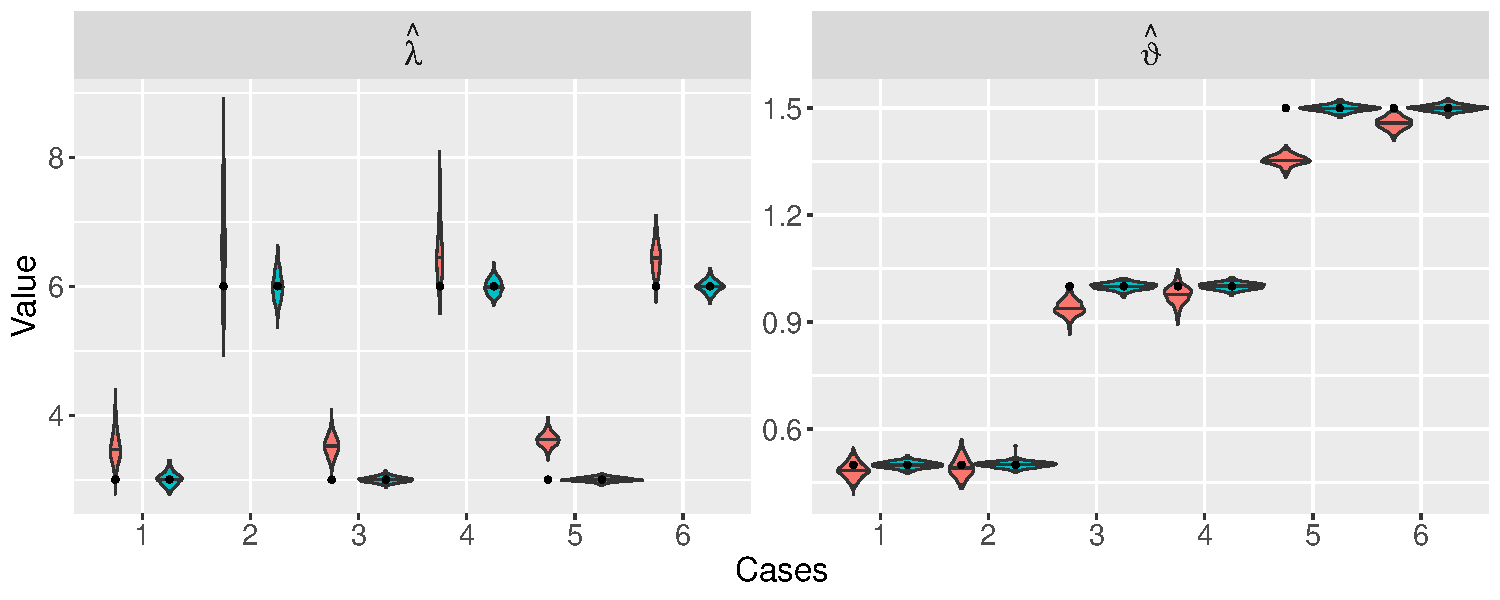
\includegraphics[width=1\textwidth]{simulation_est_boxplots_final_BR_30.pdf}    
    \caption{Violin plots for 300 replicate estimates of $\bm \theta = \left(\lambda, \vartheta\right)$ for the Brown-Resnick process with $\lambda=3,6$ and $\vartheta=0.5,1,1.5$ using the spectral likelihood (red) and the pairwise likelihood (blue) with 2268 pairs. Black dots indicate the true values.}
    \label{fig:simulation_boxplot_BR}
\end{figure}
%
The pairwise likelihood method is unbiased for Brown-Resnick processes, but it is computationally expensive. Moreover, for our new models, the pairwise likelihood method is not available for truncated extremal-t processes as the marginal 
distribution of a multivariate truncated normal is not a truncated normal. This necessitates a costly numerical integration for each composite likelihood term \citep{Horrace:2005}, and for skewed Brown-Resnick processes, we found the pairwise likeihood estimators for the skewness parameter $b_1$ and $b_2$ to be unreliable. As an illustration, we performed a small comparative study based on datasets of 500 observations with parameters $\lambda=3$, $\vartheta=1$, and $(b_1,b_2) = (-1,-2)$, generated on the same $15\times15$ grid, where the centres of the kernels are chosen to be $\bm s_1^\star = (4,4)$ and $\bm s_2^\star=(11,11)$. For the spectral likelihood, the higher the threshold $T$ the better the Poisson approximation to the true likelihood, but simultaneously the fewer observations available. As we have fewer observations (for computational tractability), we choose a threshold of $T = 30\times D$ for the spectral likelihood approach. For the pairwise likelihood, we use the 1202 closest pairs for likelihood calculation due to the computational overheads. Figure~\ref{fig:simulation_boxplot_skewedBR_comp} shows the 300 replicate estimates of $\lambda$, $\vartheta$, $b_1$, and $b_2$ for both spectral and pairwise likelihoods. The spectral likelihood provides almost unbiased estimates for the parameters $b_1$ and $b_2$ and the expected small relative bias (around $10\%$) for $\lambda$ and $\vartheta$. In contrast, the pairwise likelihood provides unbiased estimates for $\lambda$ and $\nu$, but biased and almost unreliable estimates with large variability for $b_1$ and $b_2$, which may due to the pairwise likelihood cannot capture the locally anisotropic dependence structure presented in the data. Again, the pairwise likelihood is also more computationally expensive, taking around 2.36 hours on average using a 16-core machine, compared to 124.4 seconds on average for the spectral likelihood using 16-core machine with multiple initial values for the skewness parameter to avoid local optimal. 
%
\begin{figure}[!ht]
    \centering
    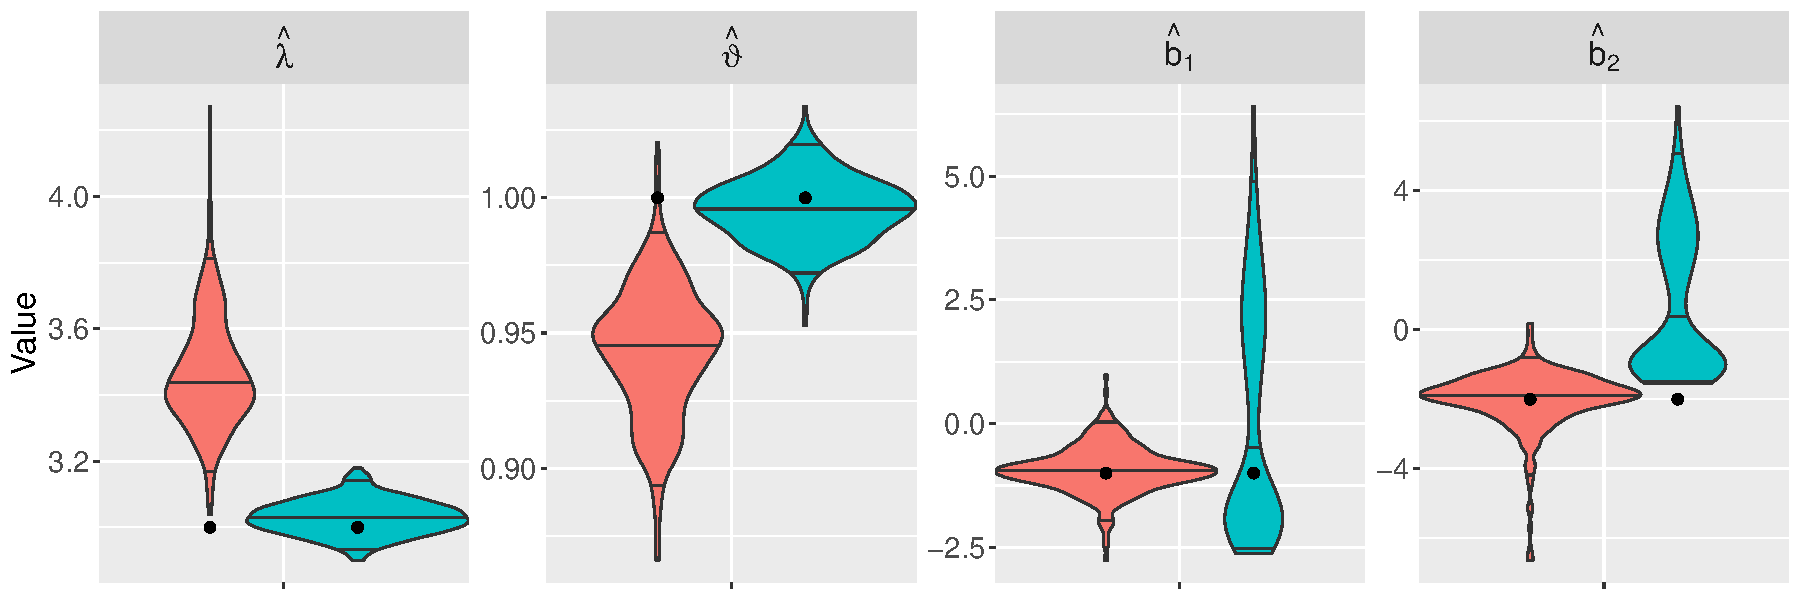
\includegraphics[width=1\textwidth]{simulation_est_boxplots_final_skewBR_comp.pdf}
    \caption{Violin plots for 300 estimates of $\bm \theta = (\lambda, \vartheta, b_1, b_2)$ for the skewed Brown-Resnick process with $\lambda=3$, $\vartheta=1$, and $(b_1,b_2) = (-1,-2)$ using the spectral likelihood (red) with threshold $T=30\times D$ and the pairwise likelihood (blue) with 1202 pairs. Black dots indicate the true values.}
    \label{fig:simulation_boxplot_skewedBR_comp}
\end{figure}
%   

To further demonstrate the spectral method with our new models, we generate 2000 observations from the skewed Brown-Resnick model with $\lambda=5,10$, $\vartheta = 1,1.5$, and $(b_1,b_2) = (0,0),(-1,-2),(-1,1)$ (12 combinations), where the centres of the kernels are chosen to be $\bm s_1^\star = (4,4)$ and $\bm s_2^\star=(11,11)$ and 2000 observations from the truncated extremal-t on a $10\times10$ grid (i.e., $D=100$) with $\lambda=1,3$, $\vartheta=1$ and $\nu=2$ (2 combinations). For skewed Brown-Resnick model, parameters are estimated by maximising the spectral likelihoods and this procedure is repeated 300 times. For the truncated extremal-t model, we investigate the impact of the threshold $T$ on the estimation performance of the spectral likelihood estimator. The threshold is set to be the $90\%, 95\%$, and $98\%$ quantiles of the observed radial components. As we have more observations, we choose $T = 100\times D$ for the skewed Brown-Resnick model resulting in about 20 observations retained. The bias in the spectral likelihood will reduce as the threshold $T$ increases (see e.g.~Figure \ref{fig:simulation_boxplot_truncT}, below), although in practice increasing thresholds will reduce the data available for model fitting. Figure~\ref{fig:simulation_boxplot_truncT} shows violin plots for the estimates of the range and smoothness parameters for the truncated extremal-t model, where the degree of freedom is fixed at its true value ($\nu=2$), and the threshold $T$ is chosen to be the $98\%$ (red), $95\%$ (green), and $90\%$ (blue) empirical quantiles of the radial component. For the sample size of $n=2000$ observations, retaining the $2\%$ of observations (i.e., 40) with the largest radial components produces almost unbiased estimates. Lowering this threshold increases the bias but also increases the computation time since more observations are included. As highlighted in Section~\ref{sec:theory}, fitting the truncated extremal-t model requires more computational effort than the skew Brown-Resnick model, here requiring a mean of about 15 minutes on a $10 \times 10$ grid ($D=100$).
%
\begin{figure}[!ht]
    \centering
    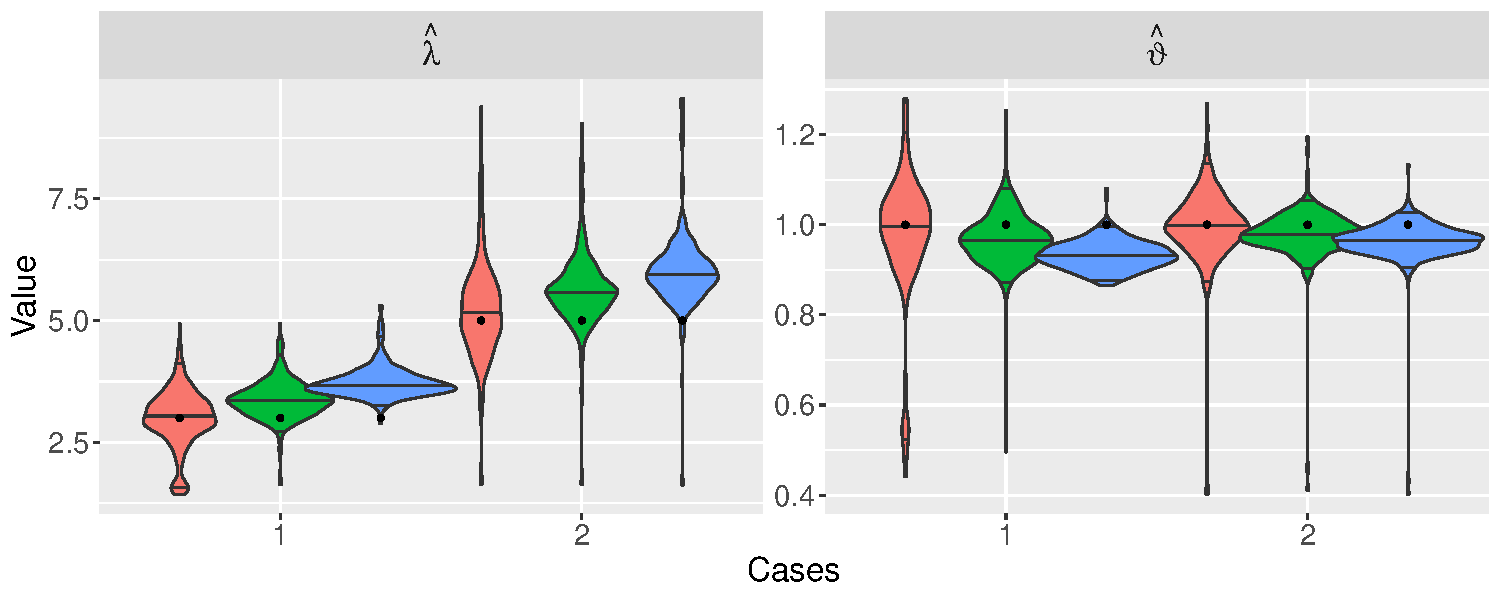
\includegraphics[width=1\textwidth]{simulation_est_boxplots_final_truncT.pdf}    
    \caption{Violin plots for 300 estimates of $\bm \theta = (\lambda, \vartheta, 2)$ for the truncated extremal-t process with $\lambda=3,6$, $\vartheta=1$, and $\nu=2$, using the spectral likelihood. The threshold $T$ is set to be the $98\%$ (red), $95\%$ (green) and $90\%$ (blue) empirical quantiles of the radial component. Black dots indicate the true values.}
    \label{fig:simulation_boxplot_truncT}
\end{figure}
%
Figure~\ref{fig:simulation_boxplot_skewedBR} shows parameter estimates for the skew Brown-Resnick process using the spectral likelihood, for the 12 parameter combinations. The estimates for $\lambda$ and $\vartheta$ are more accurate than those estimates shown in Figure~\ref{fig:simulation_boxplot_BR}, due to the larger sample size and higher threshold $T$. In particular, the estimates of the skewness-related parameters $(b_1,b_2)$ are all identifiable and almost unbiased.
Model fitting is computationally efficient, with each fit taking around $6$ minutes on average using 16 cores with multiple initial values for the skewness parameter.
\begin{figure}[!ht]
    \centering
    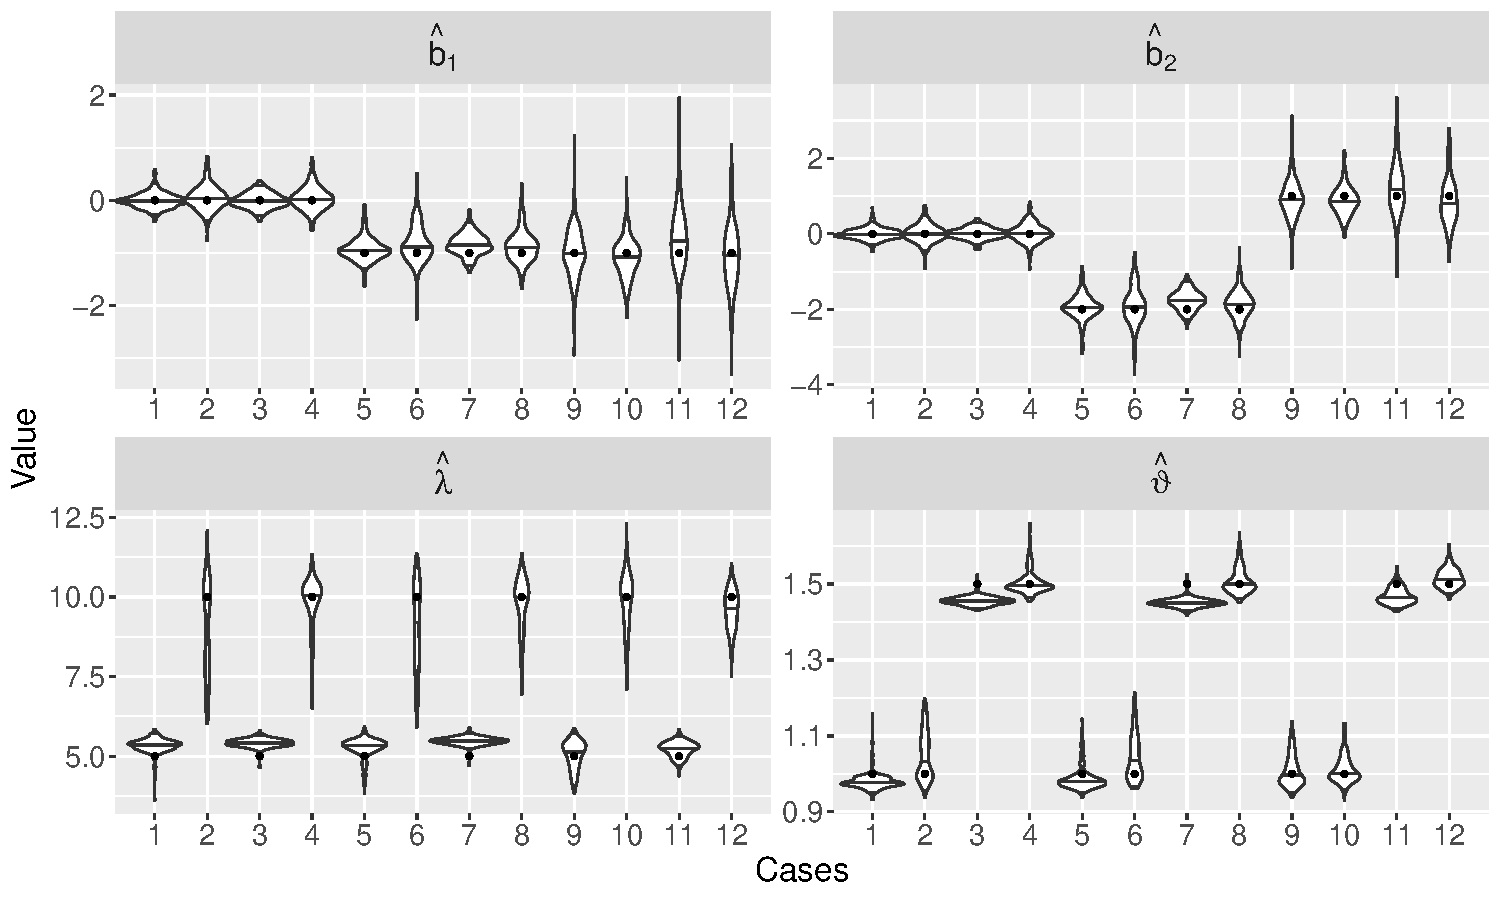
\includegraphics[width=1\textwidth]{simulation_est_boxplots_final.pdf}    
    \caption{Violin plots for the 300 estimates of $\bm \theta= \left(\lambda, \vartheta,  b_1, b_2\right)$ for the skewed Brown-Resnick process with $\lambda=5,10$, $\vartheta=1,1.5$, and $(b_1,b_2) = (0,0),(-1,-2),(-1,1)$, using the spectral likelihood. Black dots indicate the true values.}
    \label{fig:simulation_boxplot_skewedBR}
\end{figure}
%
For r-Pareto couterparts of the skewed Brown-Resnick processes, we simulate 2000 r-Pareto observations on a $15\times15$ grid with the same parameter configuration as in Figure~\ref{fig:simulation_boxplot_skewedBR} and two risk functinals $L_1$ norm and the $L_3$ norm. Then, we compare the inference using the score matching method (see more details in \citet{deFondeville.Davison:2018}) and the spectral likelihood method. In both method, the threshold $u$ are chosen to be $95\%$ empirical quantiles of $r(\bm X_1),\dots,r(\bm X_n)$. Figure~\ref{fig:simulation_boxplot_rpareto_skewedBR} shows the violin plots based on 300 fitted results with risk functional being $L_3$ norm and similar results can be also found for the $L_1$ norm case. The spectral likelihood method produces unbiased estimates for all the parameters including the skewness parameters with small variability. The score matching method produces almost unbiased estimates for the parameters $\log(\lambda)$, $\vartheta$, but is numerically unstable to reasonably estimate the skewness parameters. The median of the 300 estimates for the paramters $b_1$ and $b_2$ are close to the true values but with large variabilities. As for computational speed, the spectral liklihood method takes around 141 seconds using 3 CPU cores without the needs to use multiple initial values, while the score matching method takes around 704 seconds using the same amount of CPU cores and is 5 times slower than the spectral likelihood method.
%
\begin{figure}[ht]
    \centering
    \includegraphics[width=1\textwidth,page=2]{simulation_pareto_violin__5_Inf_Inf.pdf}    
    \caption{Violin plots for the 300 estimates of $\bm \theta= \left(\lambda, \vartheta,  b_1, b_2\right)$ for the r-Pareto process based on skewed Brown-Resnick processes with risk functional $L_3$ norm and the same parameter configurations as in Figure~\ref{fig:simulation_boxplot_skewedBR} using the spectral likelihood (right 4 panels) and score matching method (left 4 panels). Black dots indicate the true values.}
    \label{fig:simulation_boxplot_rpareto_skewedBR}
\end{figure}
%
We also generated 2000 r-Pareto observations based on the truncated extremal-t processes on a $8\times8$ grid with $\lambda=(3,5)$, $\vartheta=(1,1.5)$, and $\nu=2,3$ (8 combinations) and two risk functionals $L_1$ norm and the $L_3$ norm. The spectral likelihood method is used to estimate the parameters $\log(\lambda)$ and $\vartheta$ and the results are shown in Figure~\ref{fig:simulation_boxplot_rpareto_truncT}. The spectral likelihood method and the score matching produces almost unbiased estimates for $\hat\vartheta$. However, for the range parameter $\hat\lambda$, the spectral likelihood method produces $20\%$ relative bias, while the score matching method again shows numerical instability. The spectral likelihood method takes around 126 seconds using 3 CPU cores, while the score matching method takes around 10 times longer using the same amount of CPU cores.

\begin{figure}[!ht]
    \centering
    \includegraphics[width=1\textwidth,page=4]{simulation_pareto_violin__5_Inf_Inf.pdf}    
    \caption{Violin plots for the 300 estimates of $\bm \theta= \left(\log(\lambda), \vartheta\right)$ for the r-Pareto process based on truncated extremal-t processes with risk functional $L_3$ norm, where $\lambda=c(3,5),\vartheta=(1,1.5)$ and $\nu$ is fixed to be either 2 (case 1--4) or 3 (case 5--8), using the spectral likelihood (right 2 panels) and score matching method (left 2 panels). Black dots indicate the true values.}
    \label{fig:simulation_boxplot_rpareto_truncT}
\end{figure}
The experiments conducted in this section for max-stable processes indicate that, for an appropriately selected threshold, the spectral likelihood approach can produce almost unbiased estimates with accuracy comparable to, and better than (for the skewed Brown-Resnick) the pairwise likelihood, at the fraction of the computational cost. For r-Pareto counterparts, the spectral likelihood method shows great efficiency and great numerical stability in estimation producing unbiased estimator with small variability, compared to the score matching method. 

\section{Application}
\label{sec:application}
We now examine the spatial dependence structure of the radar measurements of rainfall data during the wet season, June--September, in Tampa Bay area, Florida. The data consist of every 15 minutes measurements taken at a regular 2km grid with 4449 locations, from 1995 to 2019. There are $n=139881$ observations in total. Part of the data has been fitted to a r-Pareto process based on Brown-Resnick model in \cite{deFondeville.Davison:2018}, where they used 3600 spatial locations from 1999 to 2004. Here, we follow the same fitting procedure as in \citet{deFondeville.Davison:2018} except we fit a skewed Brown-Resnick model to the whole dataset to demonstrate the spectral likelihood method and the flexibility of our model. The data are first transformed to the unit Pareto scale using the empirical distribution functions location by location for convenience, while the zero values in the dataset are ignored and are treated as missing. We also adopted an anisotropic semivariogram function 
\begin{equation}
    \gamma(\bm h) = \left\|\frac{\bm h^T V \bm h}{\lambda}\right\|_2^\vartheta, \vartheta\in(0,2],\lambda>0,
\end{equation}
where $\bm h$ is the difference vector between coordinates in two locations and $V$ is an anisotropy matrix used to capture the global anisotropy in the dependence structure
\begin{equation}
    V = \begin{pmatrix}
    \cos\zeta & - \sin\zeta\\
    m\sin\zeta &  m\cos\zeta
    \end{pmatrix}, m >0 , \zeta\in (-\frac{\pi}{4},\frac{\pi}{4}).
\end{equation}
To fit the r-Pareto processes, we again choose the $L_1$ norm and the $L_\infty$ norm as the risk funcational. With the $L_\infty$ norm, the model will pick up events with local intense rainfall at any location of the region, while $L_1$ norm will tends to pick up events with high cumulative rainfall over the whole region. We then fit a univariate generalized Pareto distribution to the values of risk functional evaluated at each observations and check the threshold where the estimated shape parameter become stable so that we can choose the same threshold for each of the risk functional we use. For both of the risk functional, we choose the threshold $u$ to be the $99.95\%$ empirical quantiles of $r(\bm X_1),\dots,r(\bm X_n)$, resulting in 70 observations left for the model fit. Then, We fit two nested models, the skewed Brown-Resnick r-pareto process and the Brown-Resnick r-Pareto process, which is a sub model for the skewed Brown-Resnick model when the skewness parameters are set to be zero. For the Brown-Resnick process, each fit took around 51 mintues using a 16-core machine, while it took around 8 hours to fit a skewed Brown-Resnick model since it has 4 extra parameters for the skewness parameters. Table~\ref{tab:parameter_estimates} shows the parameter estimates for the two models based. The estimated $\hat m$ shows no significant differences from 1 in all the cases. It implies that there is no global anisotropy in the dependence structure, which is consistent with the results in \cite{deFondeville.Davison:2018}. However, the estimated slant parameters $b_1$ to $b_4$ are significant from zero, which indicates local anisotropic dependence structure is detected by the skewed Brown-Resnick model. The bivariate extremal coefficients for the skewed Brown-Resnick model are shown in Figure~\ref{fig:extcoef_application}, where the extremal coefficients are higher along the north-south axis, which is consistent with the anisotropy matrix used in the model. Figure~\ref{fig:extcoef_application_florida} shows the maps of bivariate extremal coefficients with respect to two different reference points, and the fitted extremal coefficient contour curves with 8 levels, 1.2,1.5,1.7,1.75,1.8,1.85,1.9, and 1.95. The extremal coefficient contour curves for the skewed Brown-Resnick model are able to pick up the directional anisotropic pattern presented by the empirical estimates and the patterns changes with the reference location. With the $L_\infty$ norm risk functional, the estimated extremal dependence is more localised, while with the $L_1$ norm risk functional, the estimated extremal dependence is more persistent in distance, which are coherent with the interpretation of the extreme events picked by these risk functional. 
%
\begin{table}[!ht]
    \centering
    \scalebox{0.9}{
        \begin{tabular}{ccccccccc}
            \hline
           Model & $\hat\lambda$ & $\hat\vartheta$ & $\hat\zeta$ & $\hat m$ & $\hat b_1$ & $\hat b_2$ & $\hat b_3$ & $\hat b_4$ \\ 
            \hline
            1 & 600.16 & 115.62 & 78.53 & 99.06 & - & - & - & - \\ 
              & (392.57) & (10.6) & (1.94) & (13.91) & - & - & - & - \\ 
            2 & 533.4 & 137 & 19.63 & 92.76 & - & - & - & - \\ 
              & (44.56) & (3.04) & (0.46) & (5.67) & - & - & - & - \\ 
            3 & 483.66 & 119.31 & 19.63 & 103.86 & 1541.7 & 1136.9 & 3132.16 & 2658.78 \\ 
              & (132.11) & (10.51) & (0) & (4.35) & (0.03) & (0.02) & (0.01) & (0.02) \\ 
            4 & 504.38 & 140.78 & 19.63 & 93.72 & 32.29 & 25.76 & 9.03 & 14.33 \\ 
              & (28.18) & (3.08) & (0.88) & (5.21) & (0.4) & (0.37) & (0.52) & (0.43) \\ 
            \hline
        \end{tabular}
    }
    \caption{Parameter estimates with standard errors in parentheses based on jackknife estimates. Model 1 is the Brown-Resnick r-Pareto process with $L_1$ norm risk functional, Model 2 is the Brown-Resnick r-Pareto process with $L_\infty$ norm risk functional, Model 3 is the skewed Brown-Resnick r-Pareto process with $L_1$ norm risk functional, and Model 4 is the skewed Brown-Resnick r-Pareto process with $L_\infty$ norm risk functional. All numbers are multipled by $100$.}
    \label{tab:parameter_estimates}
\end{table}
%
\begin{figure}[!ht]
    \centering
    \begin{subfigure}{0.45\textwidth}
        \centering
        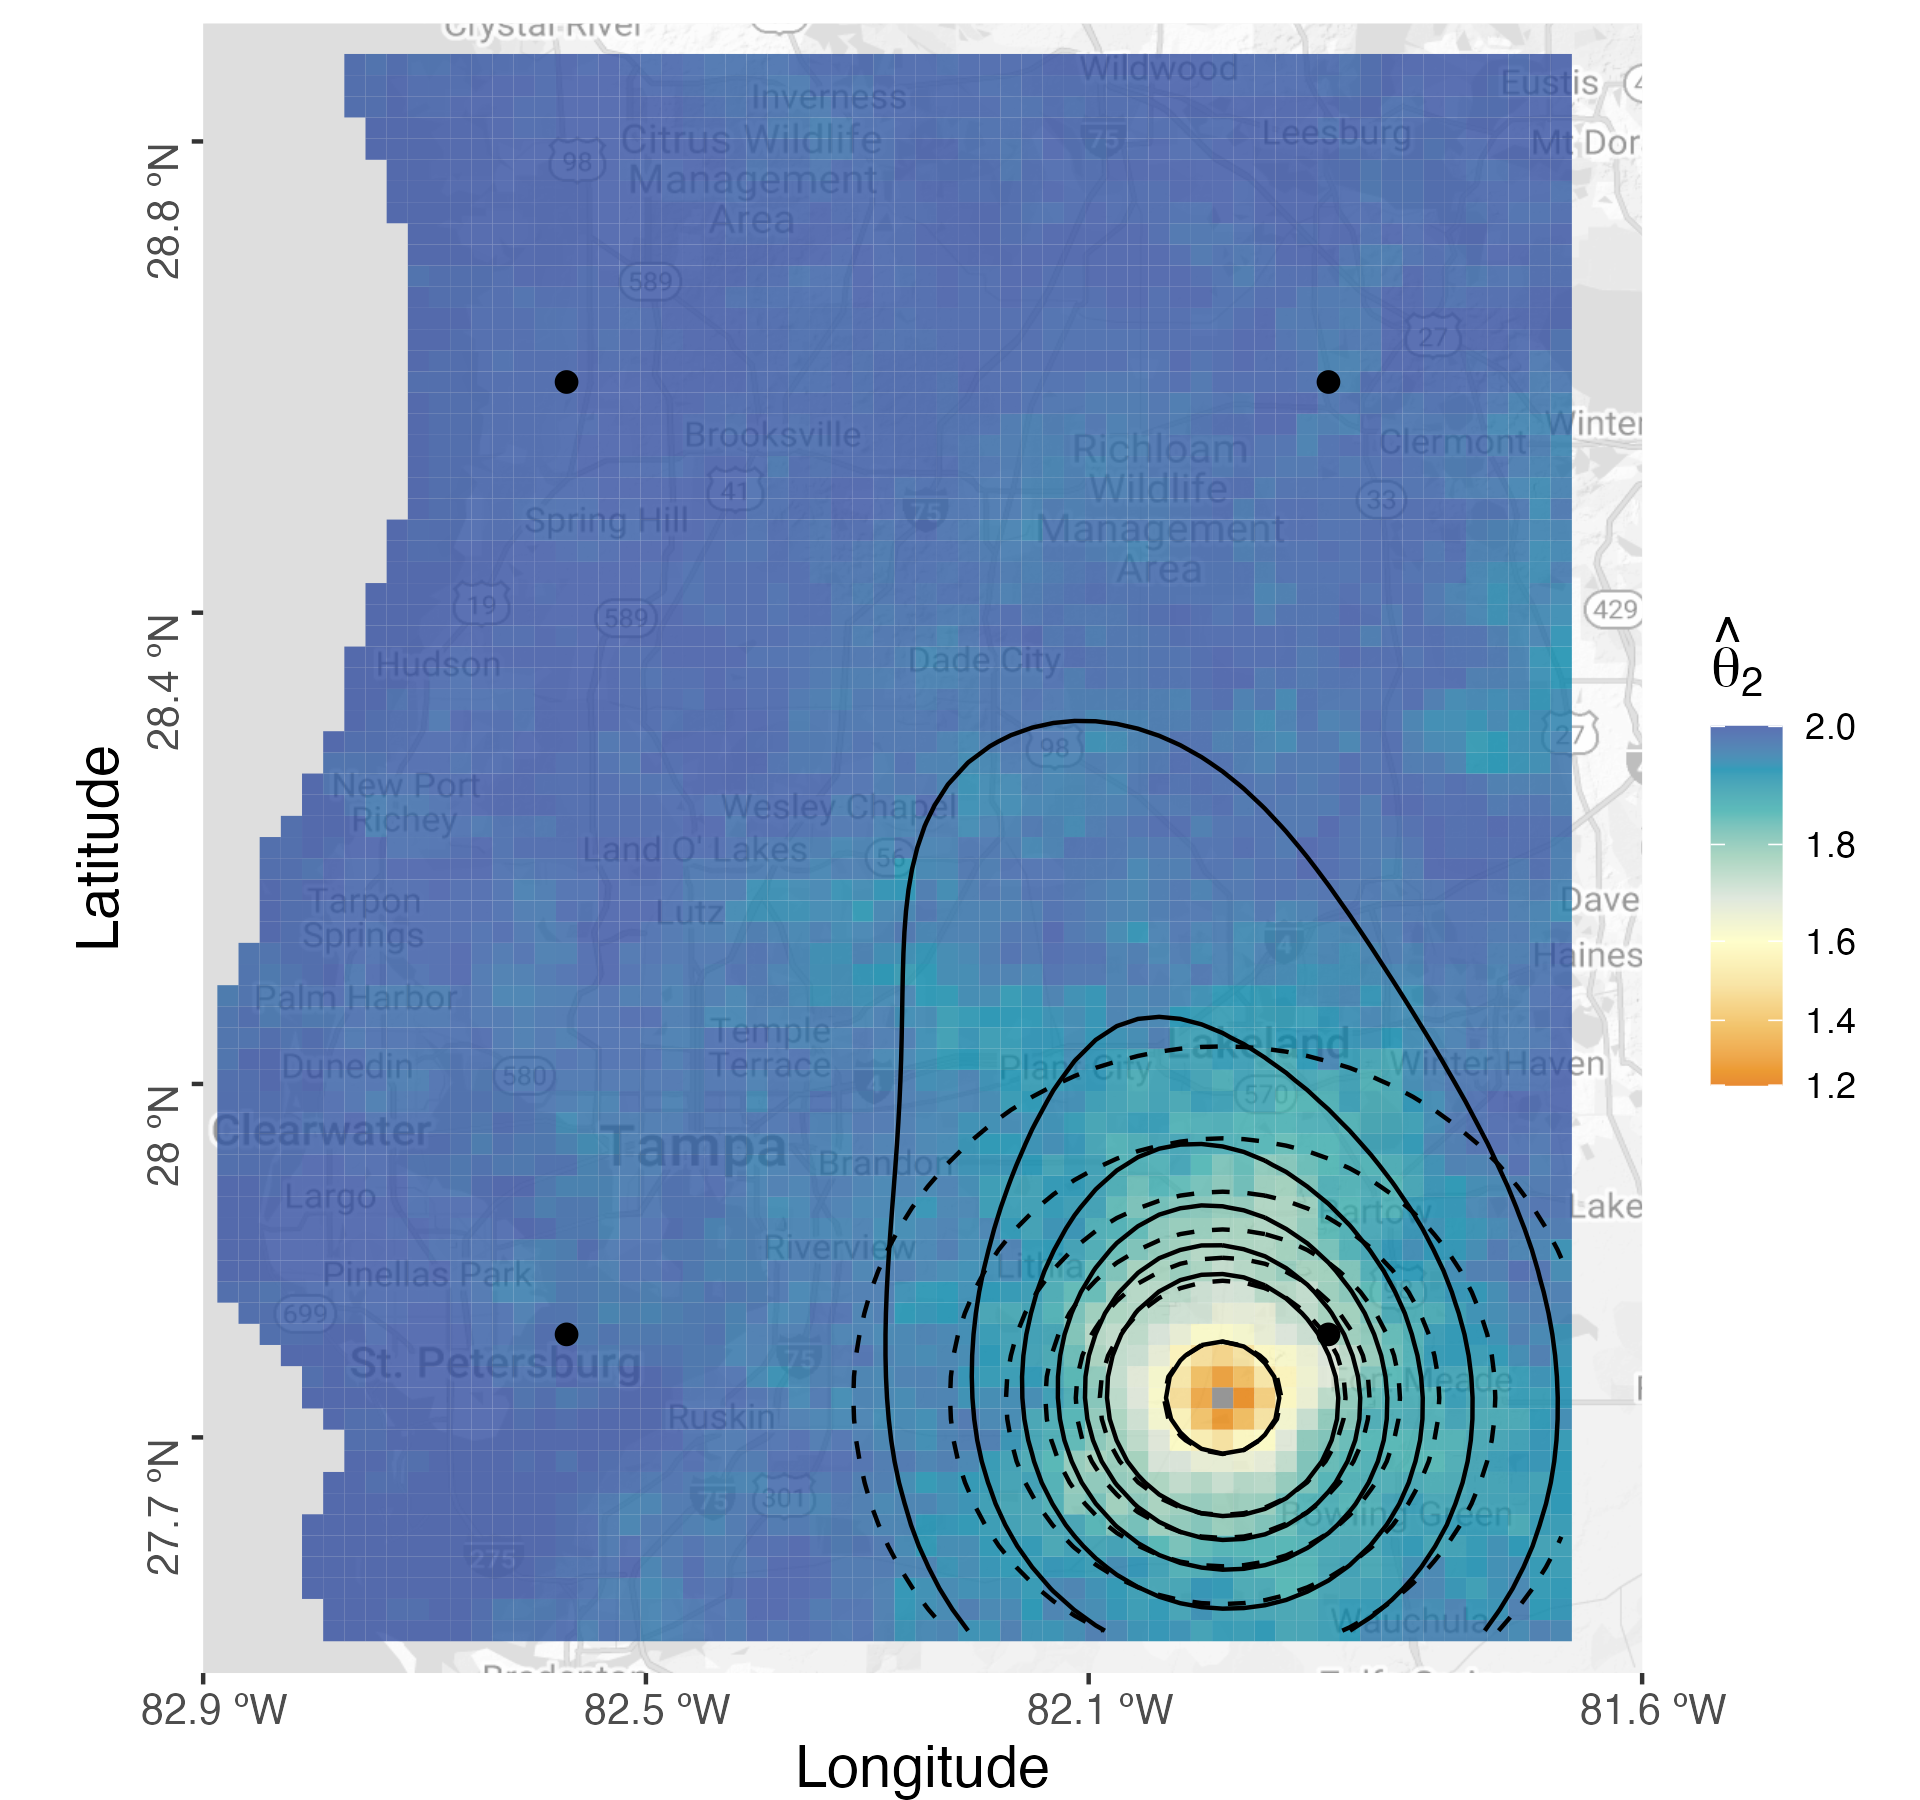
\includegraphics[width=1\textwidth]{florida/florida_extcoef_1_005.png}
    \end{subfigure}%
    \begin{subfigure}{0.45\textwidth}
        \centering
        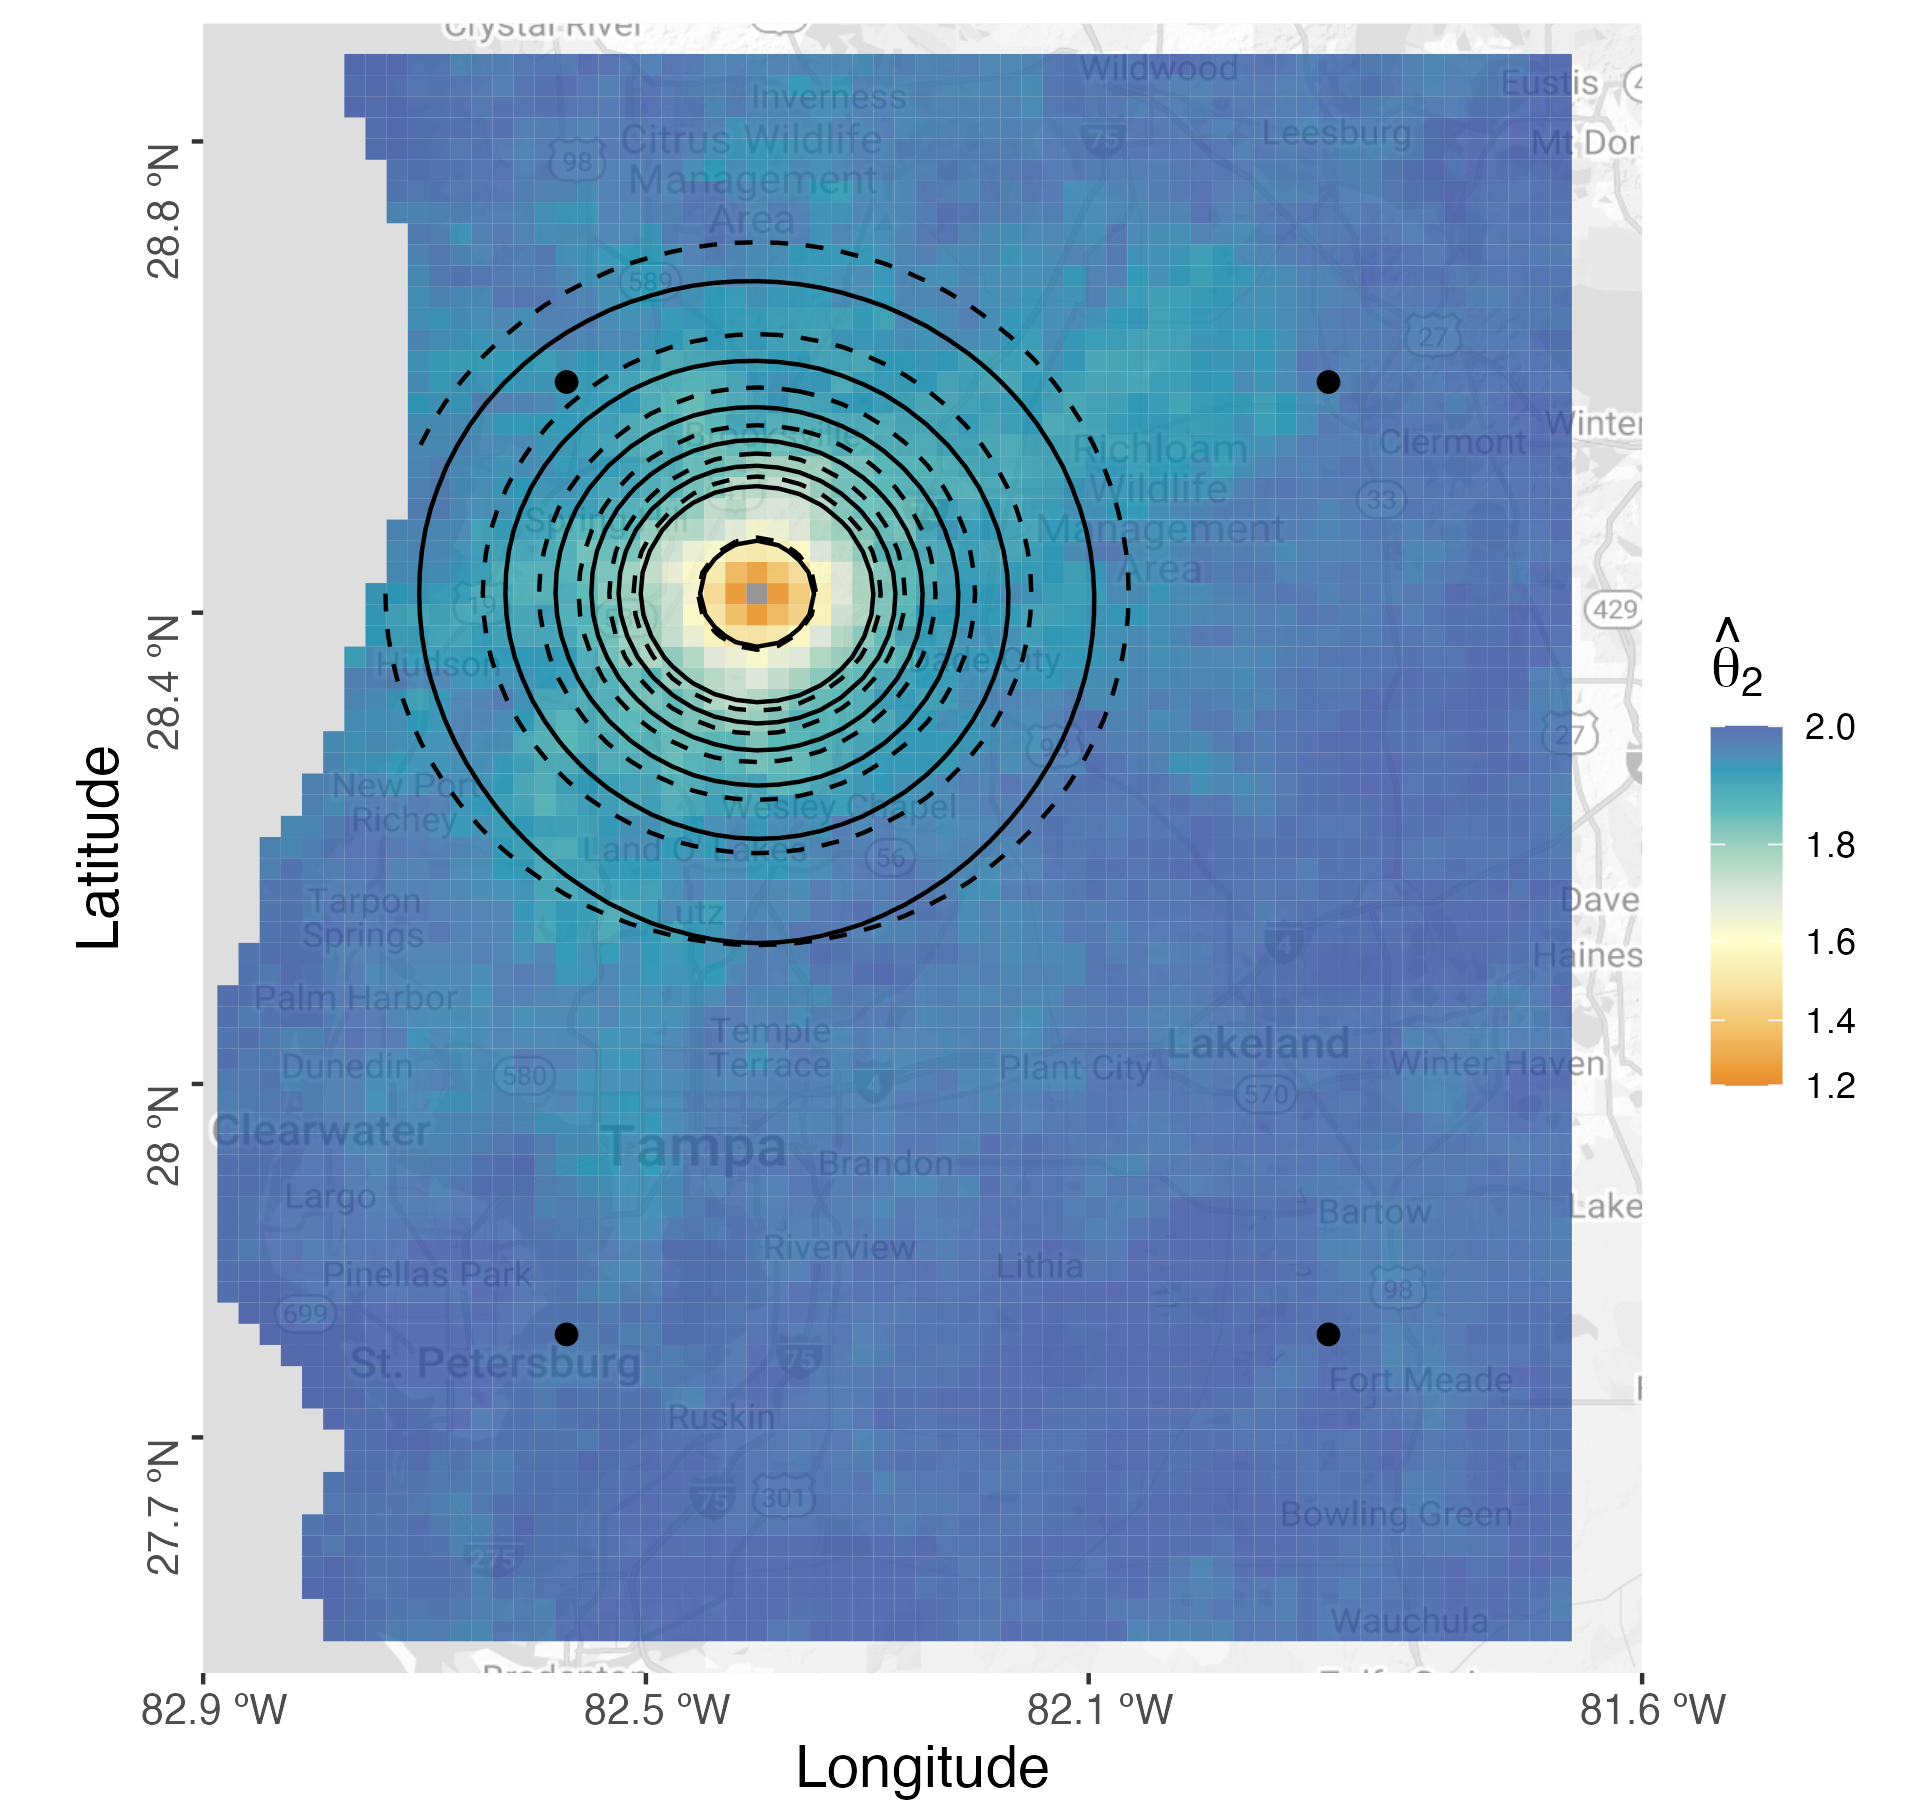
\includegraphics[width=1\textwidth]{florida/florida_extcoef_1_034.png}
    \end{subfigure}
    \begin{subfigure}{0.45\textwidth}
        \centering
        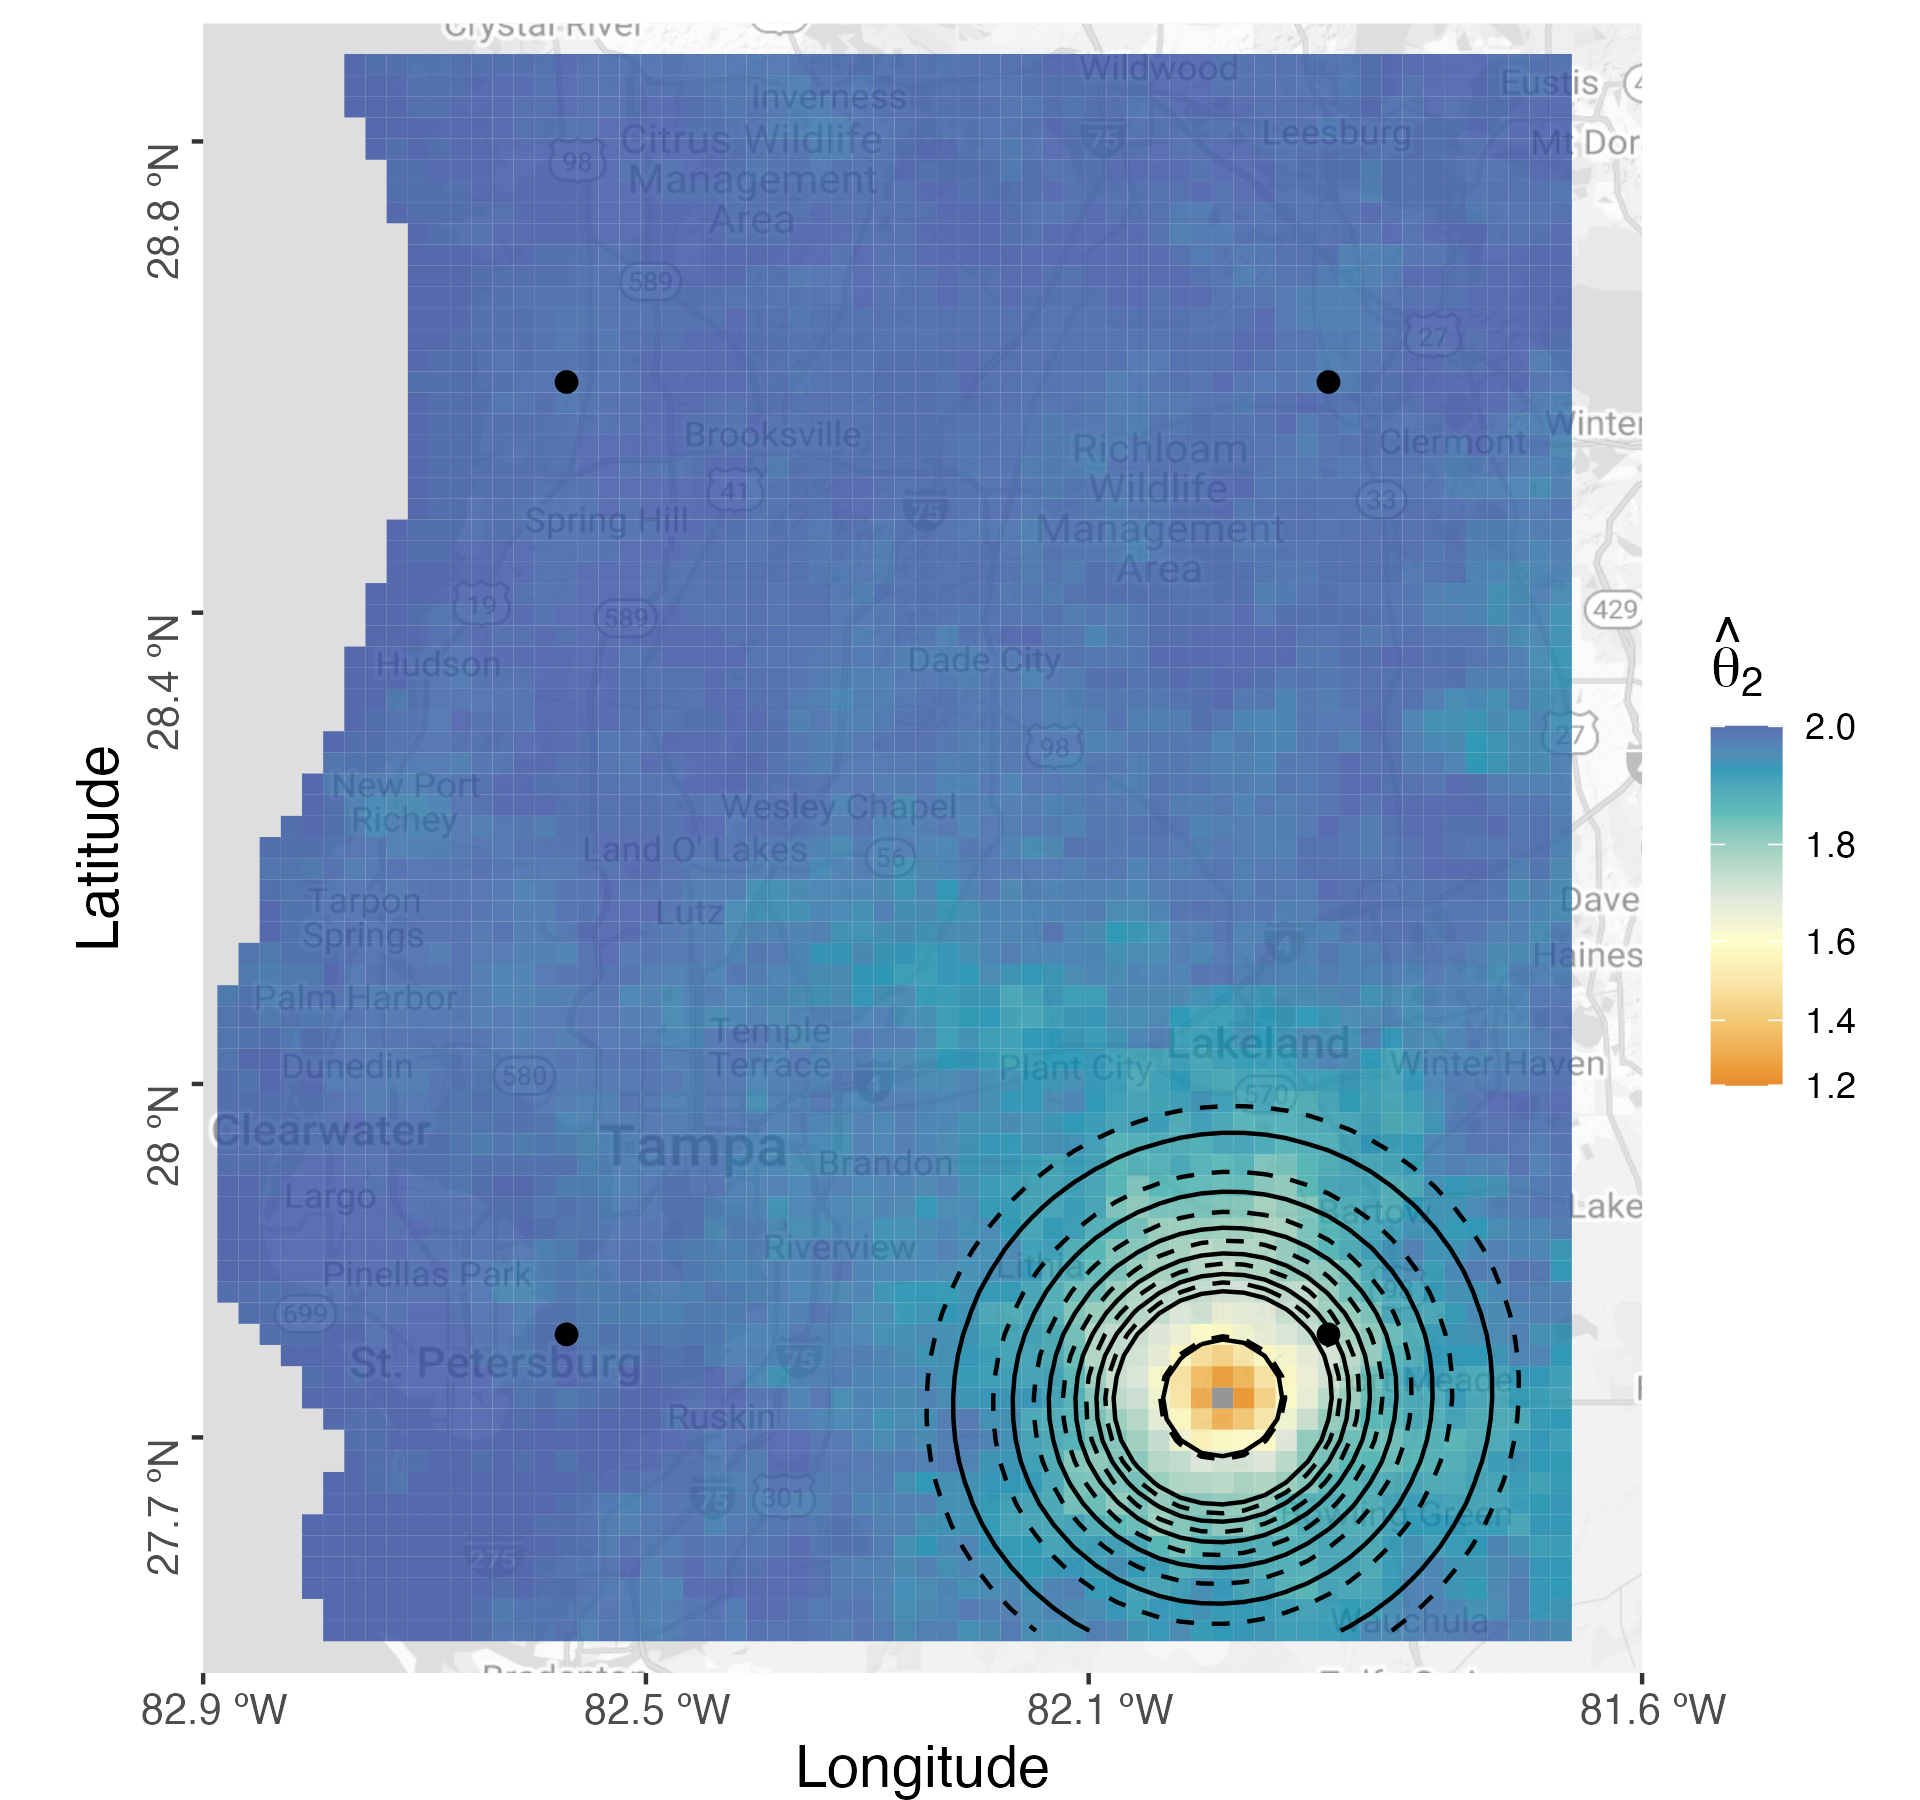
\includegraphics[width=1\textwidth]{florida/florida_extcoef_2_005.png}
    \end{subfigure}
    \begin{subfigure}{0.45\textwidth}
        \centering
        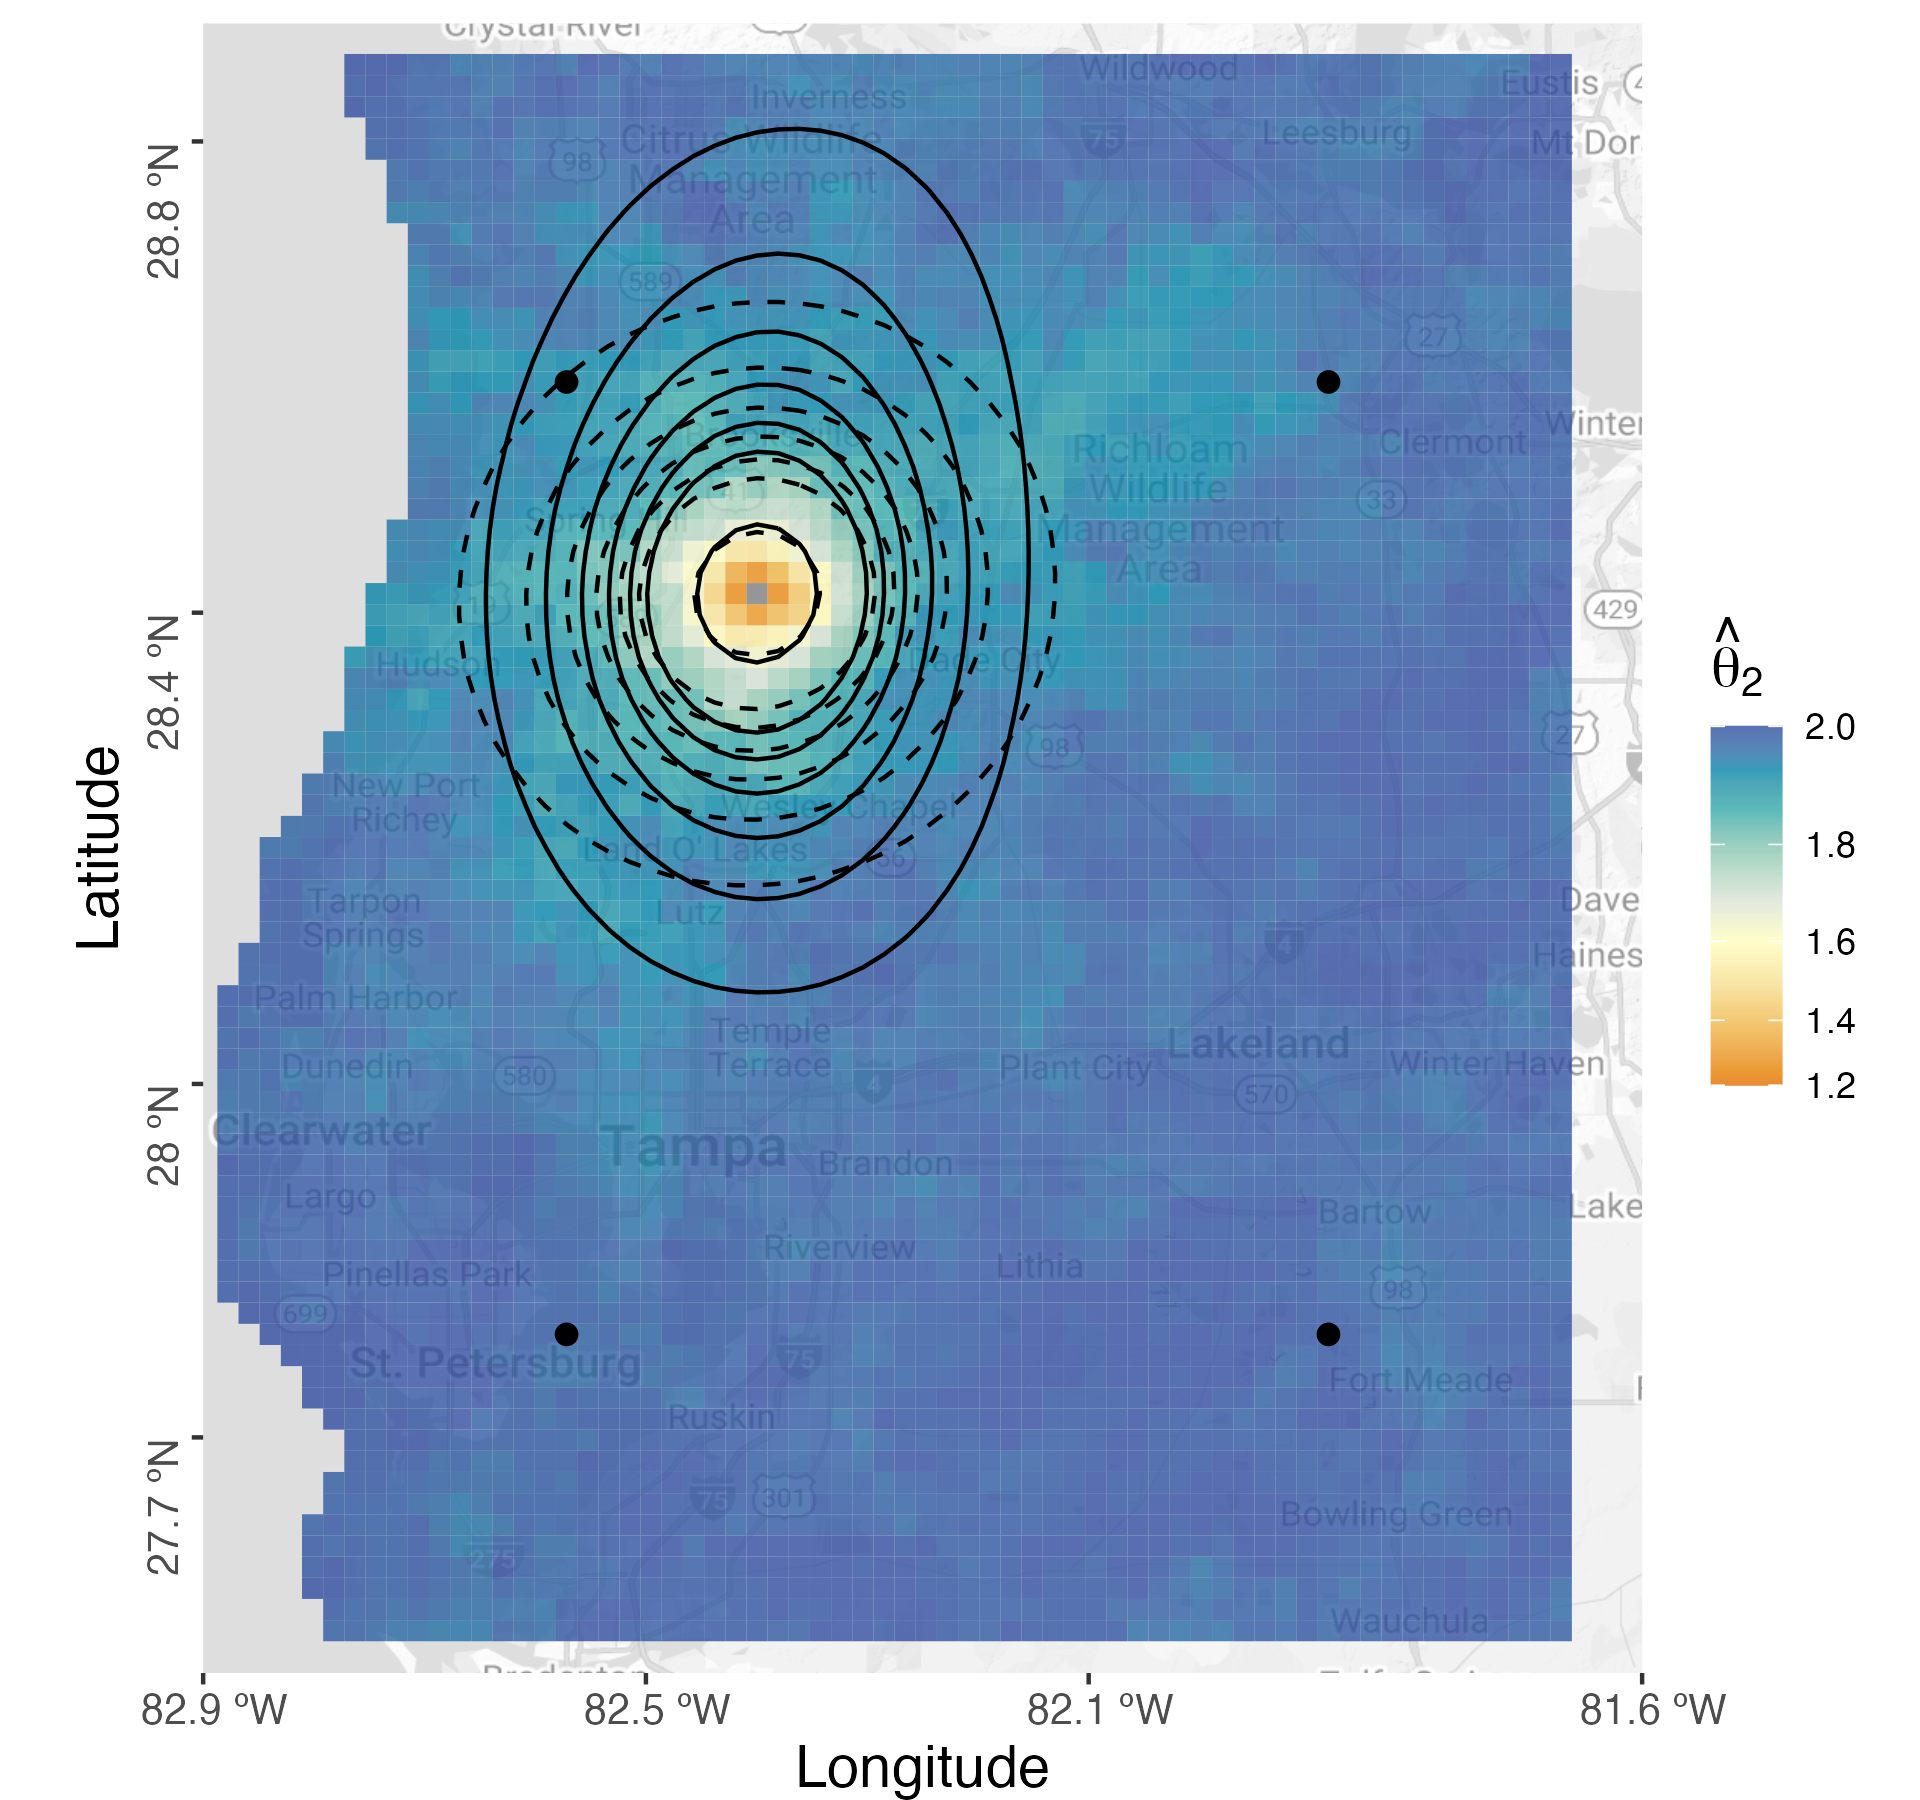
\includegraphics[width=1\textwidth]{florida/florida_extcoef_2_034.png}
    \end{subfigure}
    \caption{Maps of bivariate empirical extremal coefficients with respect to two different reference point, and the fitted extremal coefficient contour curves based on the fitted skewed Brown-Resnick r-Pareto process (solid) and Brown-Resnick r-Pareto process (dashed). The top row is for the $L_1$ norm risk functional and the bottom row is for the $L_\infty$ norm risk functional. Black dots are the kernel centres used in the skewed Brown-Resnick model.}
    \label{fig:extcoef_application_florida}
\end{figure}

We now examine the spatial dependence structure of the sea surface temperature (in $^\circ \textrm{C}$) over the Red Sea, as previously considered by \cite{Huser.Zhong:2023}. The data comprise 31 annual maxima observations recorded at $D=1043$ gridded locations from 1985 to 2015. We follow \cite{Huser.Zhong:2023} and standardise the margins to the unit Fr\'echet scale. The Brown-Resnick and its skewed alternative are fitted using the spectral likelihood with a threshold $T=10\times D$, where 10 approximately corresponds to the $90\%$ quantile of a unit Fr\'echet distribution, leaving 9 observations for model fitting.

A similar spline representation of $\bm\eta$ to the simulation study is chosen, where $J=5$, and the kernel centres $\bm s_j^\star, j=1, \ldots, J$ are selected in the middle of the Red Sea, along the north-south axis, shown as the black dots in Figure~\ref{fig:extcoef_application}. We implement no background noise, so that $\eta_i=0, i=1, \ldots, D$, as only $\bm\xi$ needs to be estimated (instead of $\bm\eta$) and so the identifiability of $b_i,i=1,\dots,J$ is not a concern. Parameter estimates below indicate that the parameters are identifiable, due to the large number of locations and kernel spline used.

For the Brown-Resnick model, the parameter estimation takes $196$ seconds on a single core, yielding $\left( \hat{\lambda}, \hat{\vartheta}\right) = \left(69.04, 1.19\right)$ with jackknife standard deviations $(4.85,0.04)$. In comparison, the method of \cite{Huser.Zhong:2023}, relying on the pairwise composite likelihood with less than 2000 pairs, takes $31$ seconds using 32 cores while fixing the smoothness parameter $\vartheta$. In that context, with fixed $\vartheta$ the spectral likelihood takes $57$ seconds using a single core and produces similar results. The skewed Brown-Resnick estimates are $\left( \hat{\lambda}, \hat{\vartheta}, \hat{b_1}, \hat{b_2},\hat{b_3},\hat{b_4},\hat{b_5}\right) = \left(53.12,1.37,-86.99,29.74,-69.96,4.79, 120.59\right)$, which were obtained in 39.5 minutes using 12 cores.
%with the three-stage optimisation method. 
The estimated $\hat\lambda$ is smaller but the estimated $\hat\vartheta$ is larger than the corresponding estimates for the Brown-Resnick model, which is to be expected as the estimated skewed Brown-Resnick model more properly accounts for the dependence strength and structure compared with the Brown-Resnick model. The corresponding estimated standard deviations based on the jackknife are $(2.83,0.05,14.08,1.82,1.66,3.37,1.92)$, suggesting that only one of the estimated slant parameters is insignificant.
% Finally, since the two models are nested, the Akaike Information Criterion can be used for model selection, confirming a better fit when including skewness in the distribution of the underlying process (AIC=-16458.04 versus -16430.1 for the Brown-Resnick).  

Maps of the bivariate extremal coefficient from the fitted Brown-Resnick and skewed Brown-Resnick models are given in Figure~\ref{fig:extcoef_application} for two reference locations. The right panels display empirical estimates which indicate the presence of some non-stationarity. The shape of the dependence structure estimated by the skewed Brown-Resnick model appears more realistic and better reflects the empirical observations. For example, there seems to be a region in the north of the Red Sea that is mildly dependent on the second reference point (bottom right panel) which is well captured by the skewed Brown-Resnick model (bottom left), and not at all by the Brown-Resnick model. 

\begin{figure}[!ht]
    \centering
    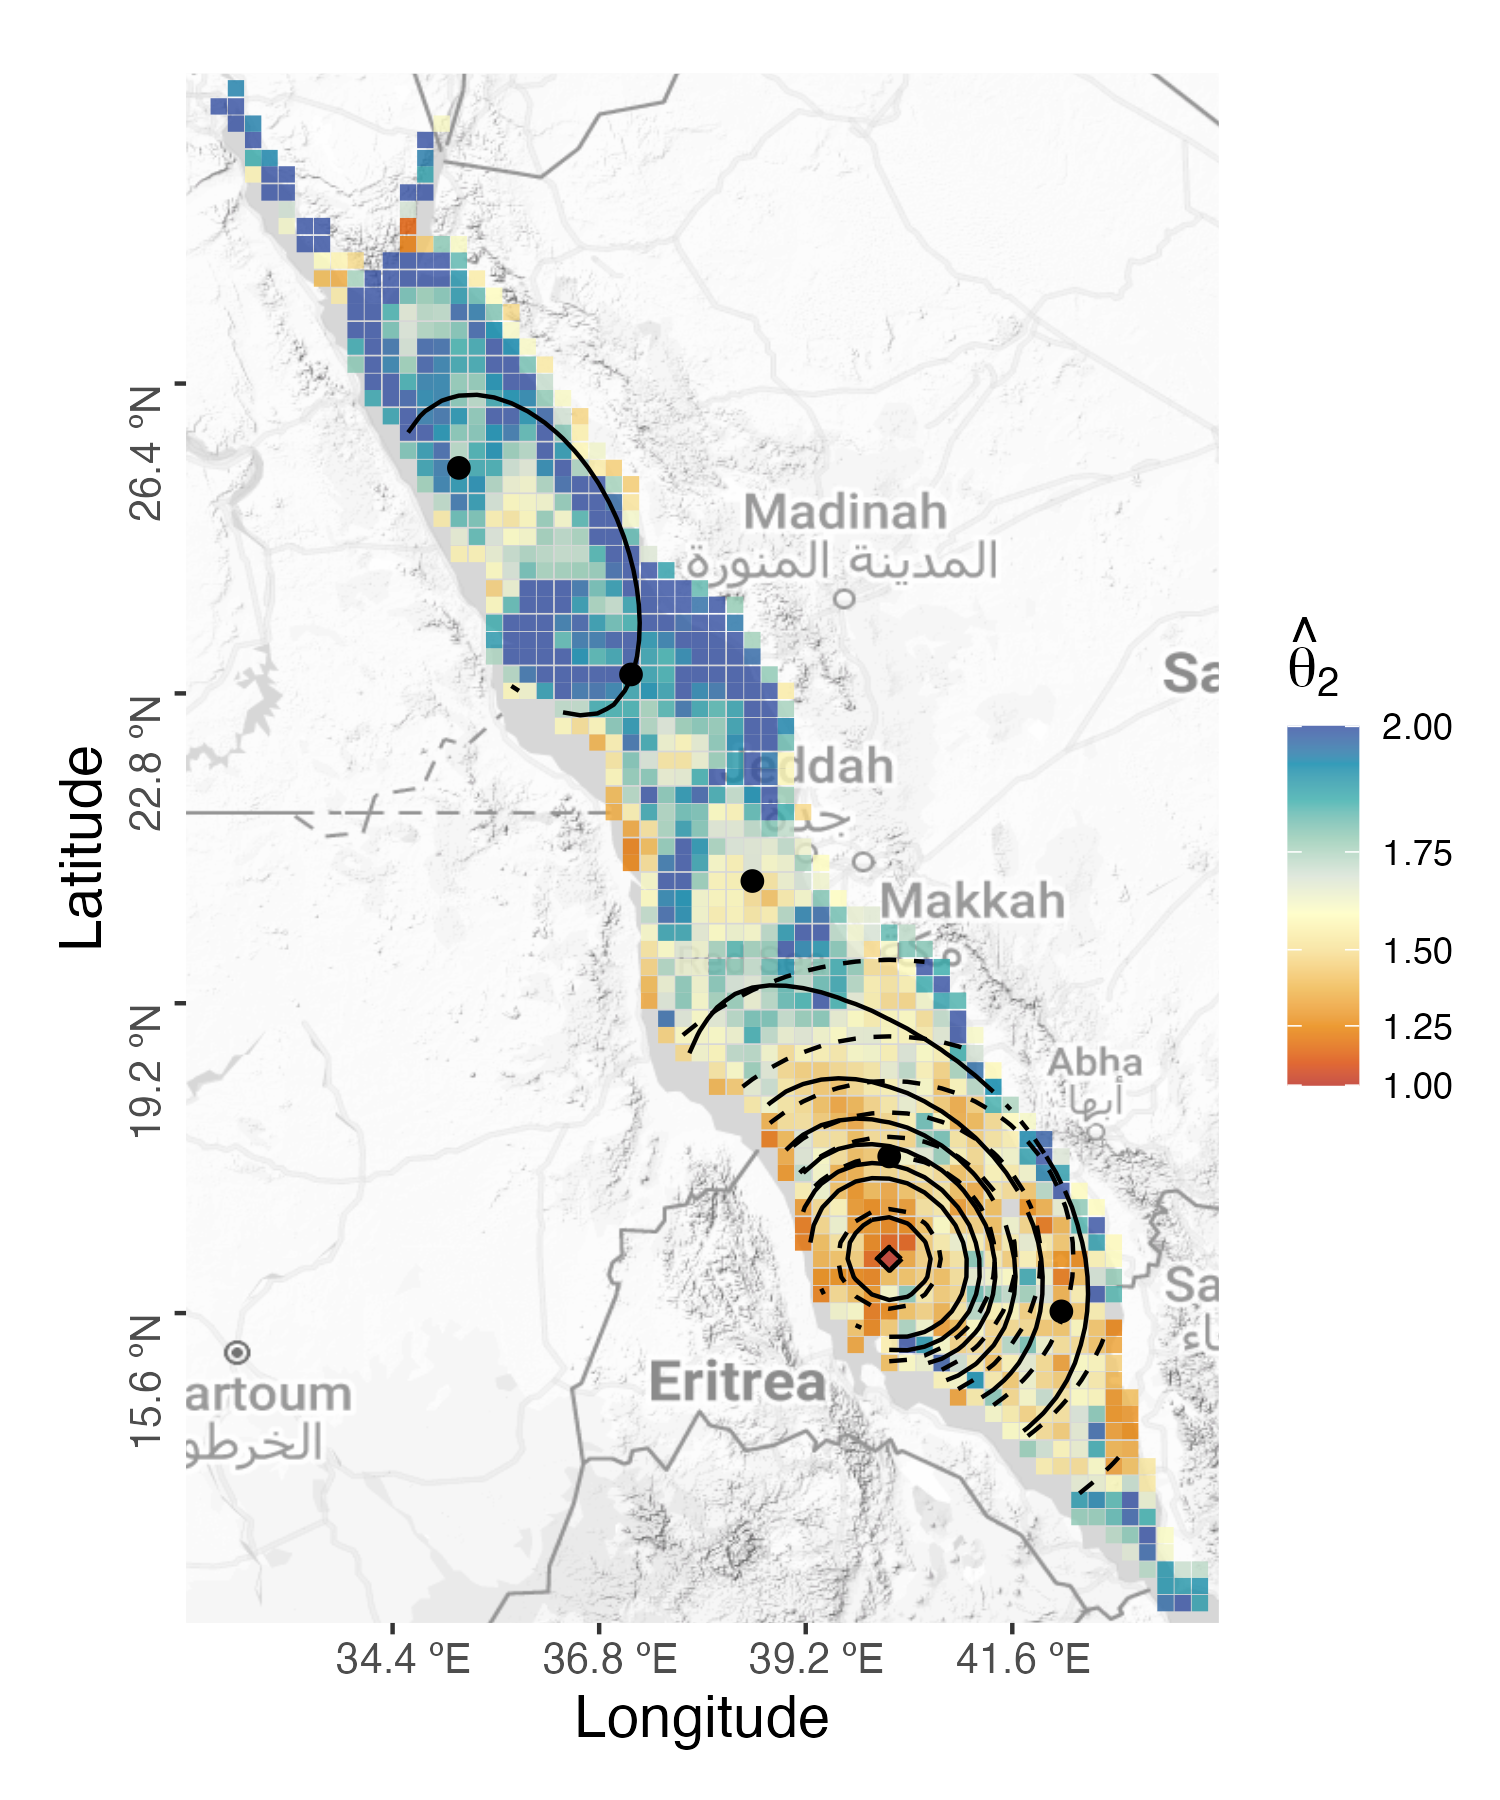
\includegraphics[width=0.49\textwidth]{RedSea2/RedSea_extcoef_MS_022.png}
    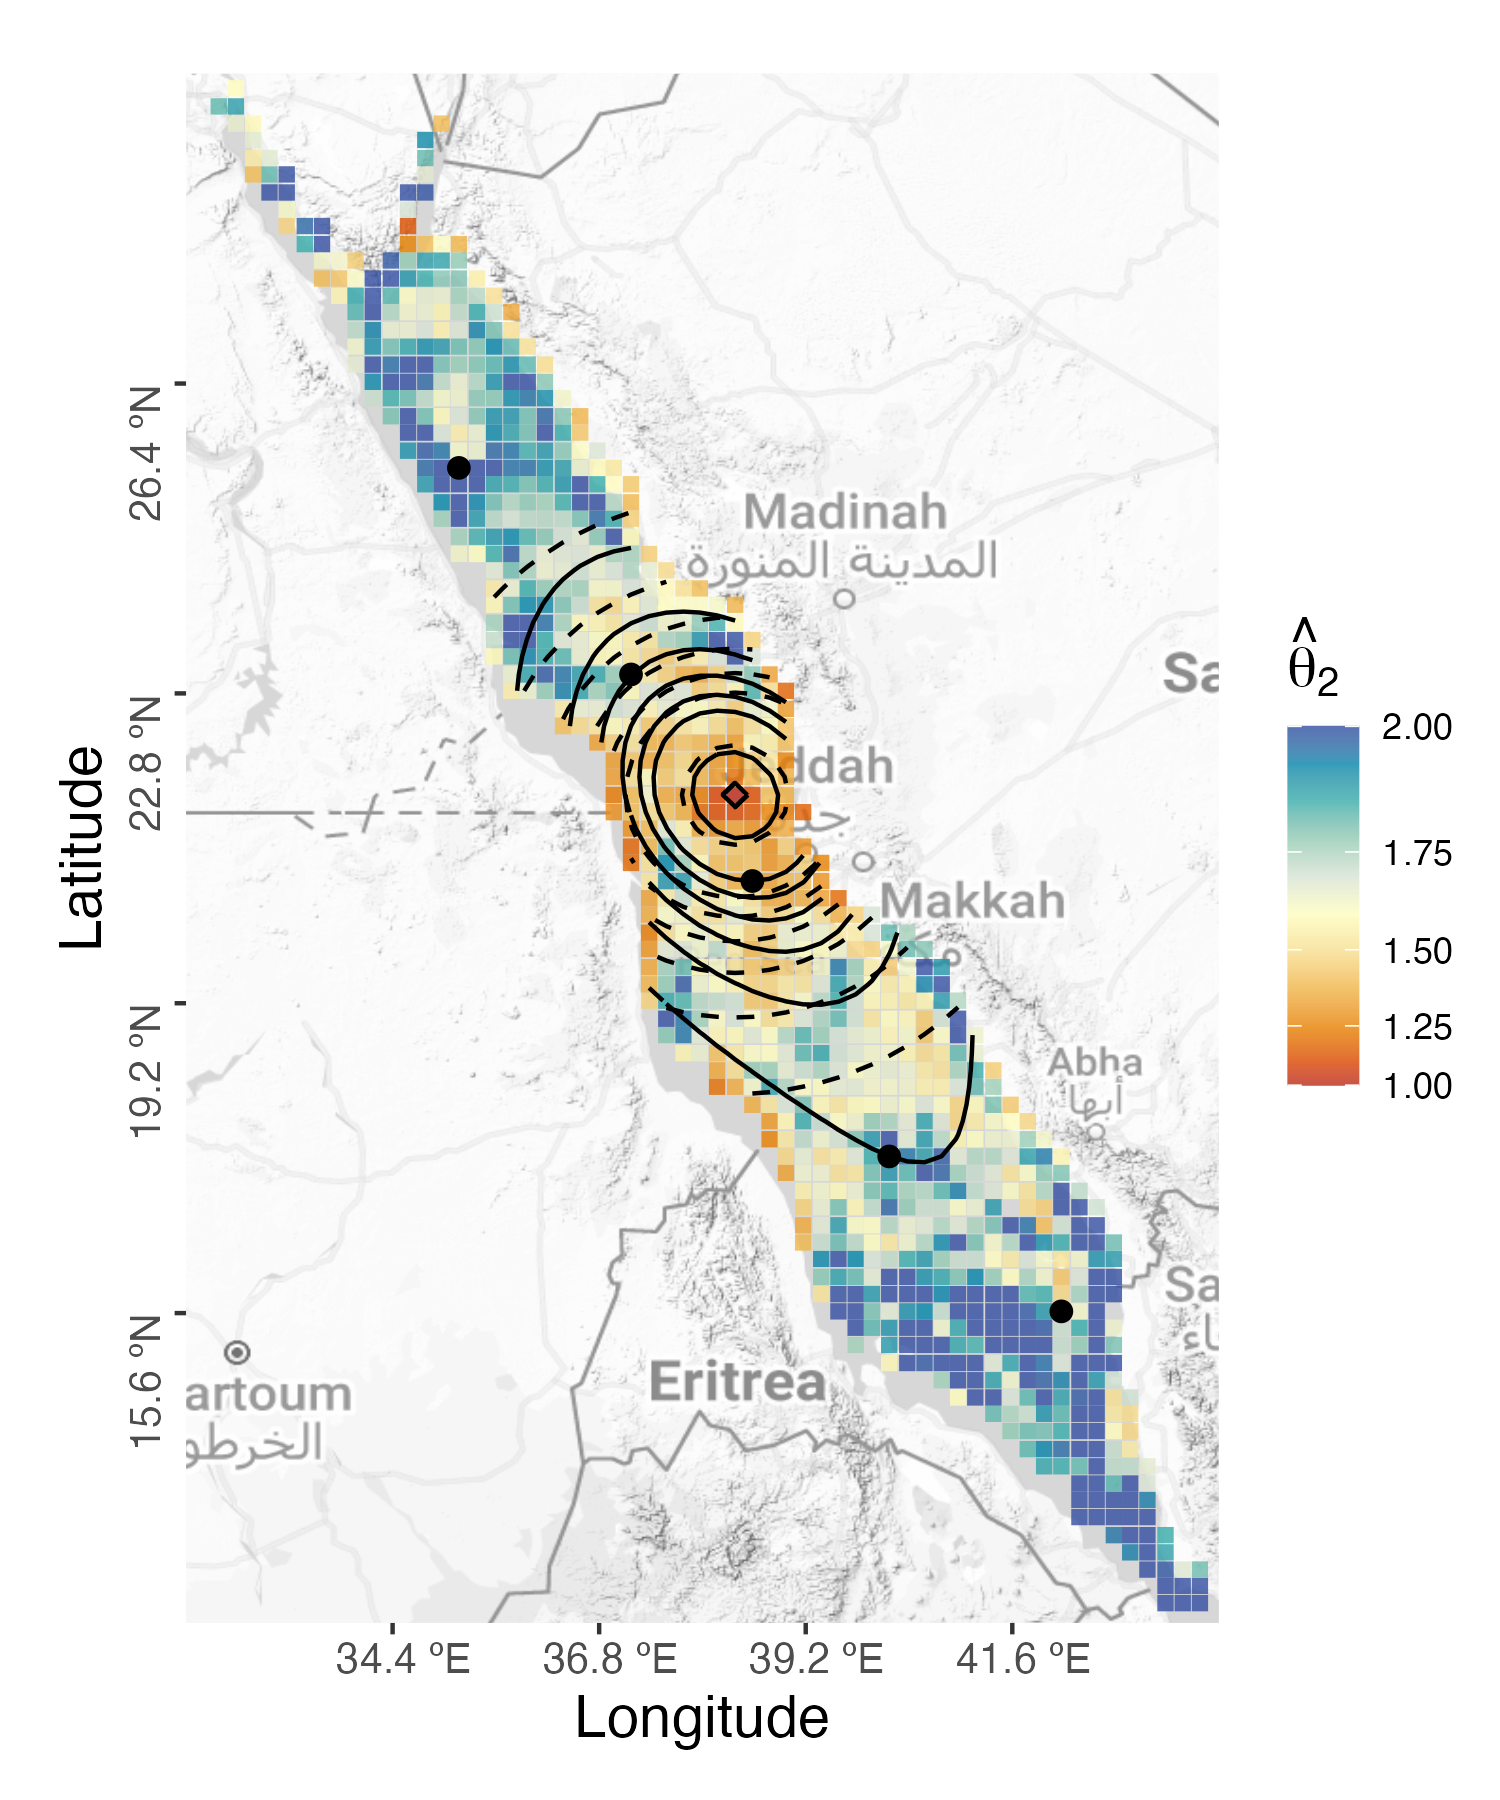
\includegraphics[width=0.49\textwidth]{RedSea2/RedSea_extcoef_MS_065.png}
    \caption{Maps of bivariate empirical extremal coefficient with respect to the centre labeled by the square symbol together with contours curves of the fitted extremal coefficients based on skewed Brown-Resnick (solid) and Brown-Resnick (dashed) models. Black dots are the kernel centres used in the skewed Brown-Resnick model.}
    \label{fig:extcoef_application}
\end{figure}

\section{Discussion}
We have proposed a class of models for spatial extreme modeling whose angular density does not have mass on the boundary space and avoids computing partial derivatives of the exponent function, the number of which quickly becomes intractable as the dimension of the data increases. 
%In particular, the methodology can easily be applied to very high dimensional data under the condition that the angular density only puts mass on the interior of the unit simplex $\Omega$ and, as such, 
We have established general conditions for a model to possess such property. The well-known Brown-Resnick process falls within this family of models and we derive two new extreme models: the \emph{skewed Brown-Resnick}, an extension of the Brown-Resnick that can model non-stationarity and local anisotropy, and the \emph{truncated extremal-t}, the equivalent of the extremal-t but without mass on the subspaces of the simplex.  

Our simulation experiments have verified that, given an appropriately chosen threshold for the radial component, the spectral likelihood can perform as well as the pairwise composite likelihood and in some instances better, especially for our new skewed Brown-Resnick model, since pairwsie likelihood cannot pick up the local anisotropic dependence structure. As for r-Pareto processes, the score matching method is highly numerical unstable to produce reasonable estimates compared to the spectral likelihood method. The statistical efficiency of the methodology is paired with its computational efficiency which allows it to fit flexible models to dimensions in thousands, as illustrated on a real dataset, within a reasonable timeframe. The advantages of the proposed methodology over the recent work of \citet{Huser.Zhong:2023} are also highlighted. Overall, this approach will help expand the usability of the asymptotic extreme models including max-stable and r-Pareto models in practice.  

The new models introduced in this manuscript are also a step towards building spatial extreme models suited for real-world problems and building extremal graphical models with flexible dependence structures as the only graphical extreme models are built based on Brown-Resnick model or H\"usler-Reiss model \citep{Engelke.Hitz:2020,Hentschel.Engelke.Segers:2024,Wan.Zhou:2023}. 

\section*{Supplemental Material}
The Supplemental Material contains the proofs of the theorems and propositions, and the exact simulation algorithms for the skewed Brown-Resnick and truncated extremal-t models. The code for the simulation study and the application is available at \url{https://github.com/PangChung/InteriorExtremes}. 

\section*{Acknowledgements}
This work was supported by the Australian Research Council (ARC) through the Discovery Project Scheme (DP220103269). 


%
\begin{table}[!ht]
    \centering
    \scalebox{0.85}{
        \begin{tabular}{cccccccccc|ccc}
            \hline
           Model & $\hat\lambda$ (km) & $\hat\vartheta$ & $\hat\zeta$ & $\hat m$ & $\hat b_1$ & $\hat b_2$ & $\hat b_3$ & $\hat b_4$ & $\hat b_5$ & AIC & time (s) \\ 
            \hline
            \multicolumn{13}{c}{Red Sea} \\ 
            \hline
            BR-SPEC & 64.78 & 1.16 & 0.79 & 1.14 & - & - & - & - & - & 1871.82 & 626.26 \\ 
            & (7.06) & (0.1) & (0.16) & (0.05) & & & & & & & &  \\
            sBR-SPEC & 51.36 & 1.33 & 0.79 & 1.12 & -13.49 & -8.31 & 2.05 & 12.85 & 15.07 & 1843.46 & 2336.44 \\ 
            & (4.75) & (0.09) & (0.28) & (0.07) &  (15.48) &  (6.76) &  (9.32) &   (7.58) & (11.47) & & \\
            BR-COMP & 58.61 & 1.35 & -0.54 & 0.76 & - & - & - & - & - & - & 3342.12 \\ 
            & (14.79) & (0.18) & (0.05) & (0.04) & & & & & & &  \\
            BR-VECC & 108.91 & 1.16 & 0.79 & 1.21 & - & - & - & - & - & - & 5062.01 \\ 
            & (12.2) & (0.09) & (0.10) & (0.06) &&&&&&& & \\
            \hline
            \multicolumn{13}{c}{Florida Tampa Bay} \\
            \hline
            BR-SUM-SPEC & 5.91 & 1.16 & -0.73 & 0.96 & 0.00 & 0.00 & 0.00 & 0.00 & - & 2485.88 & 4097.50 \\ 
            & (1.71) & (0.11) & (1.21) & (0.07) & & & & & & & &  \\
            BR-MAX-SPEC & 6.30 & 1.37 & 0.40 & 0.95 & 0.00 & 0.00 & 0.00 & 0.00 & - & 2526.61 & 6126.39 \\ 
            & (0.39) & (0.03) & (0.36) & (0.04)  & & & & & & & & \\
            sBR-SUM-SPEC & 5.81 & 1.19 & 0.73 & 1.04 & 11.39 & 8.58 & 23.09 & 19.89 & - & 2482.39 & 15111.80 \\  
            & (1.74) & (0.11) & (2.83) & (0.15) & (27.15) & (21.37) & (56.21) & (47.90) & & & \\
            sBR-MAX-SPEC & 5.96 & 1.41 & 0.46 & 0.96 & 0.16 & 0.15 & 0.06 & 0.07 & - & 2510.44 & 17777.21  \\
            & (0.35) & (0.03) & (0.28) & (0.04) & (1.22) & (1.22) & (0.52) & (0.48) & & & \\
            BR-SUM-SCORE & 2.80 & 1.40 & -0.12 & 1.06 & 0.00 & 0.00 & 0.00 & 0.00 & - & - & 7396.65 \\ 
            & (0.25) & (0.09) & (1.25) & (0.07) &&&&&&&&  \\
            BR-MAX-SCORE & 3.49 & 1.71 & -0.04 & 1.02 & 0.00 & 0.00 & 0.00 & 0.00 & - & - & 6852.99 \\ 
            & (0.22) & (0.04) & (1.83) & (0.05) &&&&&&&&  \\
        \end{tabular}
    }
    \caption{}
    \label{tab:parameter_estimates}
\end{table}


\baselineskip=18pt
\bibliographystyle{CUP}
\bibliography{Total.bib}
\end{document}
